% $Id: appendix.tex 93220 2016-06-08 09:56:19Z michaelt $
% ===============================================================================
% Purpose: appendix to the standard template: standard symbol alises from Ulrik
% Author: Tomasz Skwarnicki
% Created on: 2009-09-24
% ===============================================================================

\clearpage
\begin{savequote}[8cm]
\textlatin{Cor animalium, fundamentum e\longs t vitæ, princeps omnium, Microco\longs mi Sol, a quo omnis vegetatio dependet, vigor omnis \& robur emanat.}

The heart of animals is the foundation of their life, the sovereign of everything within them, the sun of their microcosm, that upon which all growth depends, from which all power proceeds.
  \qauthor{--- William Harvey \cite{harvey_exercitatio_1628}}
\end{savequote}

\chapter{\label{app:1-cardiophys}Review of Cardiac Physiology and Electrophysiology}

\minitoc
%\appendix
\section{Stripping requirements}
\label{sec:app:stripping}

$B^{\pm} \to DK^{*\pm}$ candidates were selected using stripping lines in the {\tt BHADRON} stripping stream, {\tt B2D0KsPiLLD2HHBeauty2CharmLine} and {\tt B2D0KsPiDDD2HHBeauty2CharmLine}. The stripping requirements are summarized in Table \ref{strippingrequirements}. These stripping lines also have the requirement that one of the following Hlt2 trigger lines must be fired: Hlt2Topo.*DecisionTIS, Hlt2Topo.*DecisionTOS, Hlt2IncPhi.*DecisionTIS or Hlt2IncPhi.*DecisionTOS.

\begin{table}[h]
\centering
\begin{tabular}{lll}
\hline
Particle & Variable & Cut value \\
\hline
Charged track & $p_T$ & $>$ 100 \mevc \\
& $p$ & $>$ 1000 \mevc \\
& Min IP $\chi^2$ & $>$ 4 \\
\hline
\KS & $p_T$ & $>$ 250 \mevc \\
& Vertex $\chi^2$/ndof & $<$ 25 \\
& \textbar M(\KS) - 497.6 \mevcc \textbar & $<$ 35 \mevcc for LL, 64 \mevcc for DD \\
& Measured mass (MM) & $\in$ [467,527] \mevcc \\
\hline
\KS daughters & $p$ & $>$ 2 \gevc \\
& Min IP $\chi2$ PV & $>$ 9 for LL, 4 for DD \\ 
\hline
Bachelor pion & Track $\chi^2$/ndof & $<$ 2.5 ($<$ 4 in S26) \\
& $p_T$ & $>$ 250 \mevc \\
& $p$ & $>$ 2500 \mevc \\
\hline
\Bpm & Vertex $\chi^2$/ndof & $<$ 10 \\
& Min IP $\chi^2$ & $<$ 25 \\
& $\tau$ & $>$ 0.2 ps \\
& cos($\theta_{dira}$) & $>$ 0.999 \\
& M(\Dz\KS\pion) & $\in$ [4750,5800] \mevcc \\
\hline
\end{tabular}
\caption{Summary of the stripping selection requirements for \decay{\Bpm}{\D\Kstarpm} candidates}
\label{strippingrequirements}
\end{table}

\clearpage

\section{Charmless background}
\label{sec:app:charmless}

Figures \ref{allchamrmless0Run1} and \ref{allchamrmless5Run1} show the fits to data in the D mass sidebands after a \Dz FD significance cut of zero and 5 respectively for Run 1 data. Figures \ref{allchamrmless0Run2} and \ref{allchamrmless5Run2} show the equivalent plots for Run 2 data. Plots show that the charmless contribution is reduced to a negligible level in all modes except for \decay{\Dz}{\pip\pim} where there may still be a residual contribution. 

\begin{figure}[h]
\centering
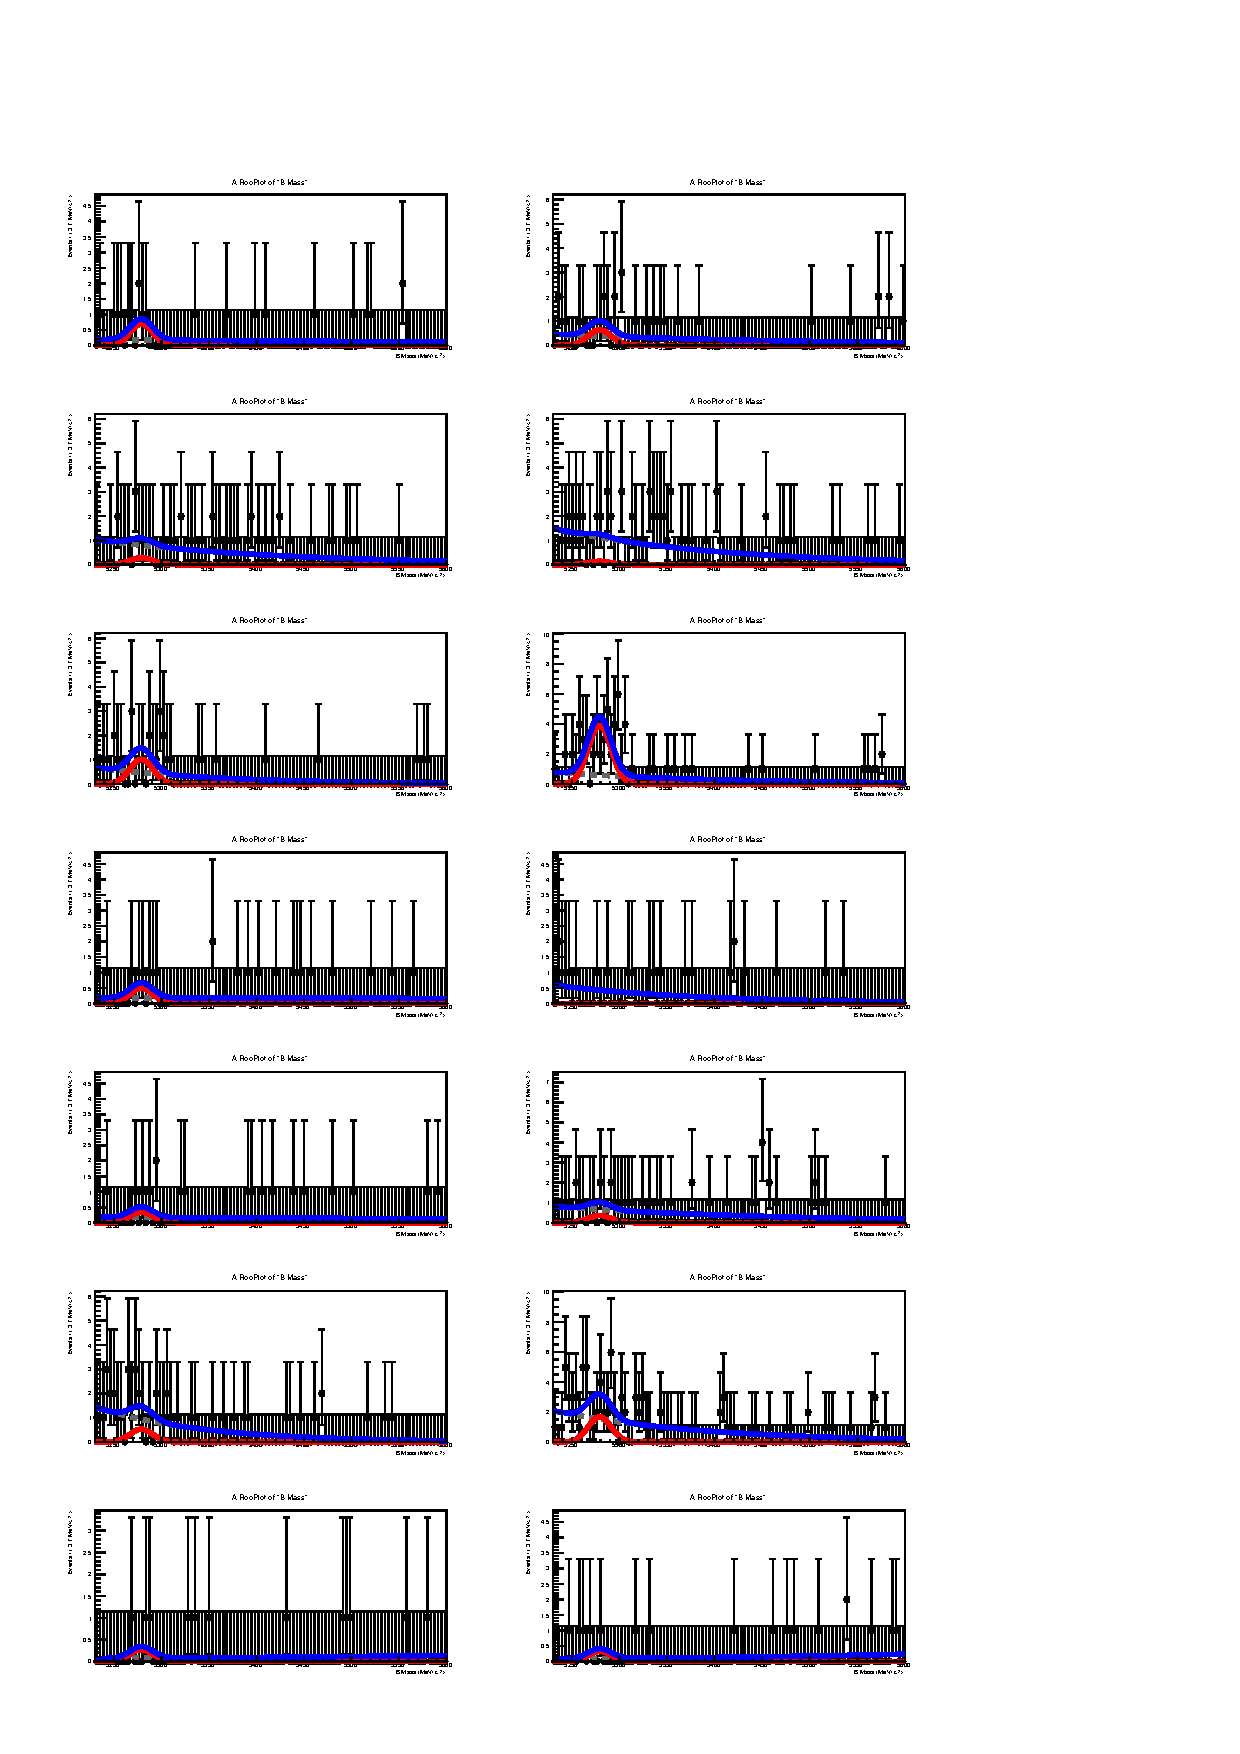
\includegraphics[width=0.65\linewidth]{figures/backgrounds/charmlessFits_FD0_run1.pdf}
\put(-250,470) {(a)}
\put(-100,470) {(b)}
\put(-250,400) {(c)}
\put(-100,400) {(d)}
\put(-250,330) {(e)}
\put(-100,330) {(f)}
\put(-250,260) {(g)}
\put(-100,260) {(h)}
\put(-250,190) {(i)}
\put(-100,190) {(j)}
\put(-250,120) {(k)}
\put(-100,120) {(l)}
\put(-250,40) {(m)}
\put(-100,40) {(n)}
\caption{Fits to be refitted B mass taking candidates from the D mass sidebands after a FD significance cut of zero for (a) $K\pi$ LL, (b) $K\pi$ DD, (c) $KK$ LL, (d) $KK$ DD, (e) $\pi\pi$ LL, (f) $\pi\pi$ DD, (g) $\pi K$ LL, (h) $\pi K$ DD, (i) $K\pi\pi\pi$ LL, (j) $K\pi\pi\pi$ DD, (k) $\pi\pi\pi\pi$ LL, (l) $\pi\pi\pi\pi$ DD, (m) $\pi K\pi\pi$ LL, and (n) $\pi K\pi\pi$ DD.. A Gaussian is used to model the signal and an exponential for the combinatoric background}
\label{allchamrmless0Run1}
\end{figure}

\begin{figure}[h]
\centering
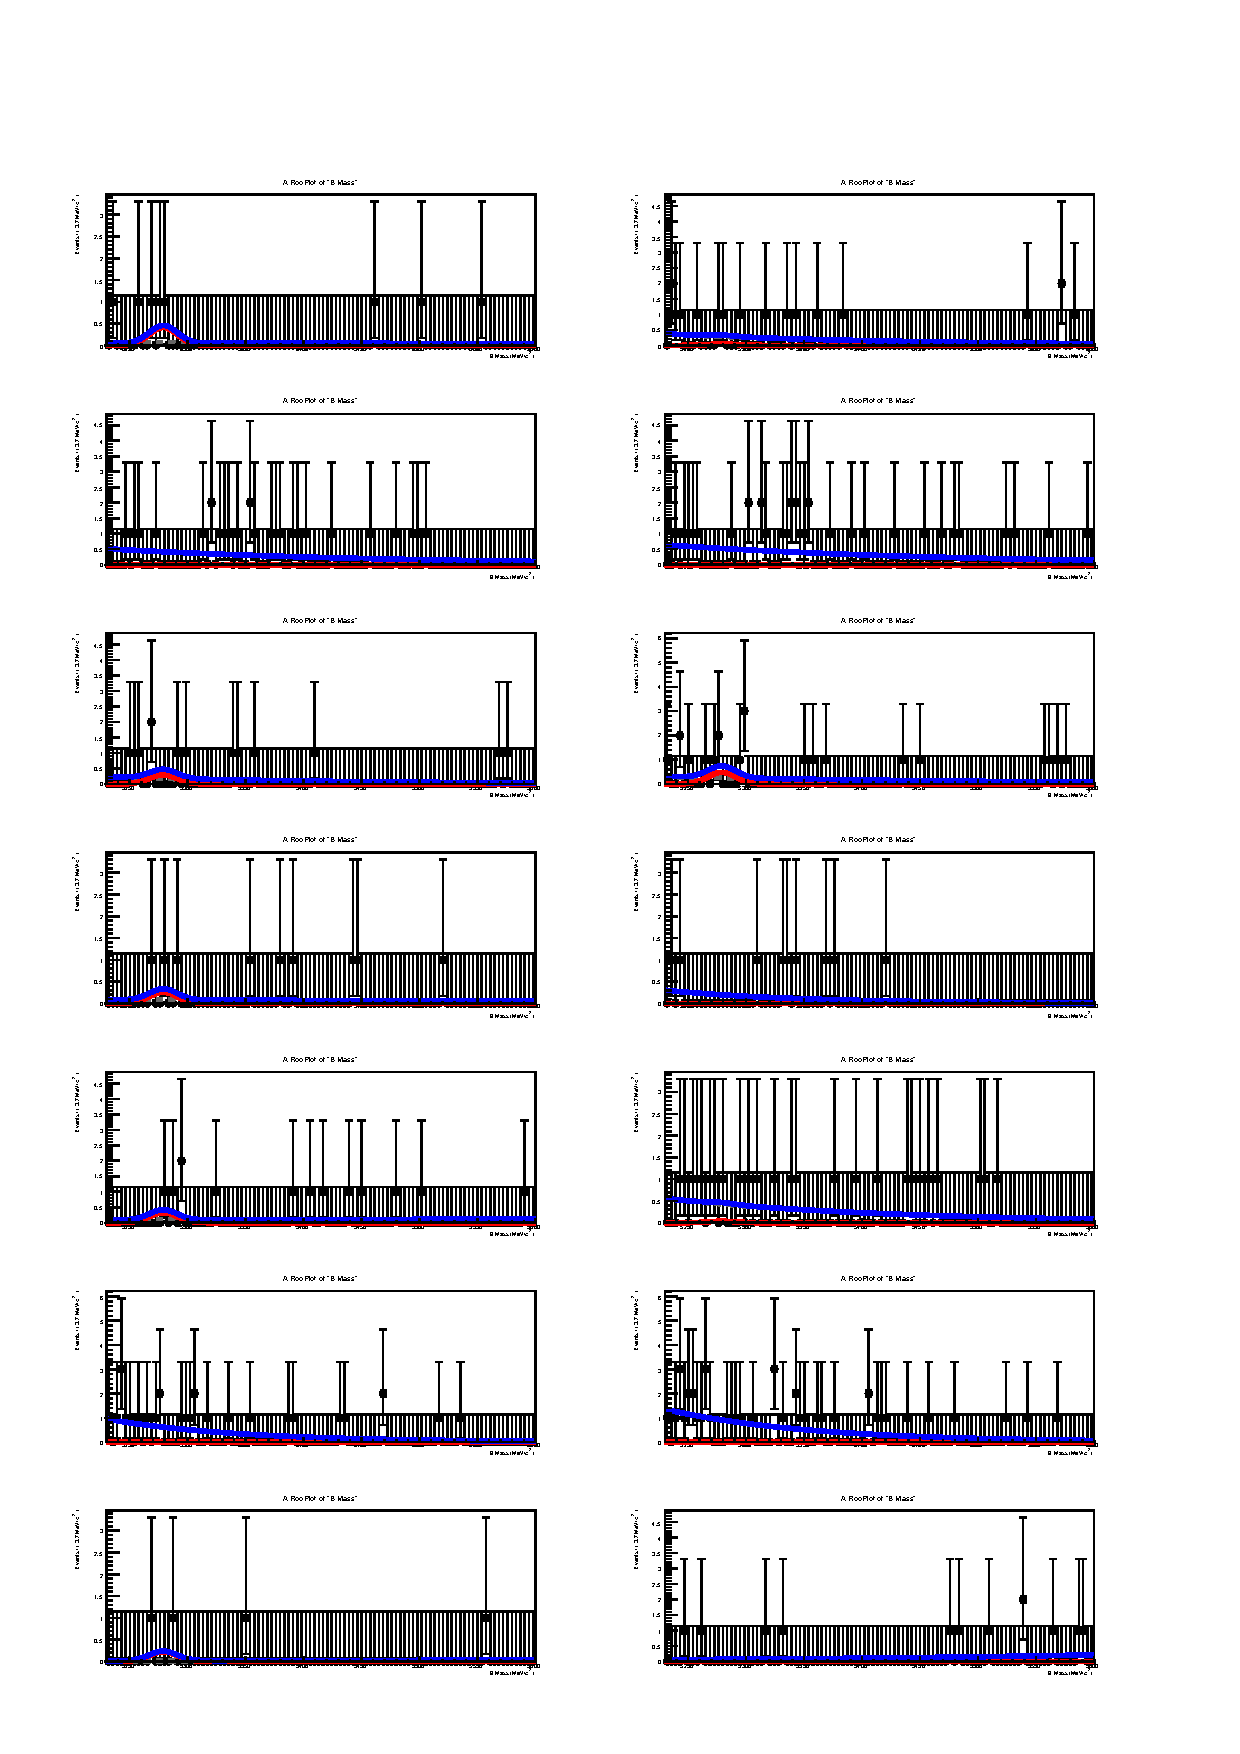
\includegraphics[width=0.8\linewidth]{figures/backgrounds/charmlessFits_FD2_run1.pdf}
\put(-250,470) {(a)}
\put(-100,470) {(b)}
\put(-250,400) {(c)}
\put(-100,400) {(d)}
\put(-250,330) {(e)}
\put(-100,330) {(f)}
\put(-250,260) {(g)}
\put(-100,260) {(h)}
\put(-250,190) {(i)}
\put(-100,190) {(j)}
\put(-250,120) {(k)}
\put(-100,120) {(l)}
\put(-250,40) {(m)}
\put(-100,40) {(n)}
\caption{Fits to be refitted B mass taking candidates from the D mass sidebands after a FD significance cut of 2$\sigma$ for (a) $K\pi$ LL, (b) $K\pi$ DD, (c) $KK$ LL, (d) $KK$ DD, (e) $\pi\pi$ LL, (f) $\pi\pi$ DD, (g) $\pi K$ LL, (h) $\pi K$ DD, (i) $K\pi\pi\pi$ LL, (j) $K\pi\pi\pi$ DD, (k) $\pi\pi\pi\pi$ LL, (l) $\pi\pi\pi\pi$ DD, (m) $\pi K\pi\pi$ LL, and (n) $\pi K\pi\pi$ DD.. A Gaussian is used to model the signal and an exponential for the combinatoric background}
\label{allchamrmless5Run1}
\end{figure}

\begin{figure}[h]
\centering
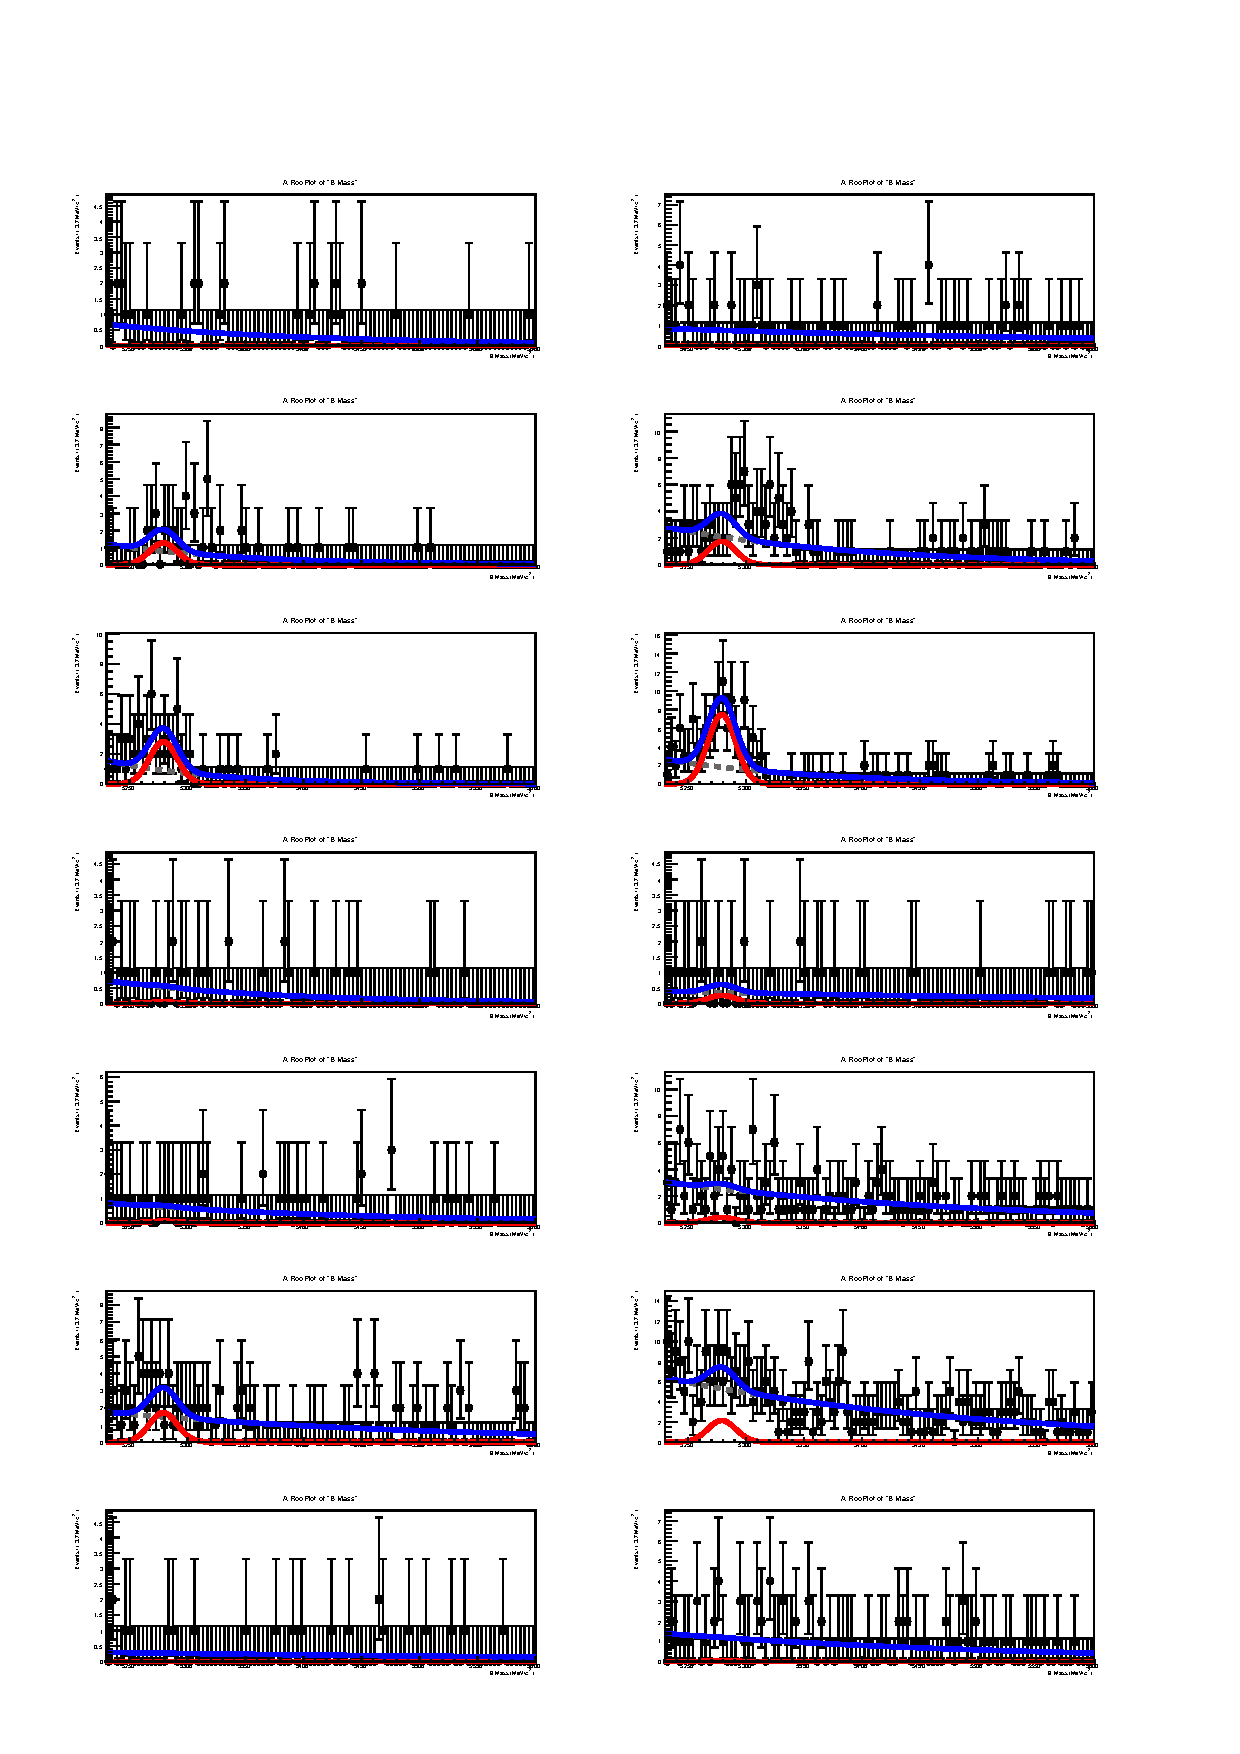
\includegraphics[width=0.8\linewidth]{figures/backgrounds/charmlessFits_FD0_run2.pdf}
\put(-250,470) {(a)}
\put(-100,470) {(b)}
\put(-250,400) {(c)}
\put(-100,400) {(d)}
\put(-250,330) {(e)}
\put(-100,330) {(f)}
\put(-250,260) {(g)}
\put(-100,260) {(h)}
\put(-250,190) {(i)}
\put(-100,190) {(j)}
\put(-250,120) {(k)}
\put(-100,120) {(l)}
\put(-250,40) {(m)}
\put(-100,40) {(n)}
\caption{Fits to be refitted B mass taking candidates from the D mass sidebands after a FD significance cut of zero for (a) $K\pi$ LL, (b) $K\pi$ DD, (c) $KK$ LL, (d) $KK$ DD, (e) $\pi\pi$ LL, (f) $\pi\pi$ DD, (g) $\pi K$ LL, (h) $\pi K$ DD, (i) $K\pi\pi\pi$ LL, (j) $K\pi\pi\pi$ DD, (k) $\pi\pi\pi\pi$ LL, (l) $\pi\pi\pi\pi$ DD, (m) $\pi K\pi\pi$ LL, and (n) $\pi K\pi\pi$ DD.. A Gaussian is used to model the signal and an exponential for the combinatoric background}
\label{allchamrmless0Run2}
\end{figure}

\begin{figure}[h]
\centering
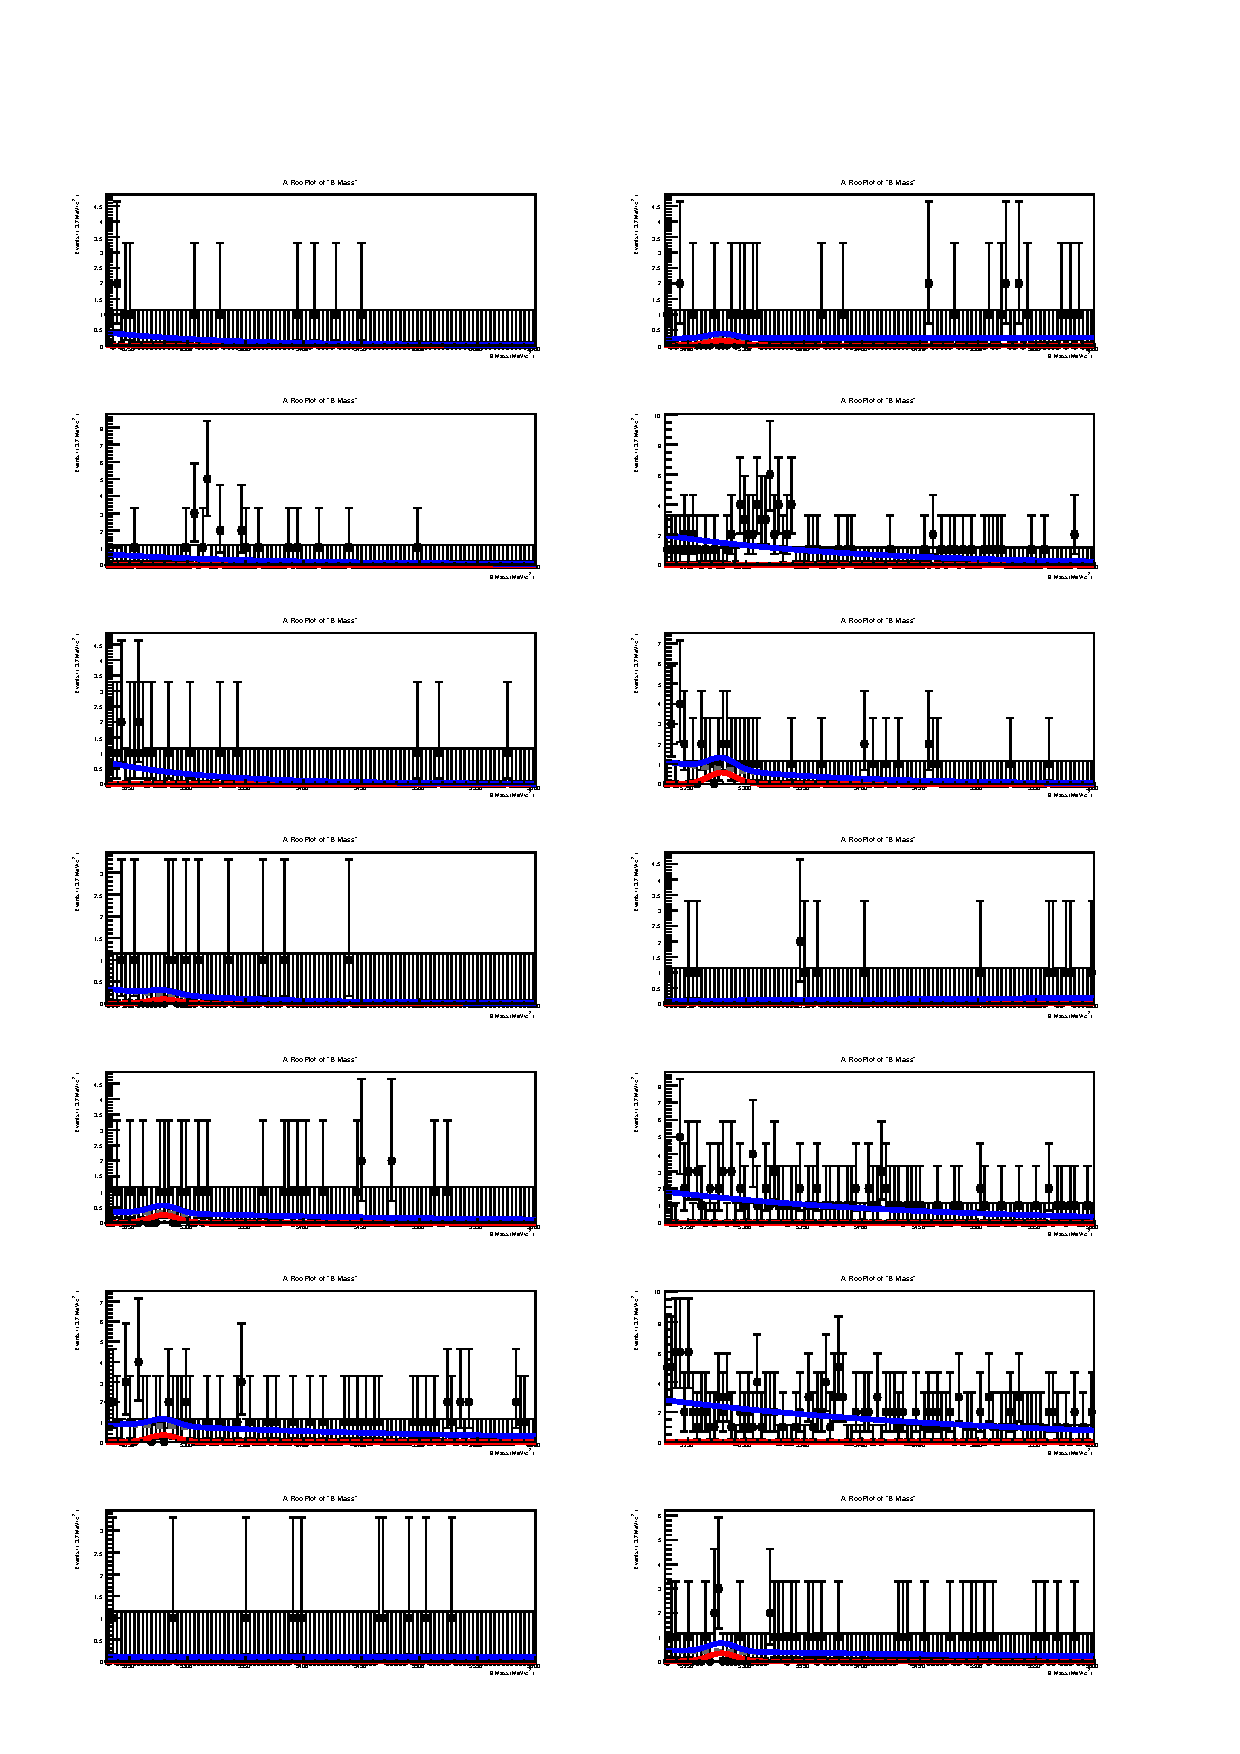
\includegraphics[width=0.8\linewidth]{figures/backgrounds/charmlessFits_FD2_run2.pdf}
\put(-250,470) {(a)}
\put(-100,470) {(b)}
\put(-250,400) {(c)}
\put(-100,400) {(d)}
\put(-250,330) {(e)}
\put(-100,330) {(f)}
\put(-250,260) {(g)}
\put(-100,260) {(h)}
\put(-250,190) {(i)}
\put(-100,190) {(j)}
\put(-250,120) {(k)}
\put(-100,120) {(l)}
\put(-250,40) {(m)}
\put(-100,40) {(n)}
\caption{Fits to be refitted B mass taking candidates from the D mass sidebands after a FD significance cut of 2$\sigma$ for (a) $K\pi$ LL, (b) $K\pi$ DD, (c) $KK$ LL, (d) $KK$ DD, (e) $\pi\pi$ LL, (f) $\pi\pi$ DD, (g) $\pi K$ LL, (h) $\pi K$ DD, (i) $K\pi\pi\pi$ LL, (j) $K\pi\pi\pi$ DD, (k) $\pi\pi\pi\pi$ LL, (l) $\pi\pi\pi\pi$ DD, (m) $\pi K\pi\pi$ LL, and (n) $\pi K\pi\pi$ DD. A Gaussian is used to model the signal and an exponential for the combinatoric background}
\label{allchamrmless5Run2}
\end{figure}

\clearpage

\section{\KS helicity angle}
\label{sec:app:helicityangle}

Figure \ref{helicitycut} shows that the MC distribution of the cosine of Ks helicity angle is asymmetric. Physically the Ks helicity angle is expected to follow a symmetric $cos^2\theta$ distribution, however the observed asymmetry in this variable, manifest in both data and MC, was found to be due to the momentum and transverse momentum cuts placed on the bachelor pion in the stripping line. Figure \ref{helictyasymmetry} illustrates this point.

\begin{figure}[h]
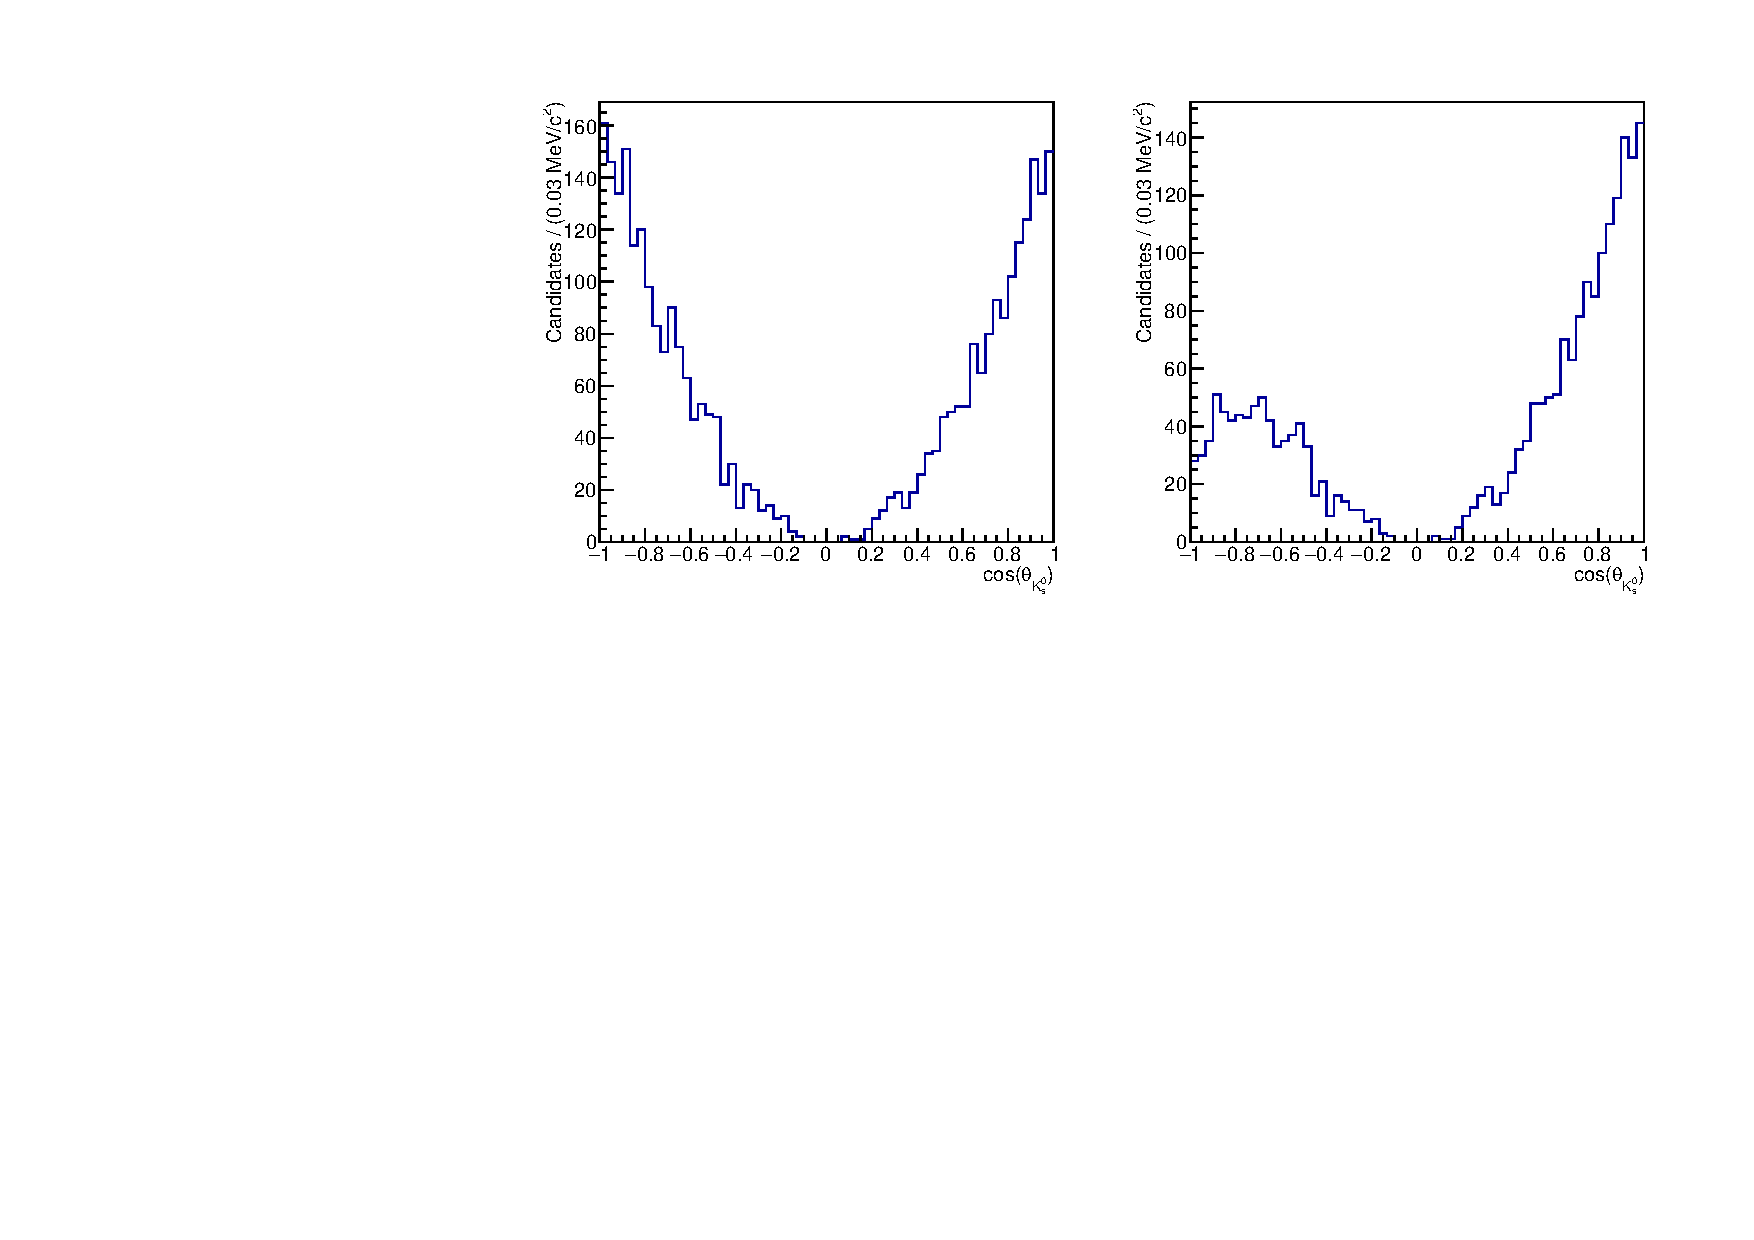
\includegraphics[width=\linewidth]{figures/helicityAngleAsymmetry.pdf}
\put(-360,150) {(a)}
\put(-150,150) {(b)}
\caption{\KS helicity angle MC distribution at generator level with (a) no cuts applied, and (b) bachelor $p > 2500$ MeV and bachelor $p_T > 250$ MeV, as in the stripping line}
\label{helictyasymmetry}
\end{figure}

\clearpage

\section{Ignored backgrounds}
\label{sec:app:ignoredbackgrounds}


\subsubsection{\decay{\B}{\D\Kstar\piz}}

There is no measured branching fraction for \decay{\B}{\D\Kstar\piz}. A \decay{\B}{\D\Kstar\piz} branching fraction of $6 \times 10^{-4}$ is assumed. The full selection is applied to 1M \decay{\B}{\D\Kstar\piz} events, Figure \ref{B2DKstPi0} shows the distribution of the remaining events. The estimated contribution in the favoured \decay{\B}{\D(\kaon\pi)\Kstar} mass fit is 3.6\% and 4.8\% of the signal, for LL and DD respectively, across the mass range 4750-5150 MeV. As the simultaneous fit has a mass range starting from 5230 MeV, this background is not considered for the mass fit.

\begin{figure}[h]
\centering
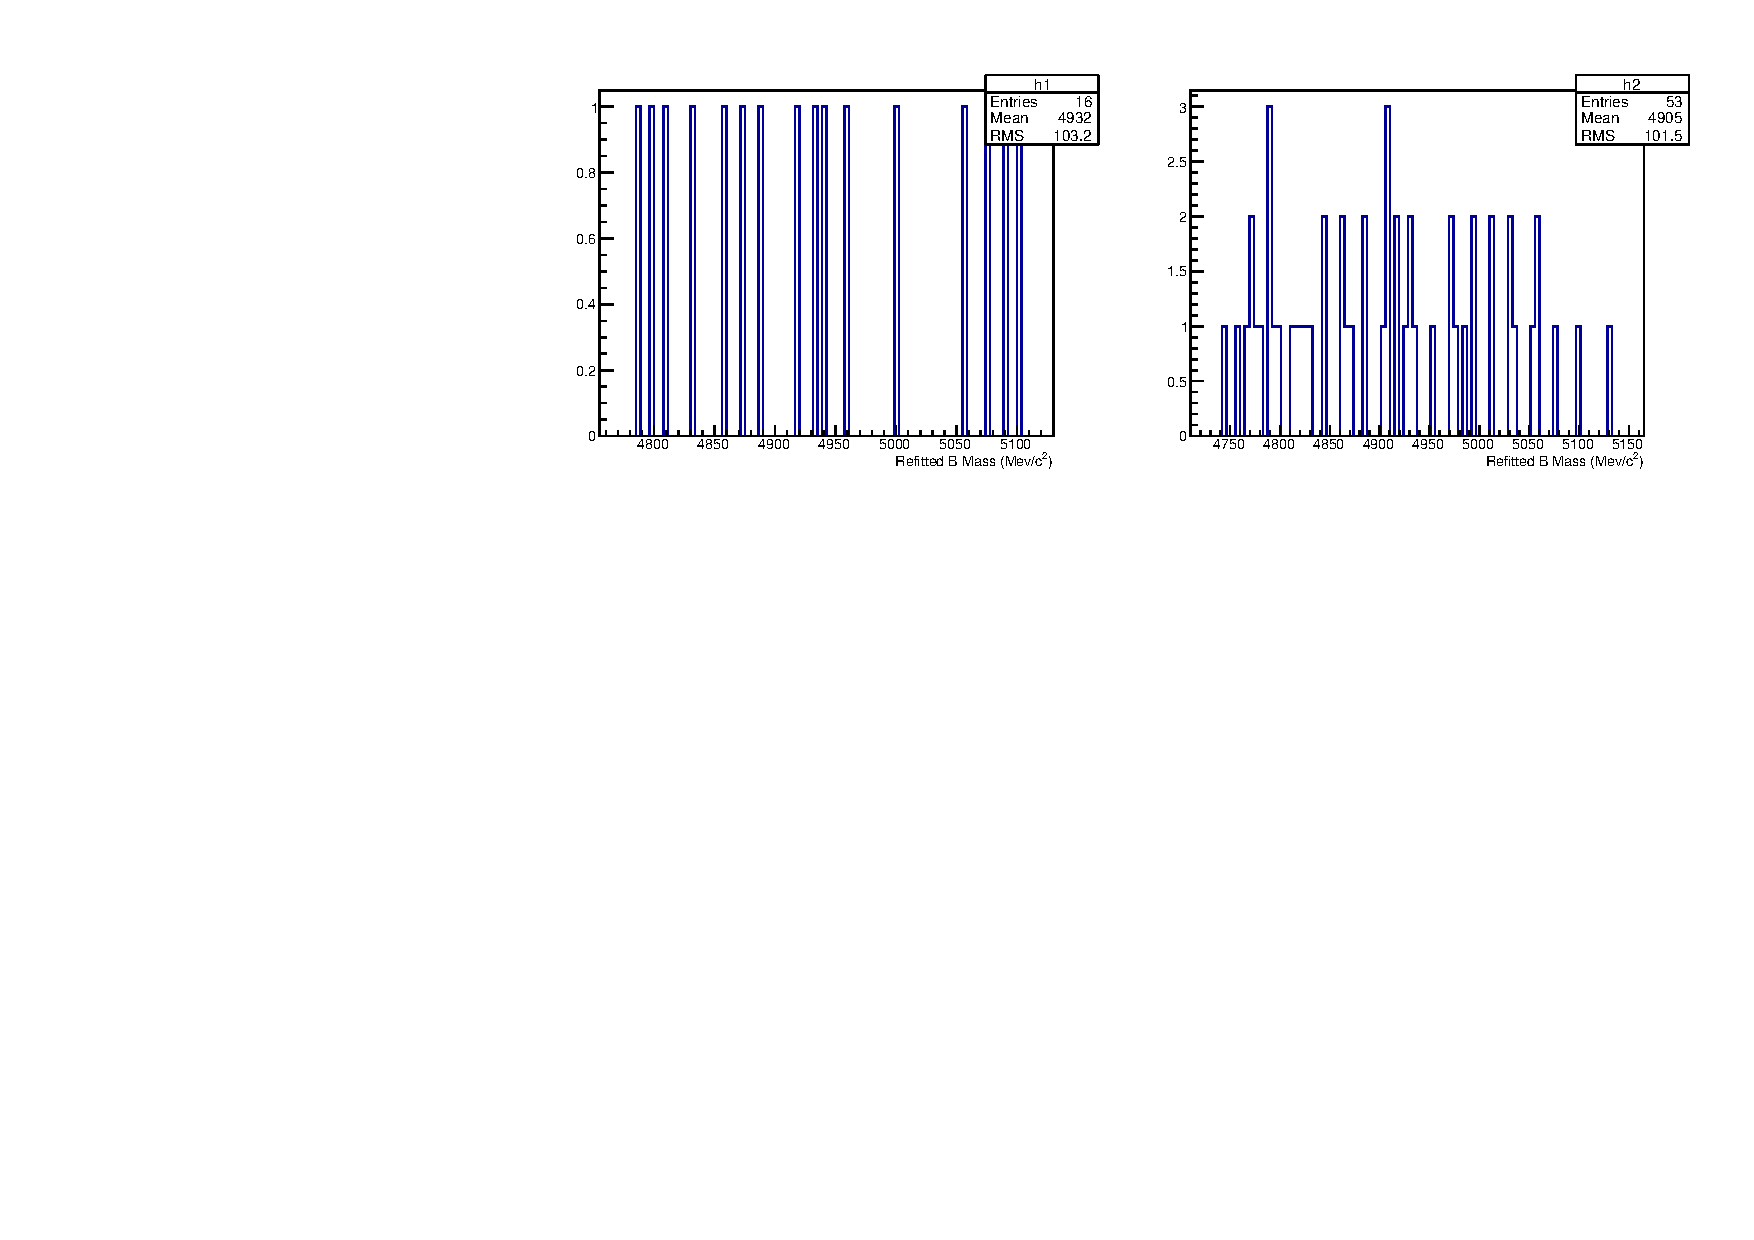
\includegraphics[width=0.7\linewidth]{figures/backgrounds/B2DKstPi0.pdf}
\caption{\decay{\B}{\D\Kstar\piz} MC events remaining after the full selection is applied to 1M generated events}
\label{B2DKstPi0}
\end{figure}

\subsubsection{\decay{\B}{\D\KS\kaon}}

The decay \decay{\B}{\D\KS\kaon} has a branching fraction of $5.5 \times 10^{-4}$~\cite{PDG2014}. Figure \ref{B2DKKs} shows the remaining events after applying the full selection to 1M \decay{\B}{\D\KS\kaon} MC events. The estimated contribution in the favoured \decay{\B}{\D(\kaon\pi)\Kstar} mass fit is 0.5\% and 0.4\%, for LL and DD respectively, of the signal in the mass range 4900-5250 MeV. The low mass range for the simultaneous fit is 5230 MeV and so this background is considered negligible.

\begin{figure}[h]
\centering
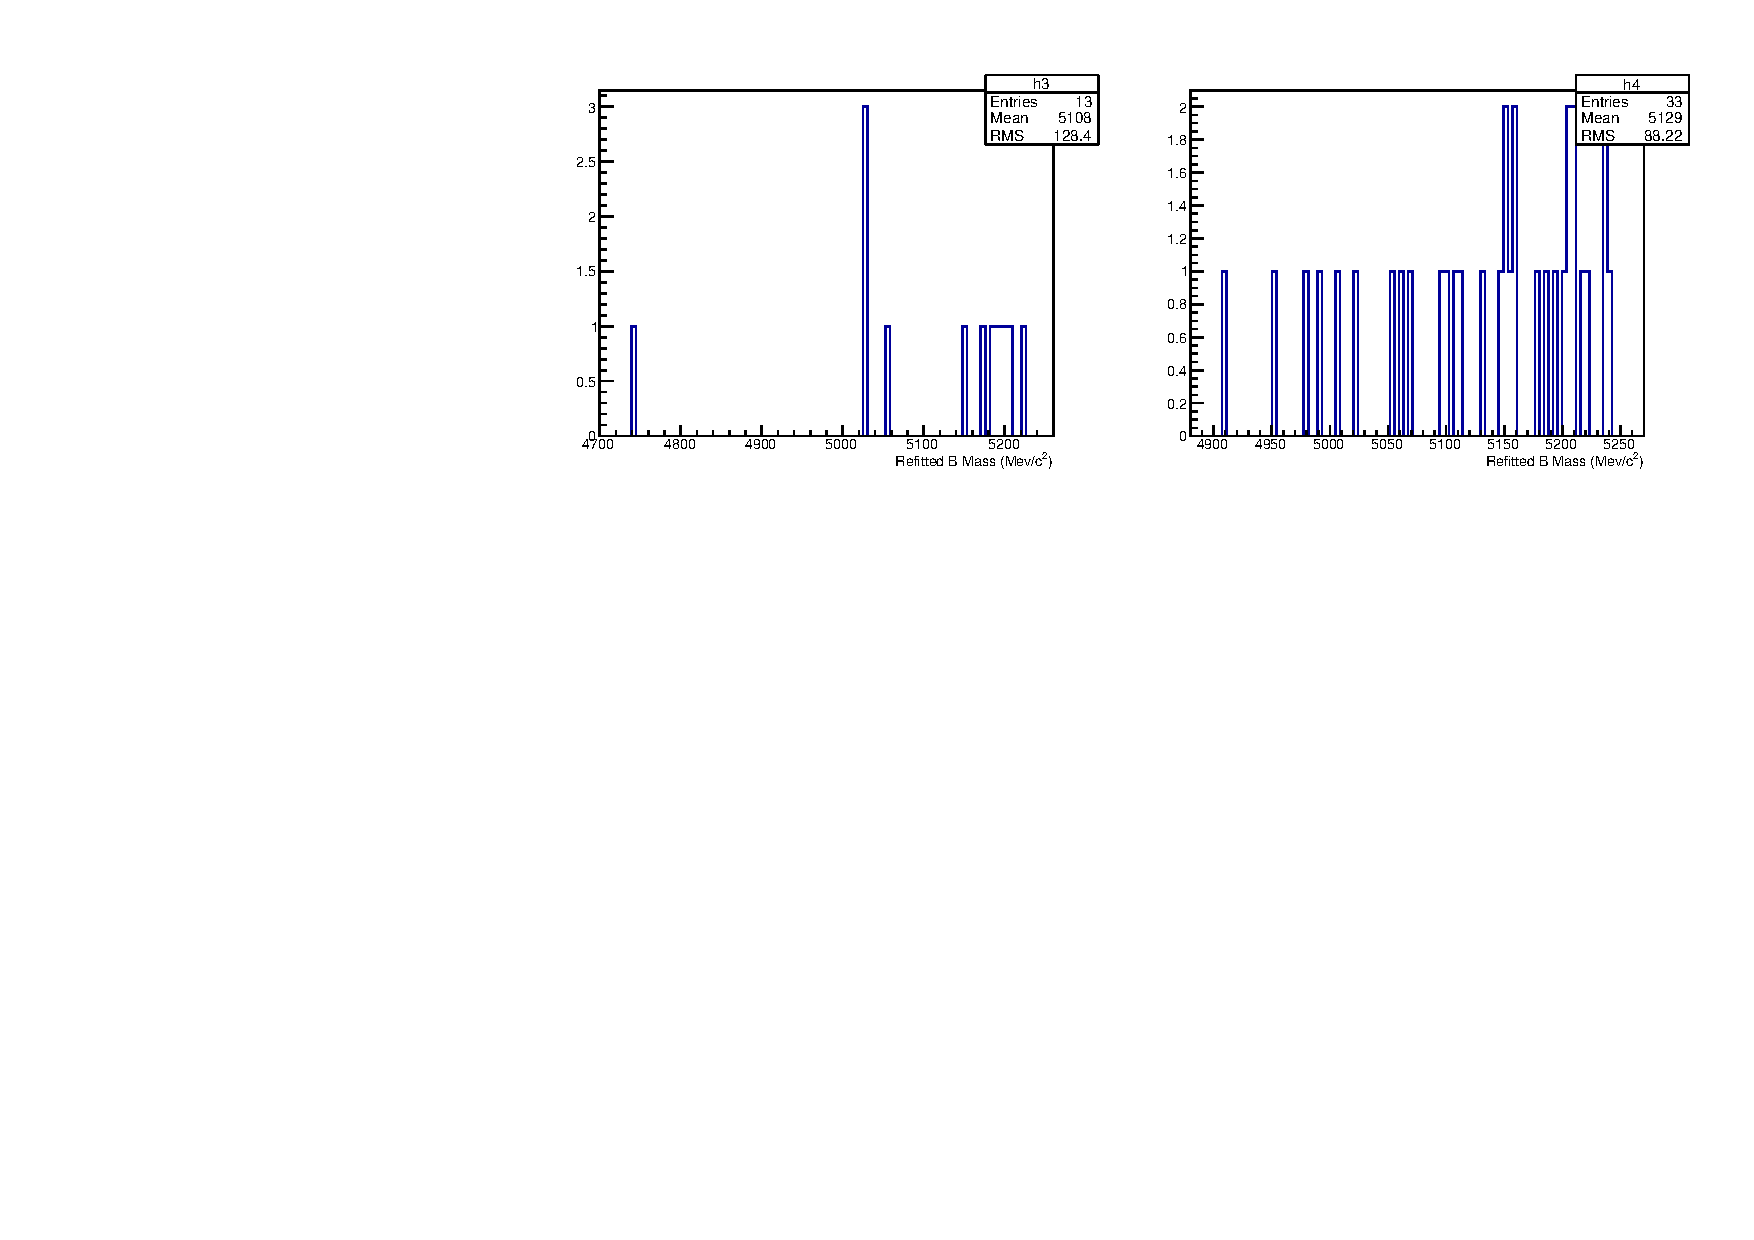
\includegraphics[width=0.7\linewidth]{figures/backgrounds/B2DKKs.pdf}
\caption{\decay{\B}{\D\KS\kaon} MC events remaining after the full selection is applied to 1M generated events}
\label{B2DKKs}
\end{figure}

\subsubsection{\decay{\Bs}{\Dz\KS\pi\pi}}

There is no measured branching fraction for \decay{\Bs}{\Dz\KS\pi\pi}. A \decay{\Bs}{\Dz\KS\pi\pi} branching fraction of $5 \times 10^{-4}$ is assumed. The full selection is applied to 0.5M \decay{\Bs}{\Dz\KS\pi\pi} events, Figure \ref{Bs2D0KsPiPi} shows the distribution of the remaining events. The estimated contribution in the favoured \decay{\B}{\D(\kaon\pi)\Kstar} mass fit is 0.4\% and 0.2\% of the signal, for LL and DD respectively, across the mass range 4750-5120 MeV. As the simultaneous fit has a mass range starting from 5230 MeV, this background is not considered for the mass fit.

\begin{figure}[h]
\centering
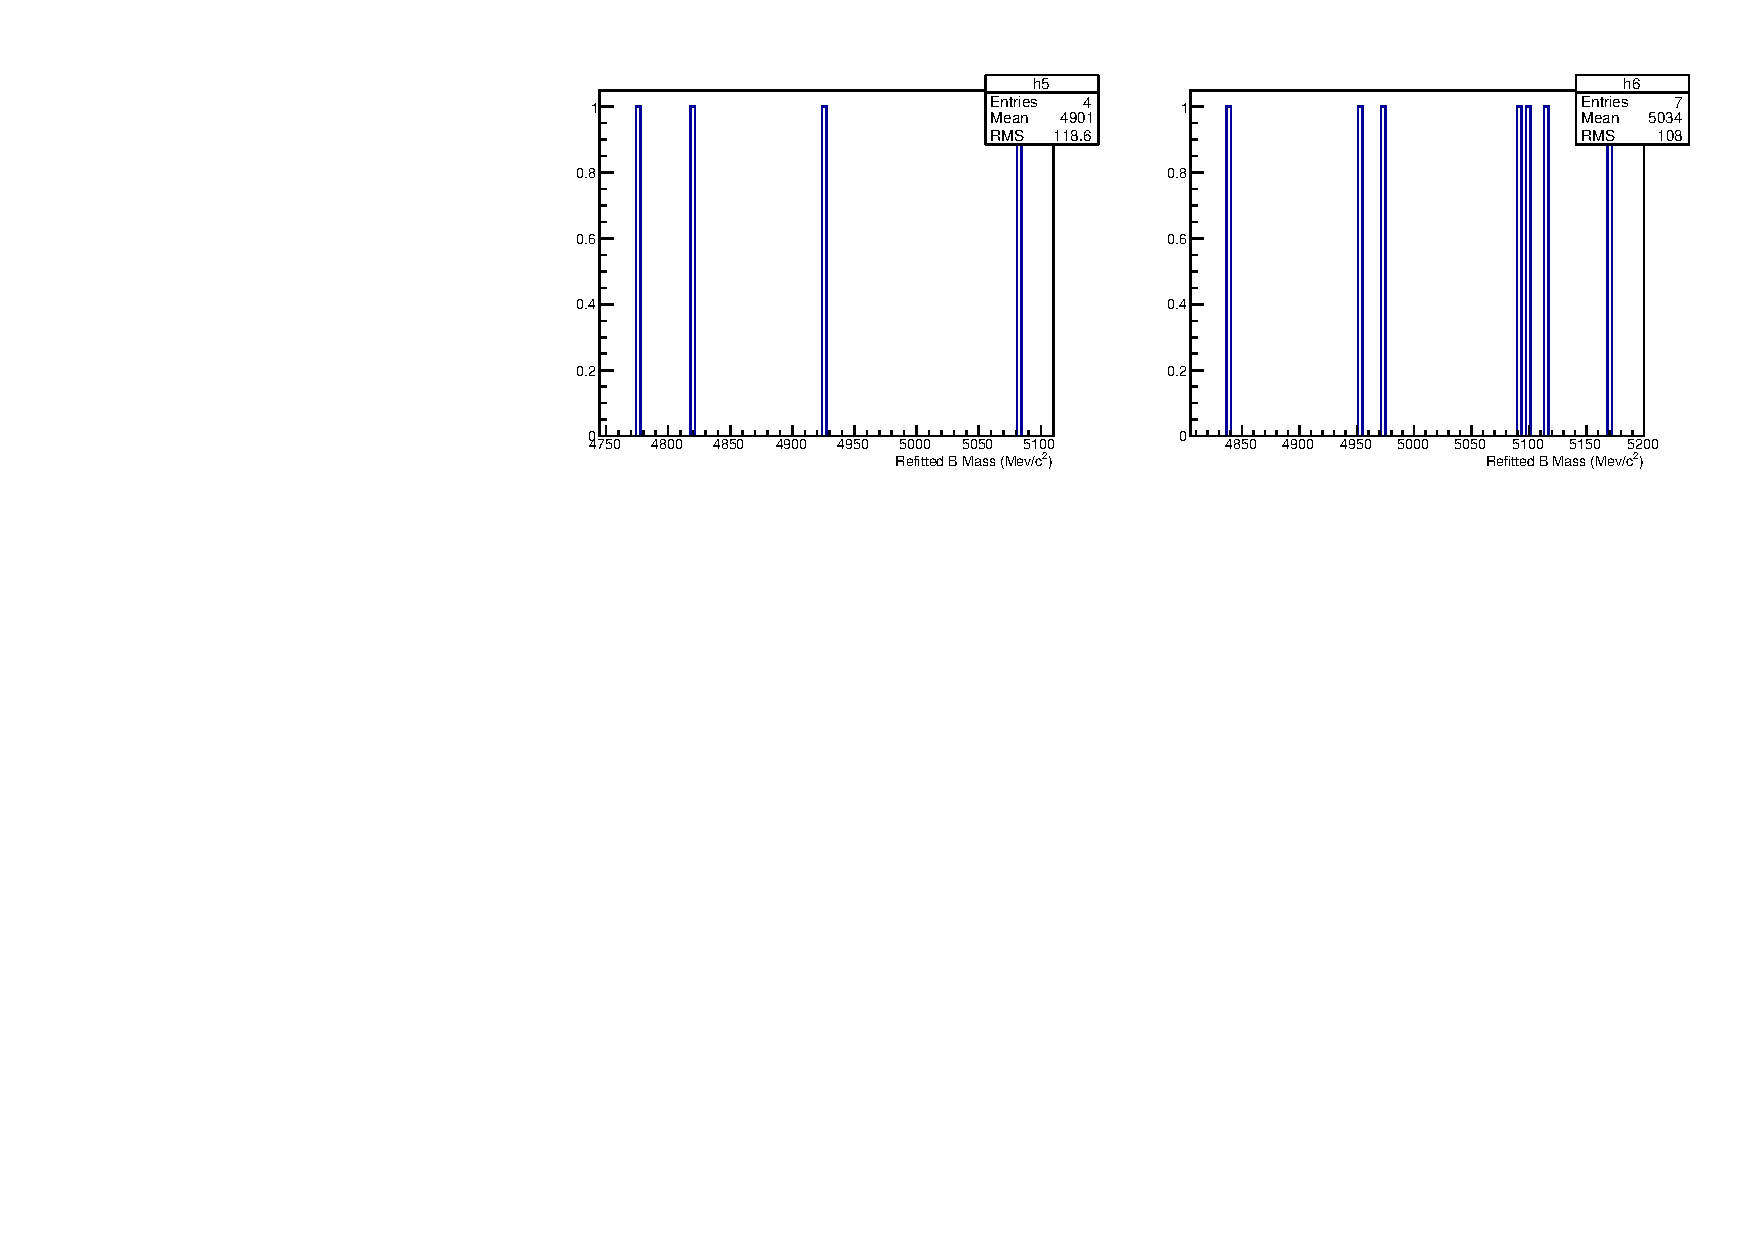
\includegraphics[width=0.7\linewidth]{figures/backgrounds/Bs2D0KsPiPi.pdf}
\caption{\decay{\Bs}{\Dz\KS\pi\pi} MC events remaining after the full selection is applied to 1M generated events}
\label{Bs2D0KsPiPi}
\end{figure}

\clearpage

\section{Simultaneous fit plot with log scale}
\label{app:sec:logscale}

\begin{sidewaysfigure}[h]
\centering
\subfloat[$K\pi$, LL]{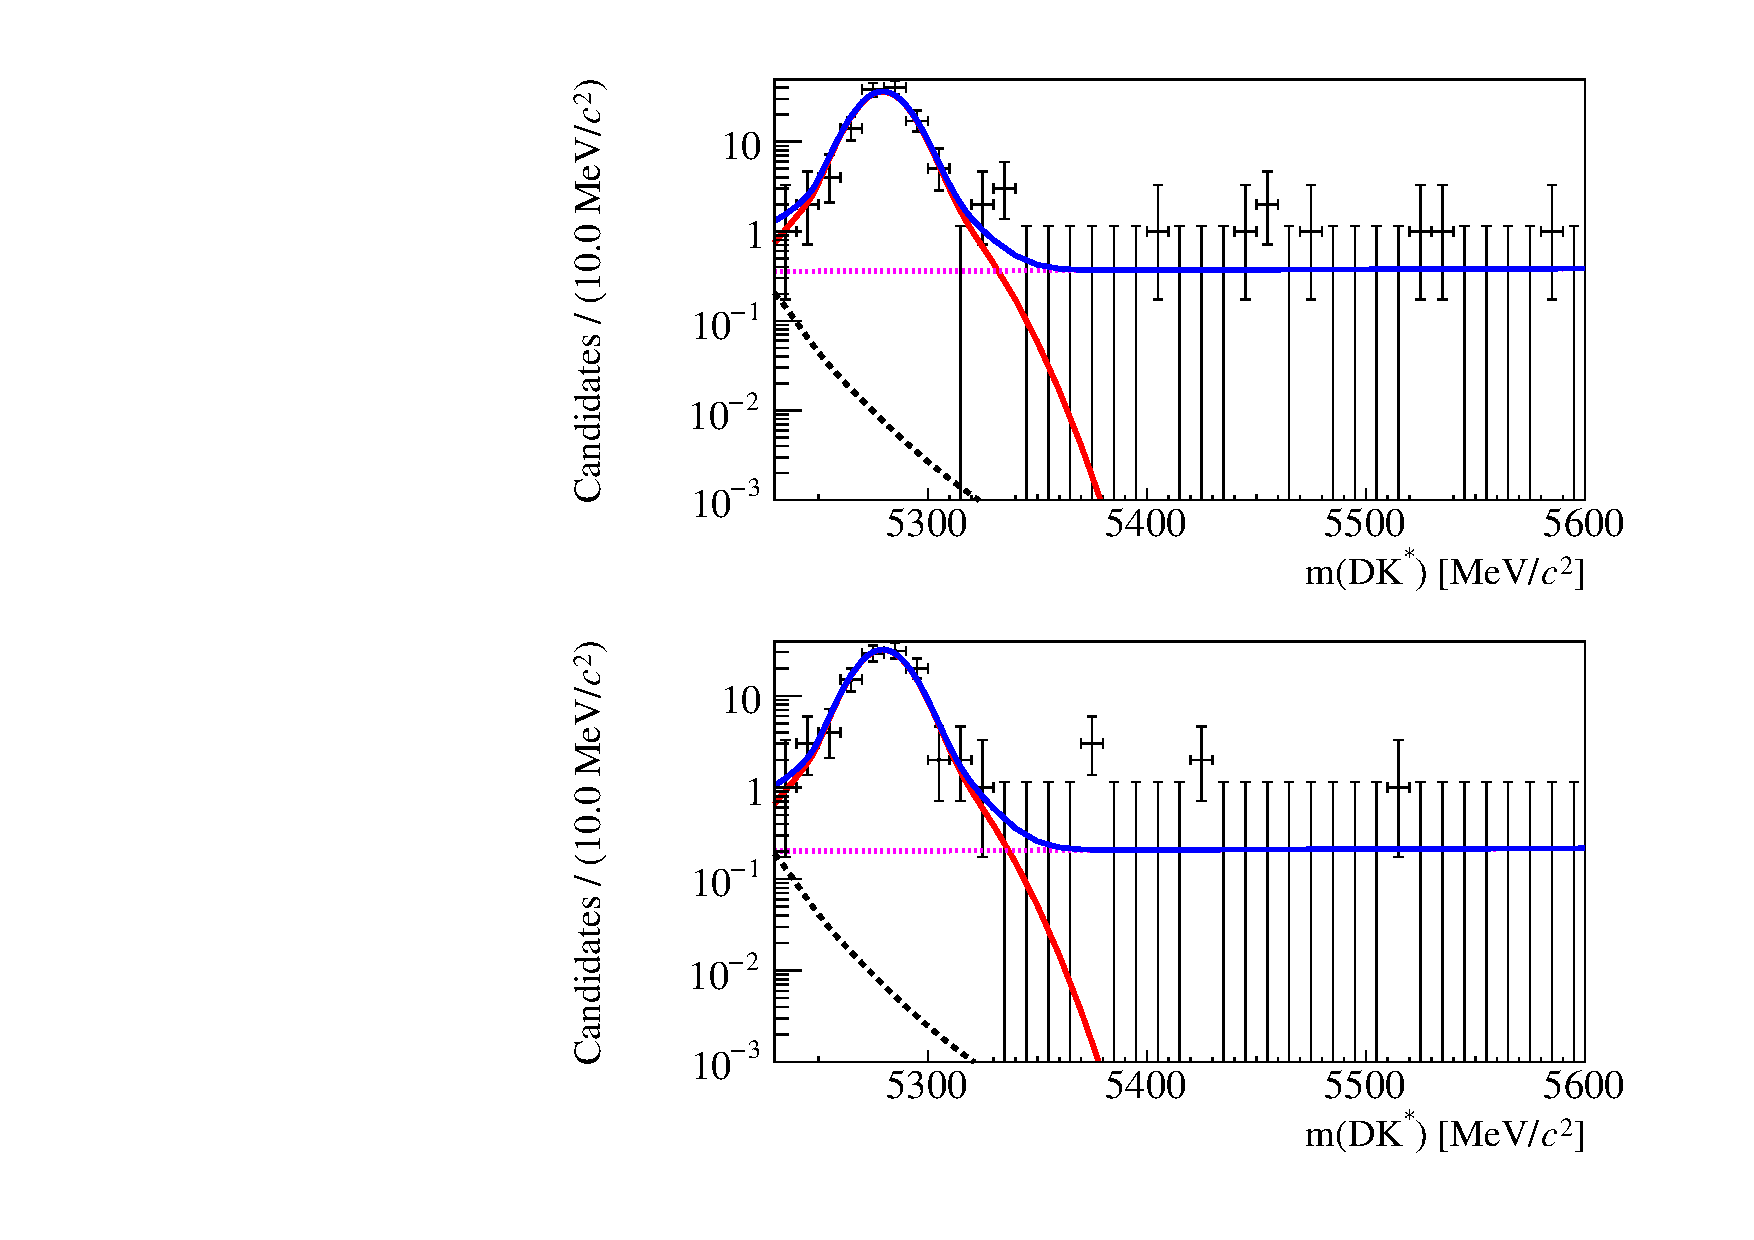
\includegraphics[width=0.25\linewidth]{figures/results/canvaslog_d2kpi_LL_run1_log.pdf}}
\hfill
\subfloat[$KK$, LL]{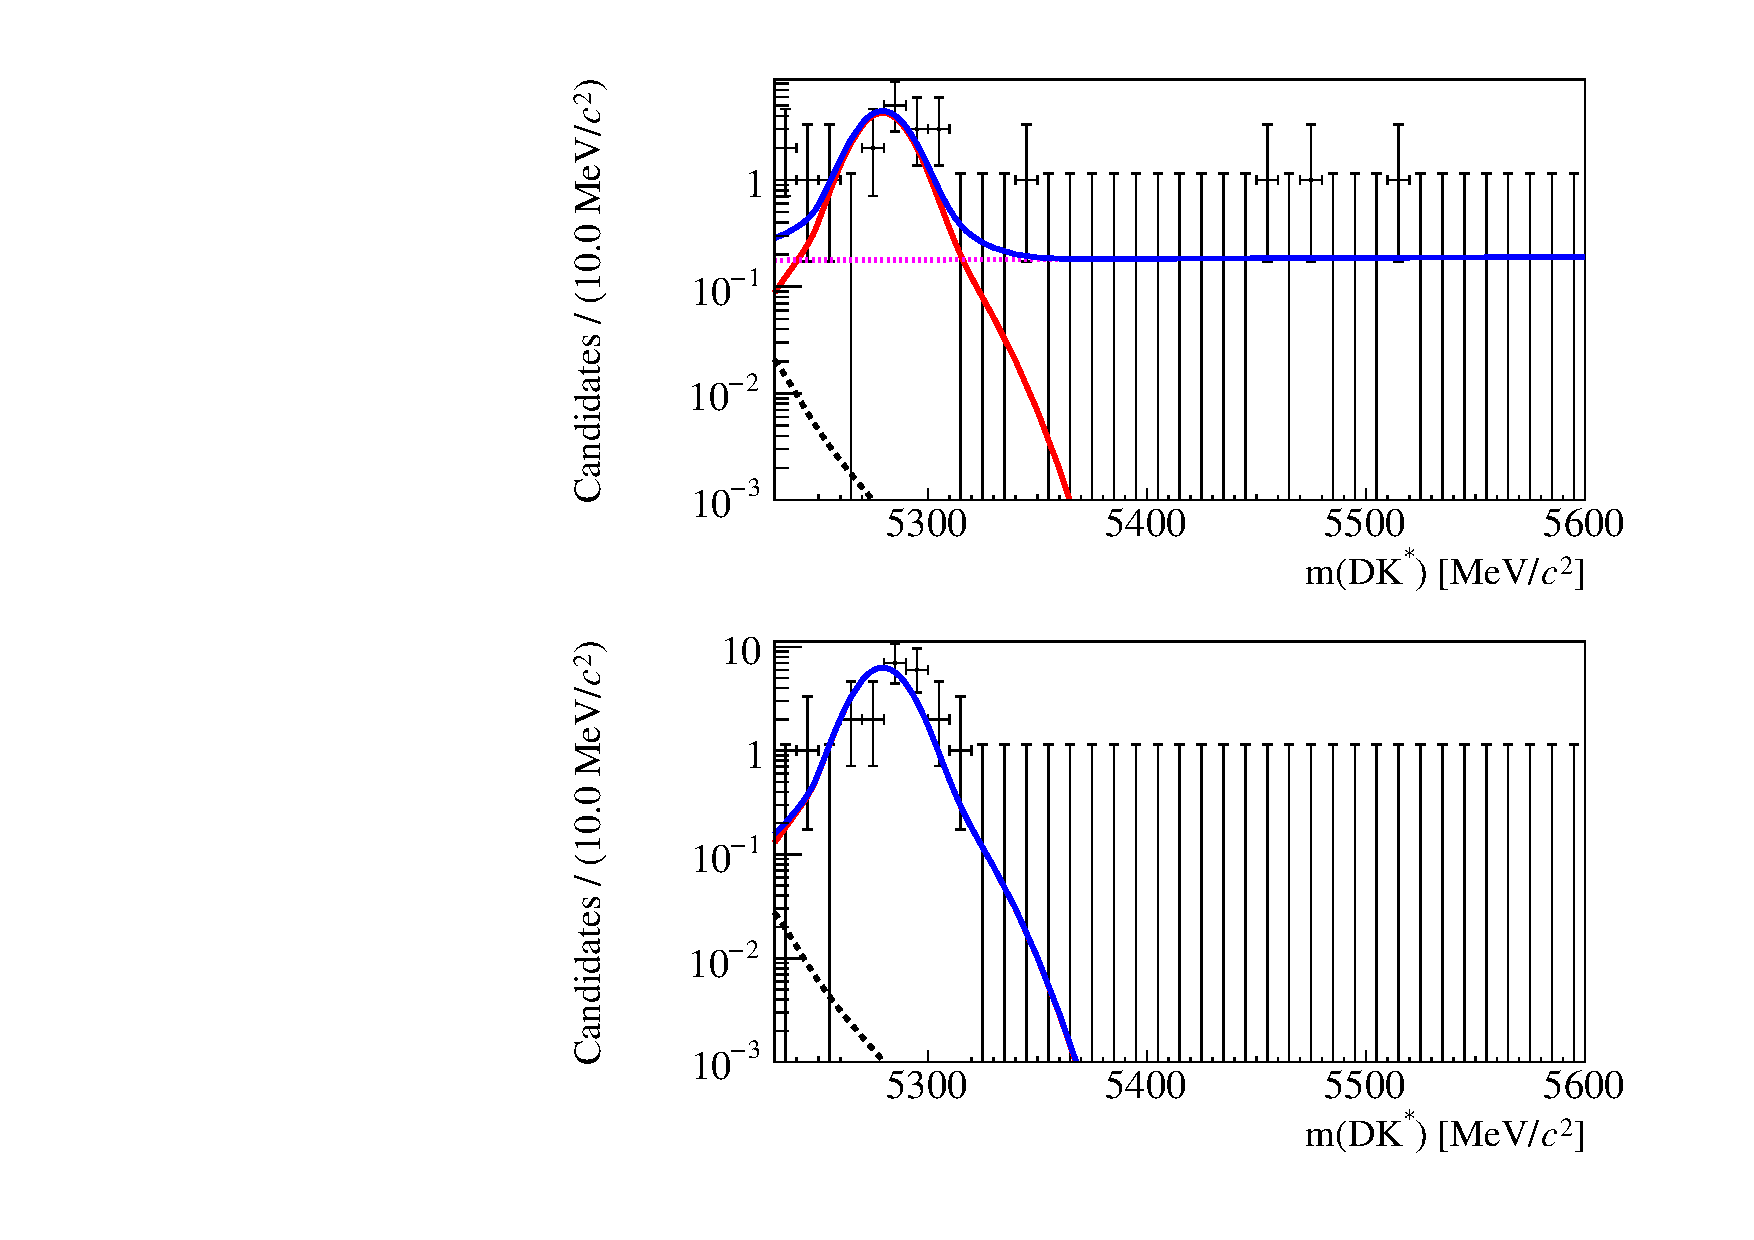
\includegraphics[width=0.25\linewidth]{figures/results/canvaslog_d2kk_LL_run1_log.pdf}}
\hfill
\subfloat[$\pi\pi$, LL]{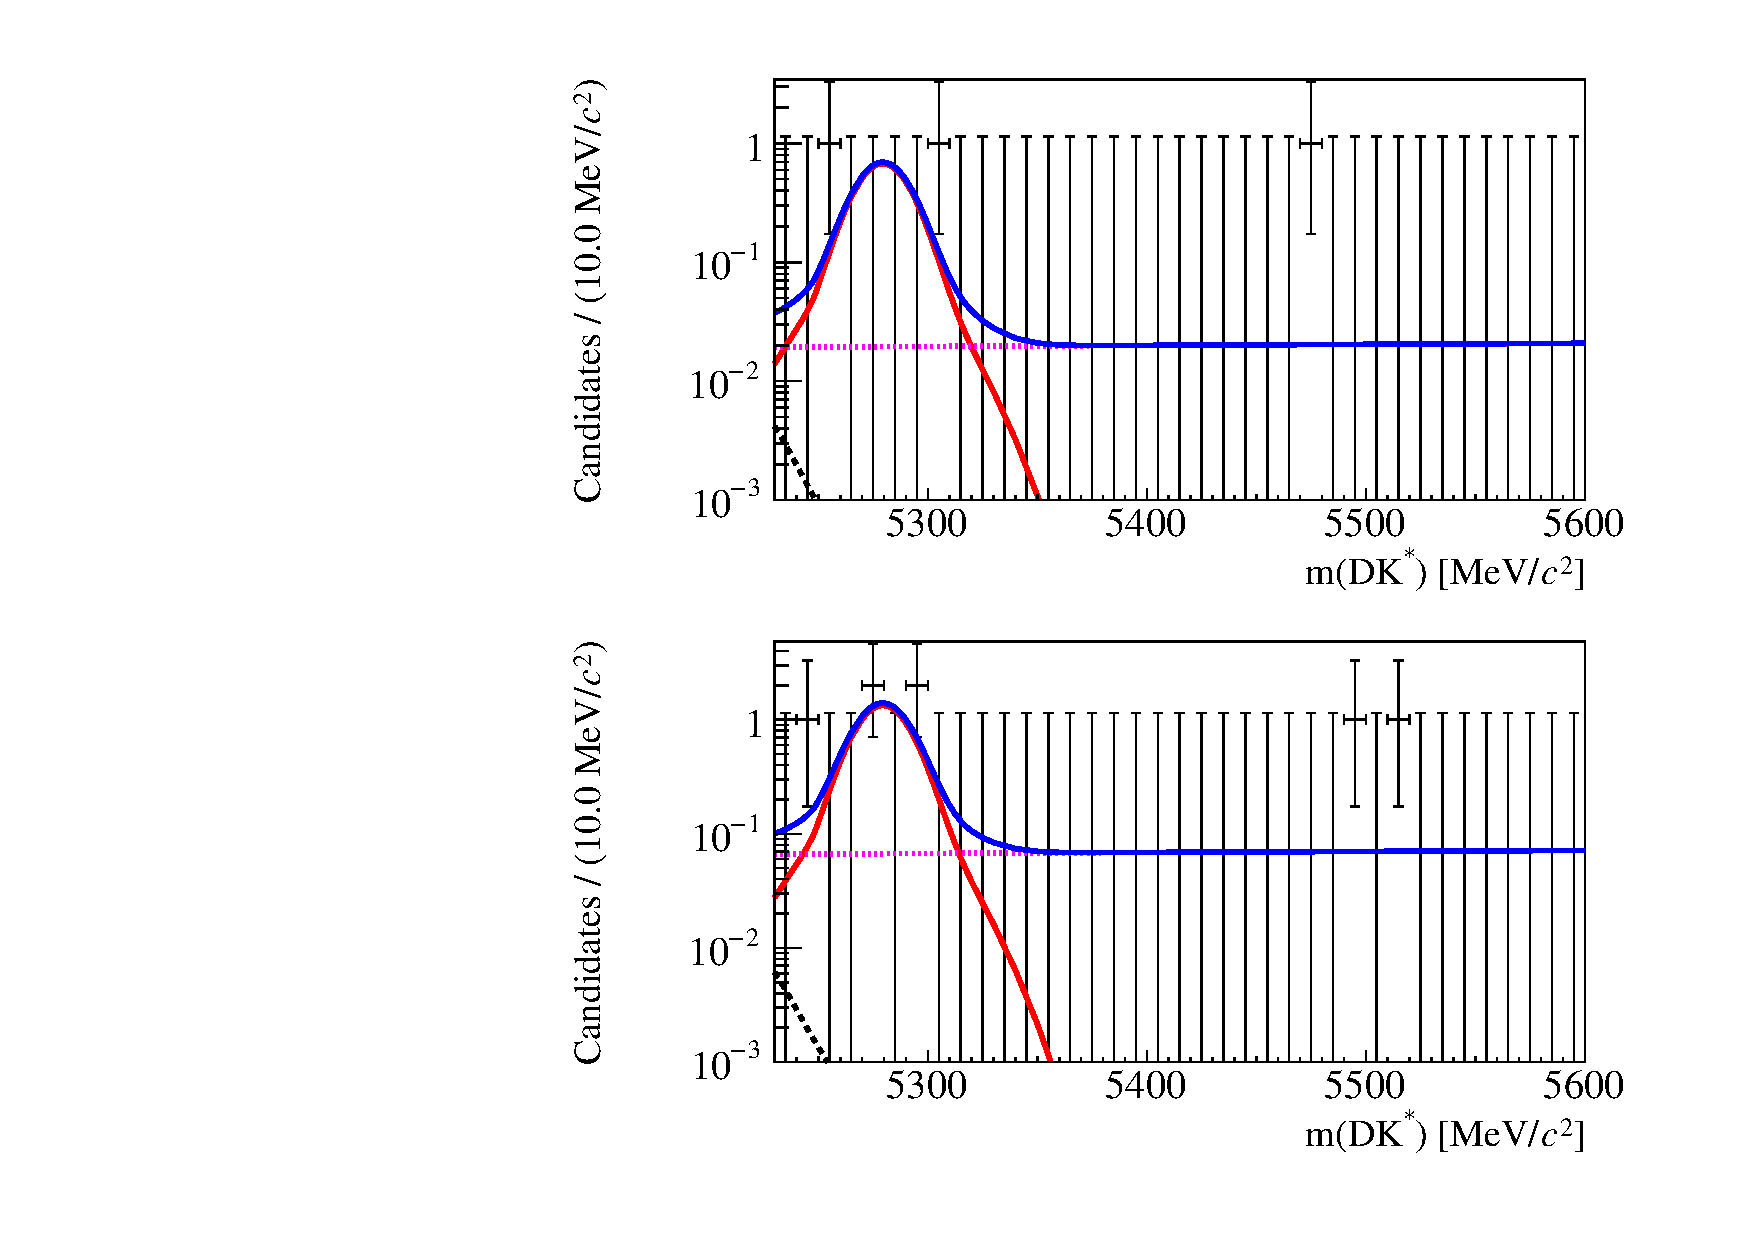
\includegraphics[width=0.25\linewidth]{figures/results/canvaslog_d2pipi_LL_run1_log.pdf}}
\hfill
\subfloat[$\pi K$, LL]{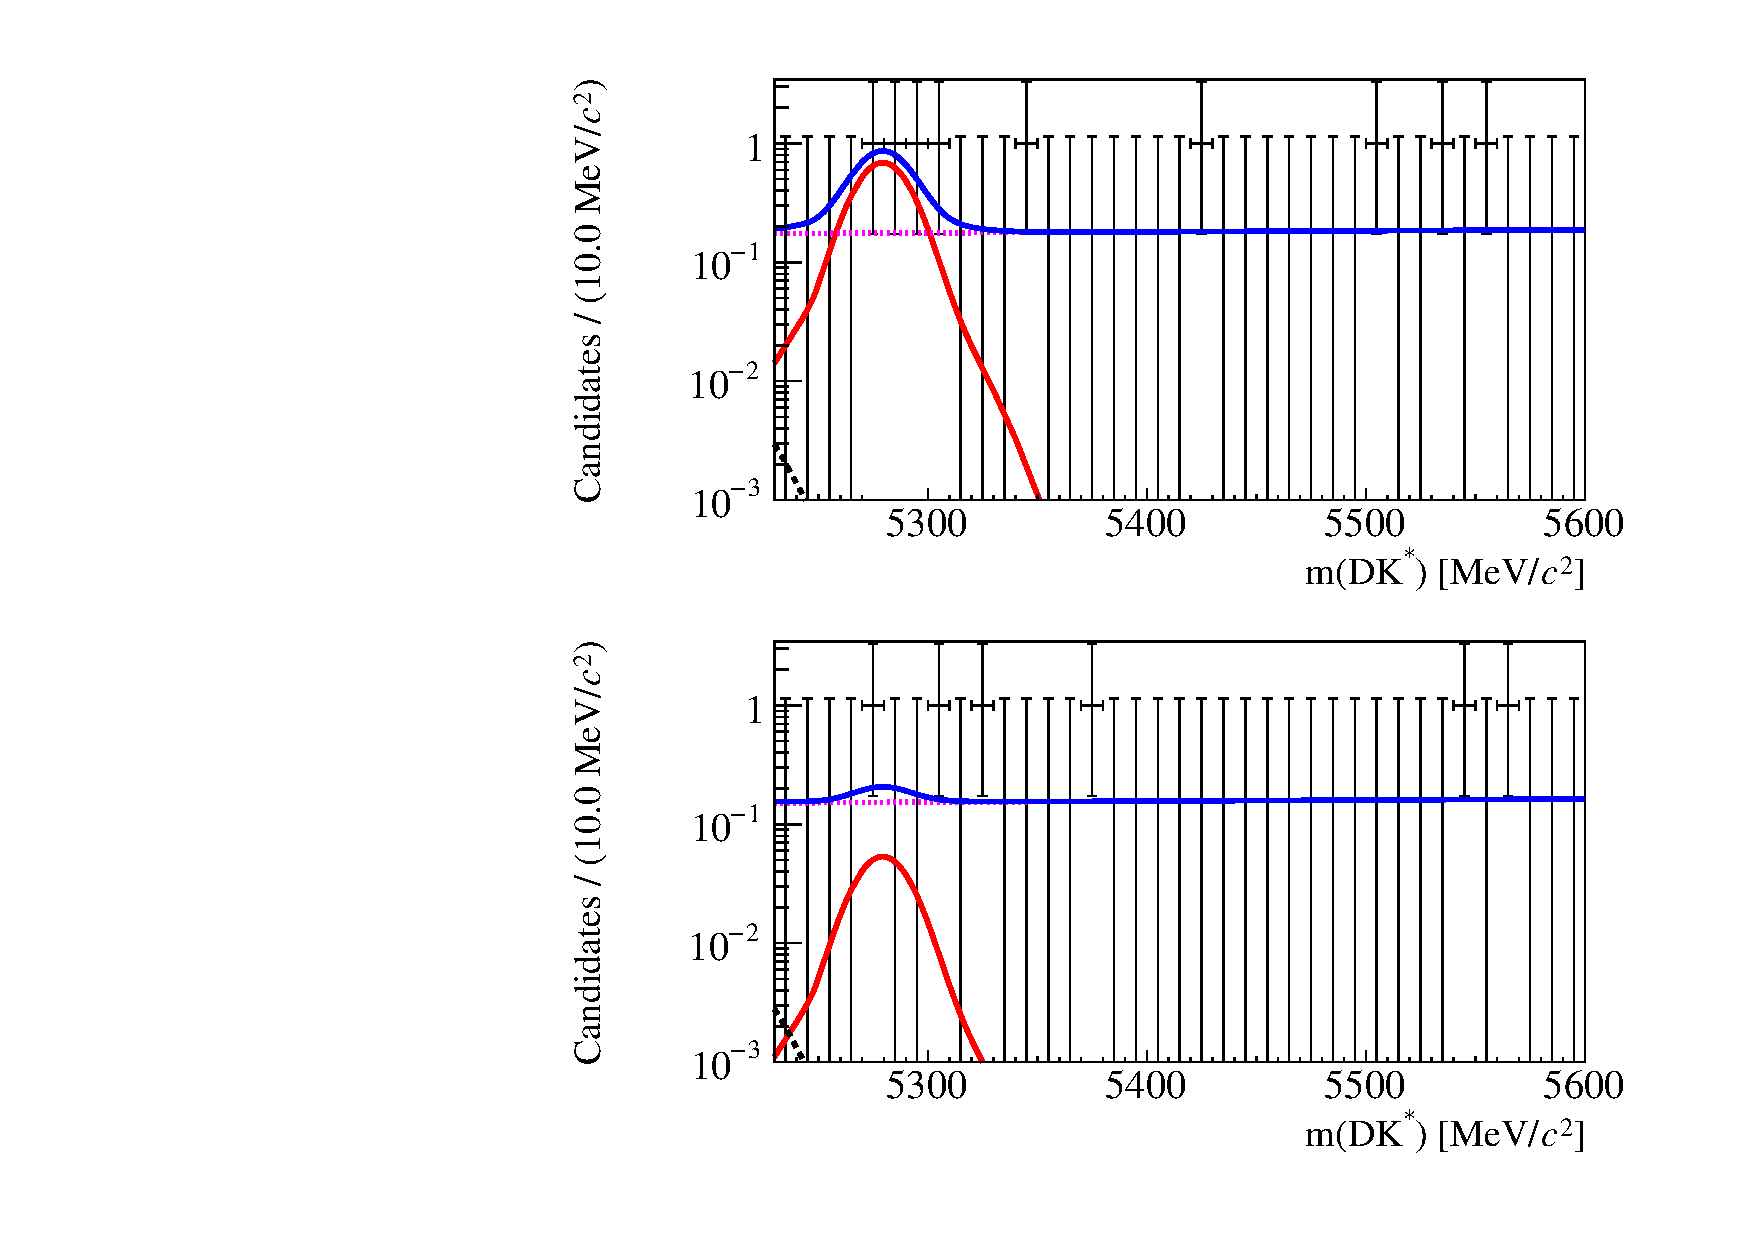
\includegraphics[width=0.25\linewidth]{figures/results/canvaslog_d2pik_LL_run1_log.pdf}}
\hfill
\subfloat[$K\pi$, DD]{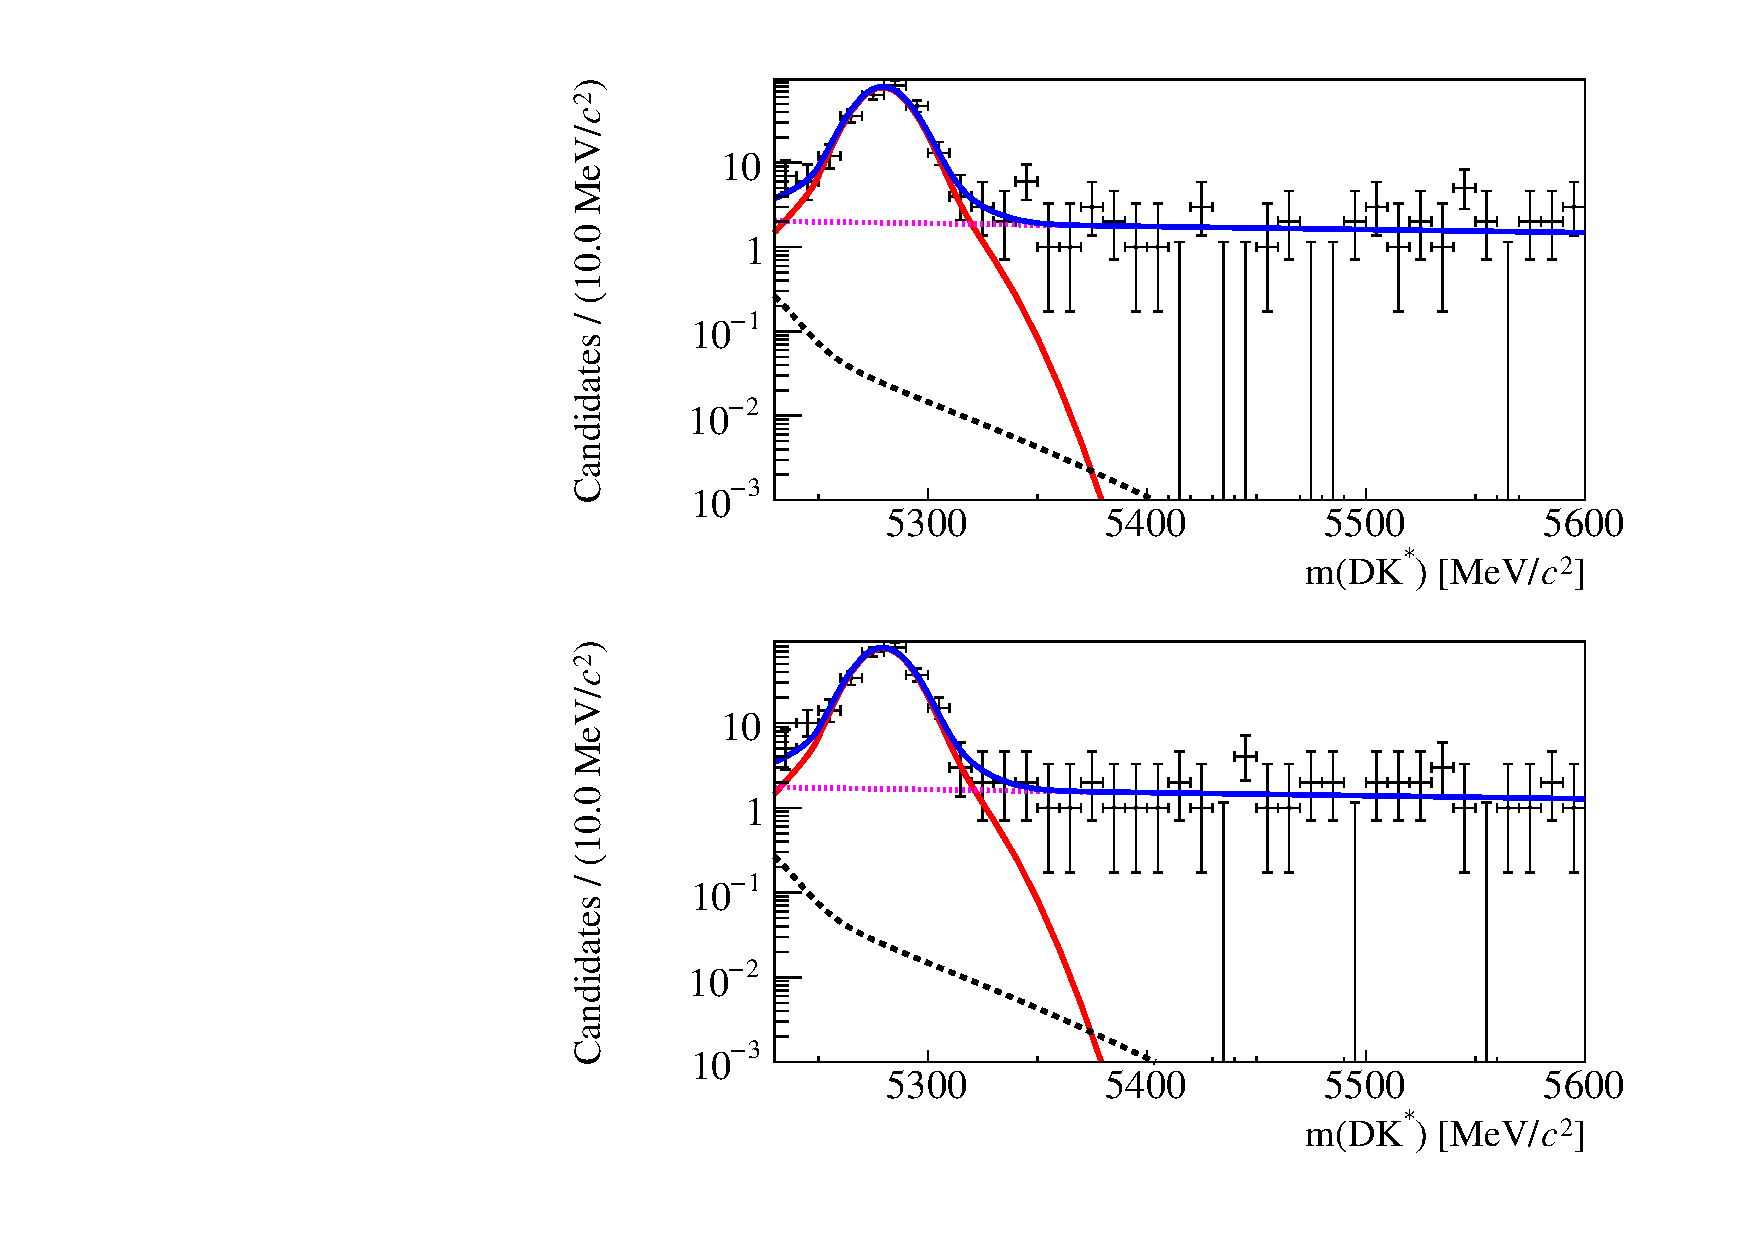
\includegraphics[width=0.25\linewidth]{figures/results/canvaslog_d2kpi_DD_run1_log.pdf}}
\hfill
\subfloat[$KK$, DD]{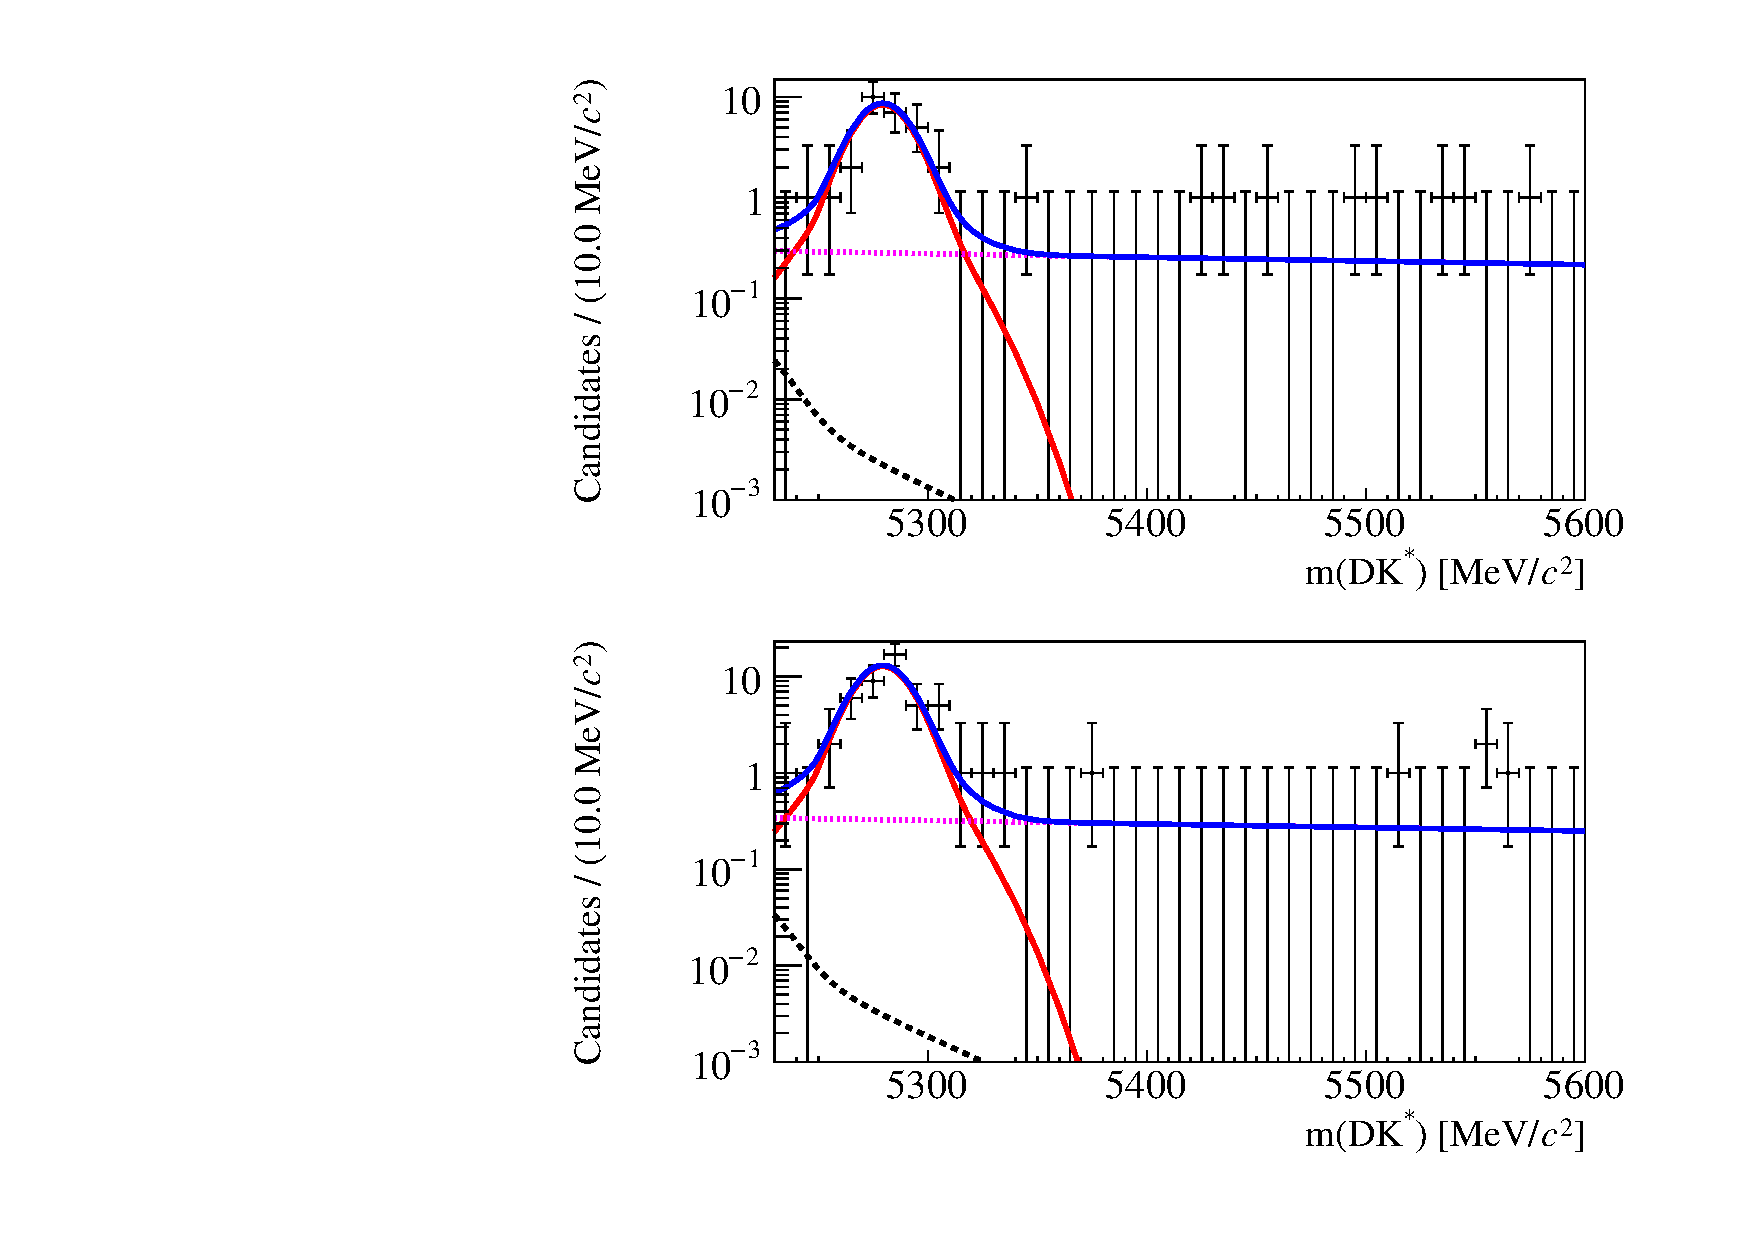
\includegraphics[width=0.25\linewidth]{figures/results/canvaslog_d2kk_DD_run1_log.pdf}}
\hfill
\subfloat[$\pi\pi$, DD]{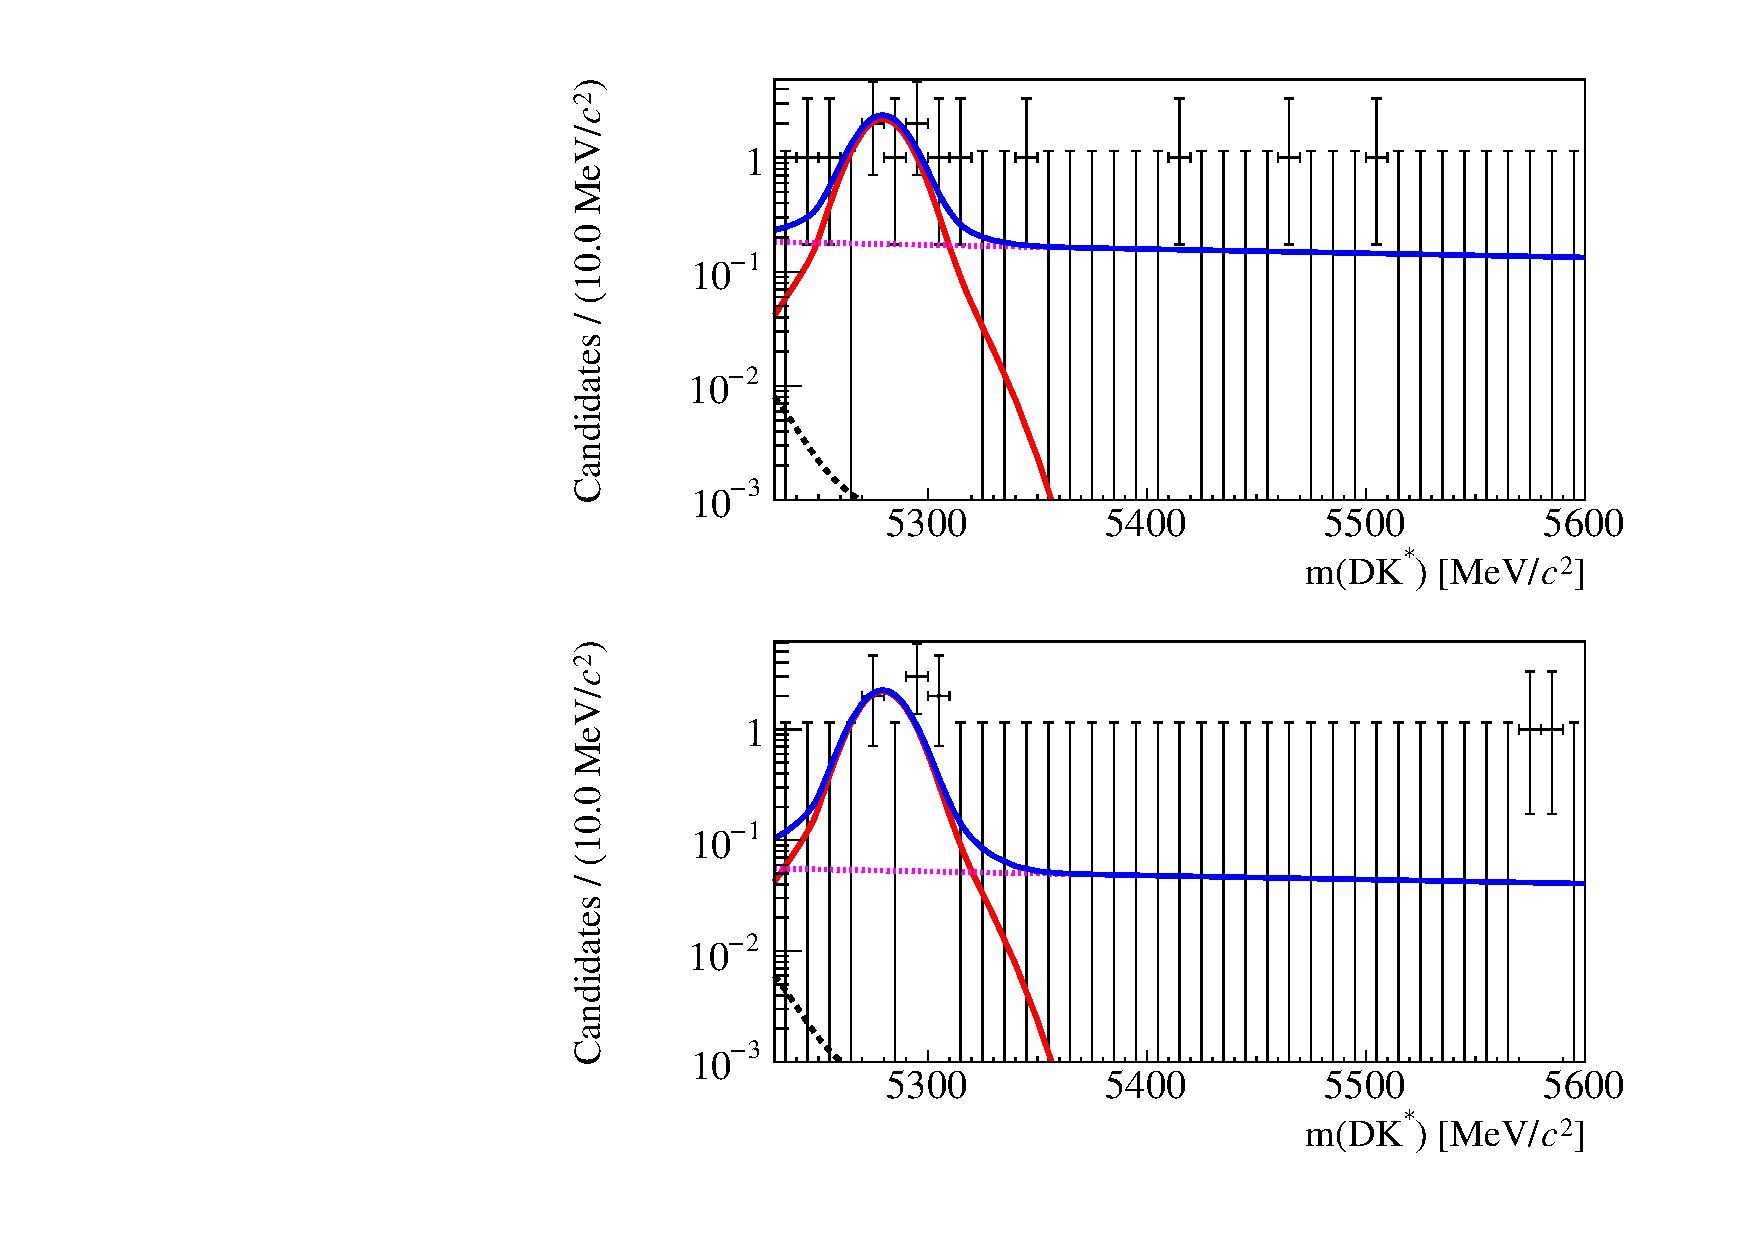
\includegraphics[width=0.25\linewidth]{figures/results/canvaslog_d2pipi_DD_run1_log.pdf}}
\hfill
\subfloat[$\pi K$, DD]{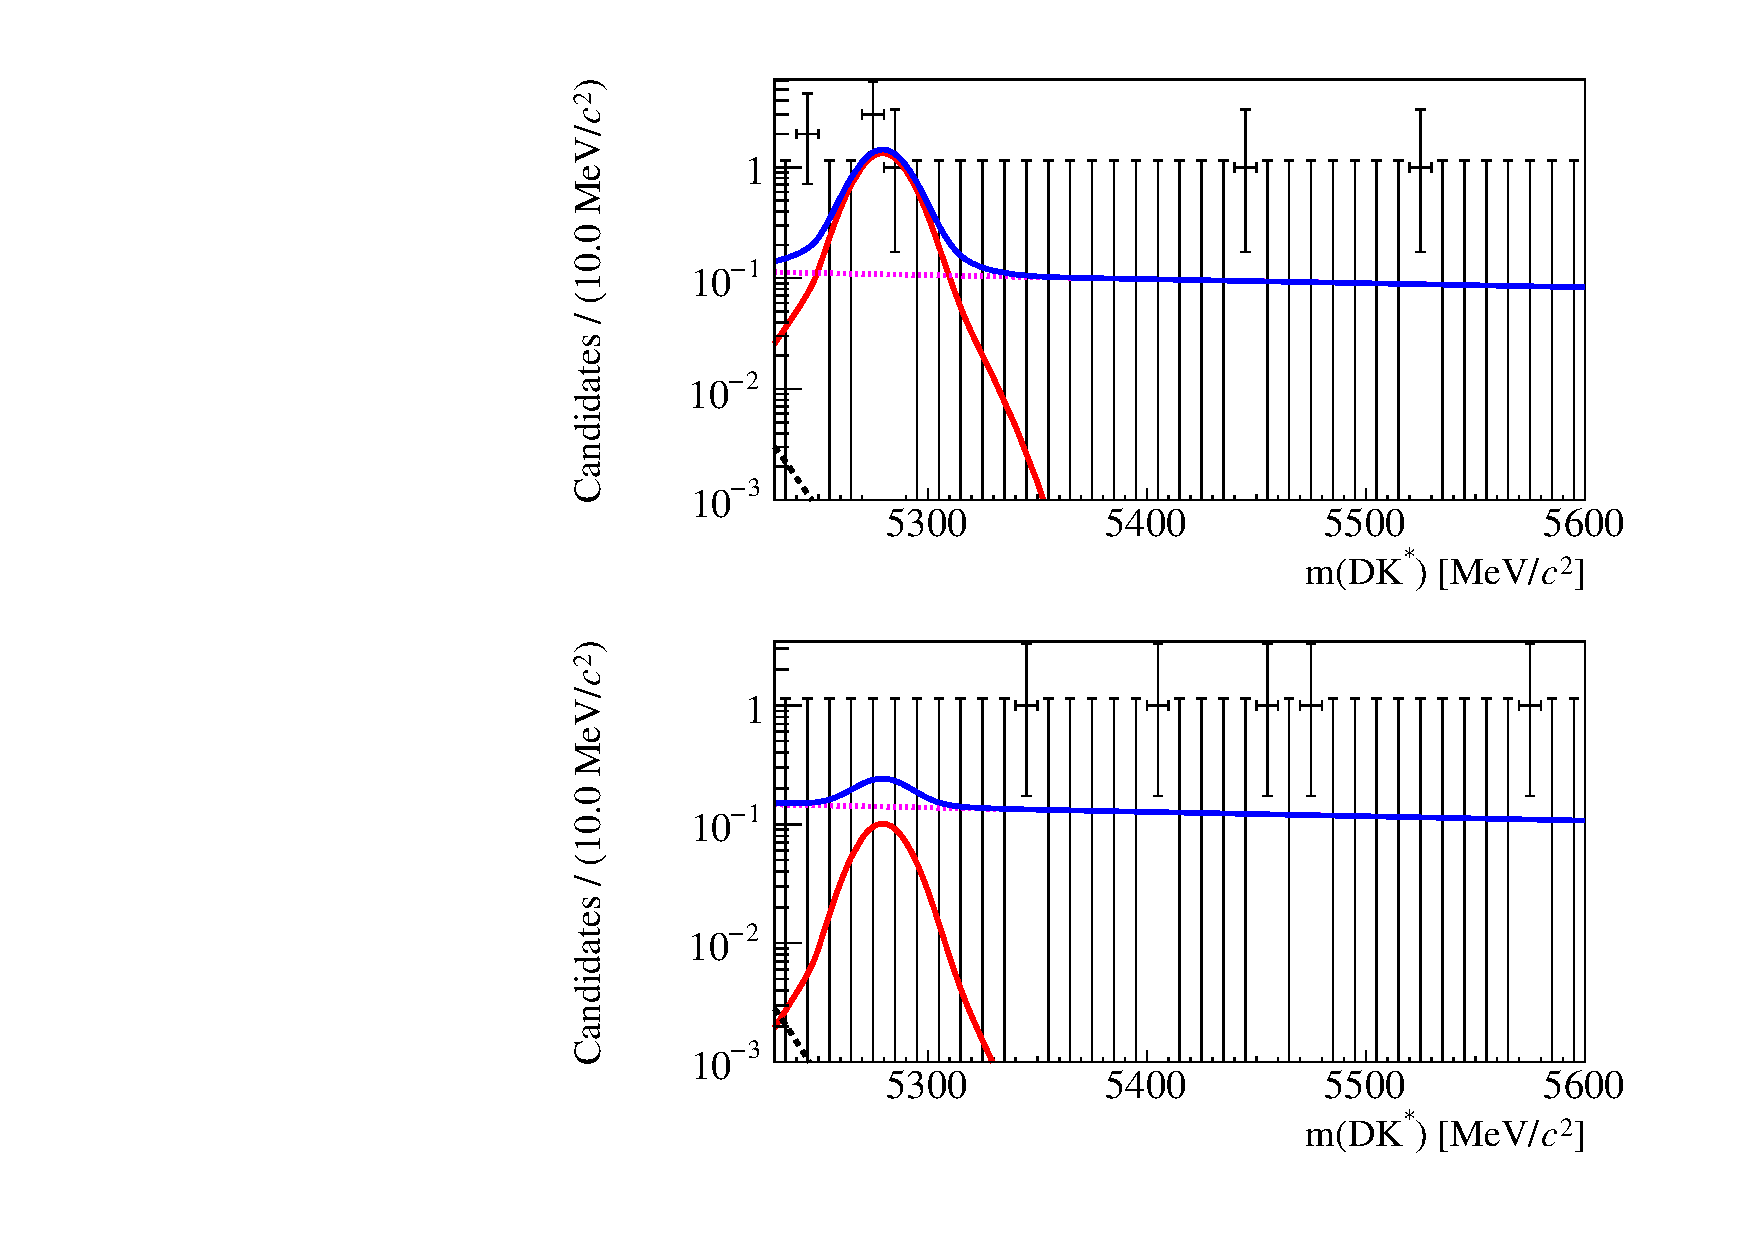
\includegraphics[width=0.25\linewidth]{figures/results/canvaslog_d2pik_DD_run1_log.pdf}}
\caption{Results of the simultaneous fit for Run 1 data for 2-body modes. In each pair the top plot is for \Bp decays and the bottom plot is for \Bm decays.}
\label{datafit2bodyRun1}
\end{sidewaysfigure}

\begin{sidewaysfigure}[h]
\centering
\subfloat[$K\pi\pi\pi$, LL]{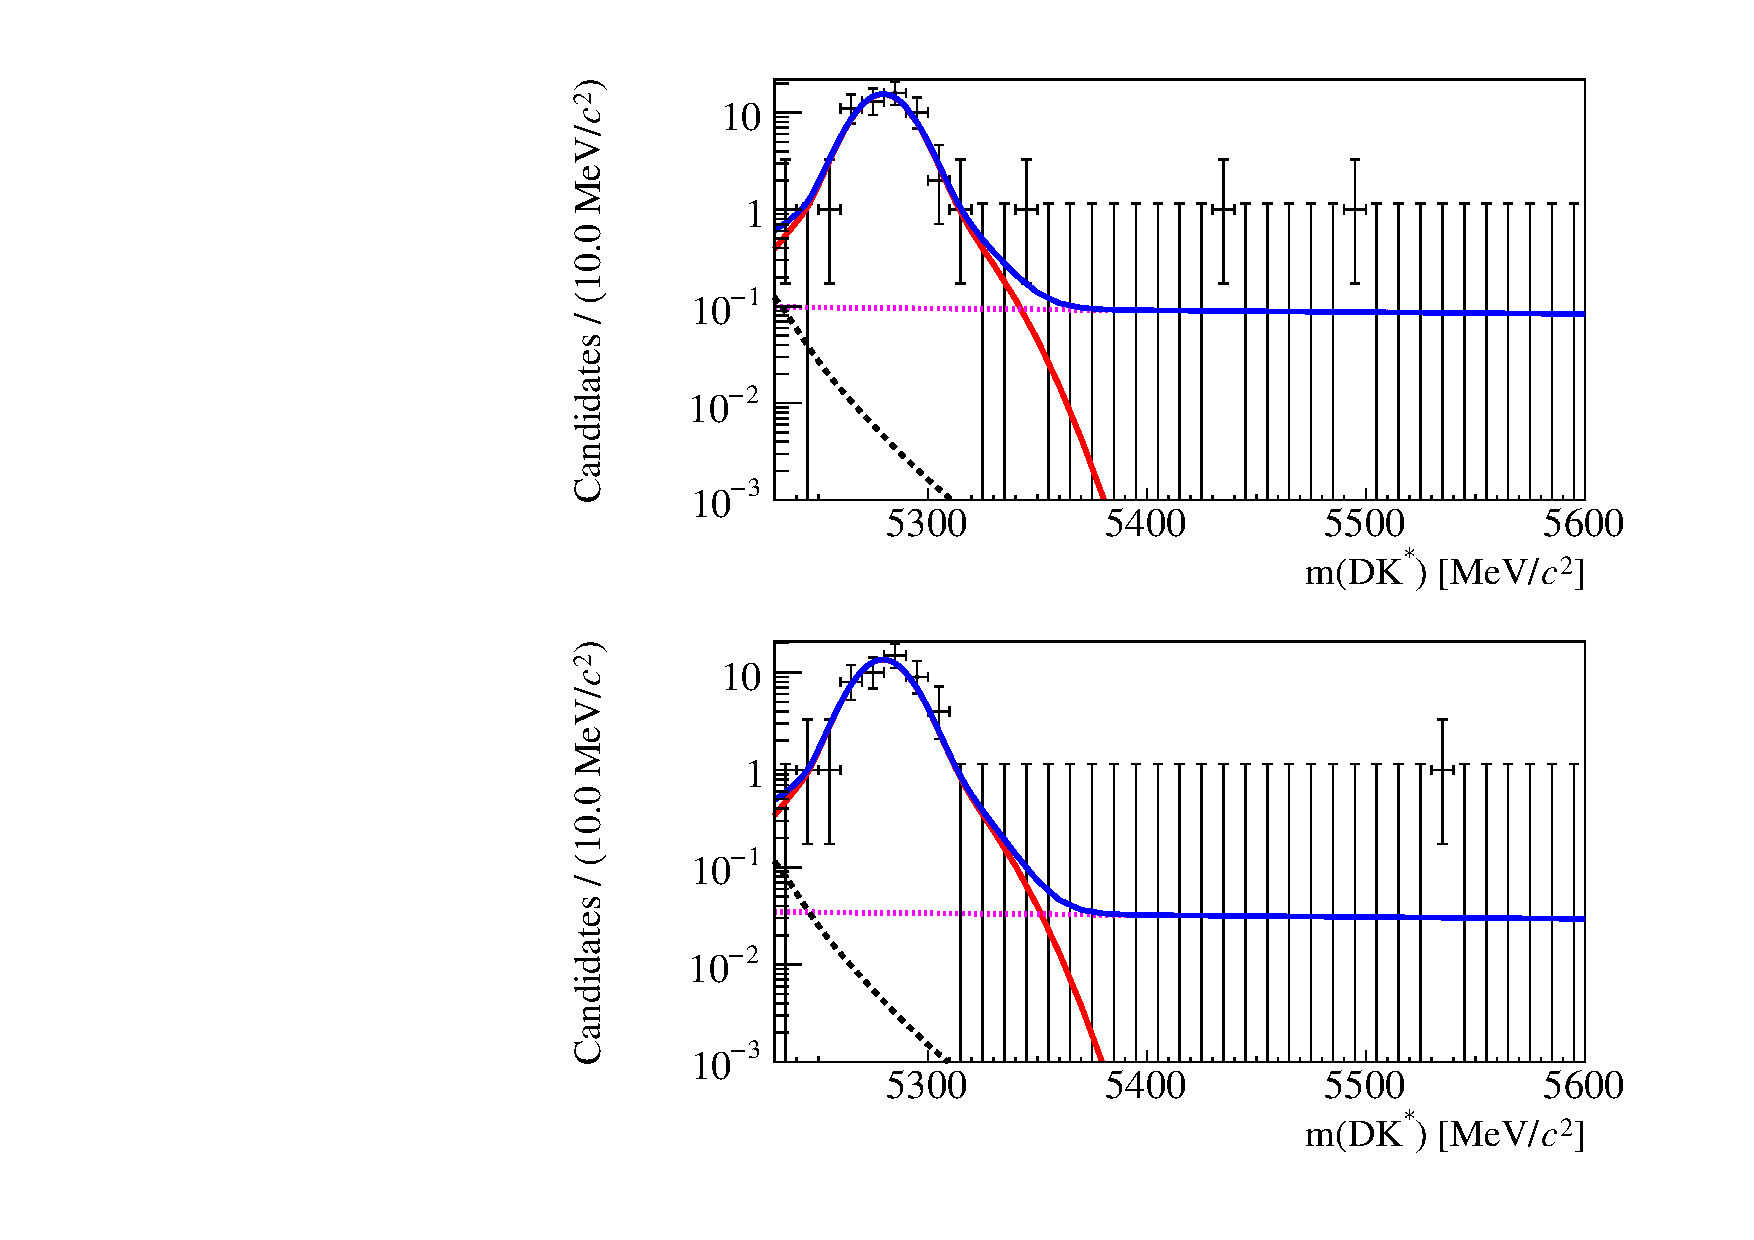
\includegraphics[width=0.3\linewidth]{figures/results/canvaslog_d2kpipipi_LL_run1_log.pdf}}
\hfill
\subfloat[$\pi\pi\pi\pi$, LL]{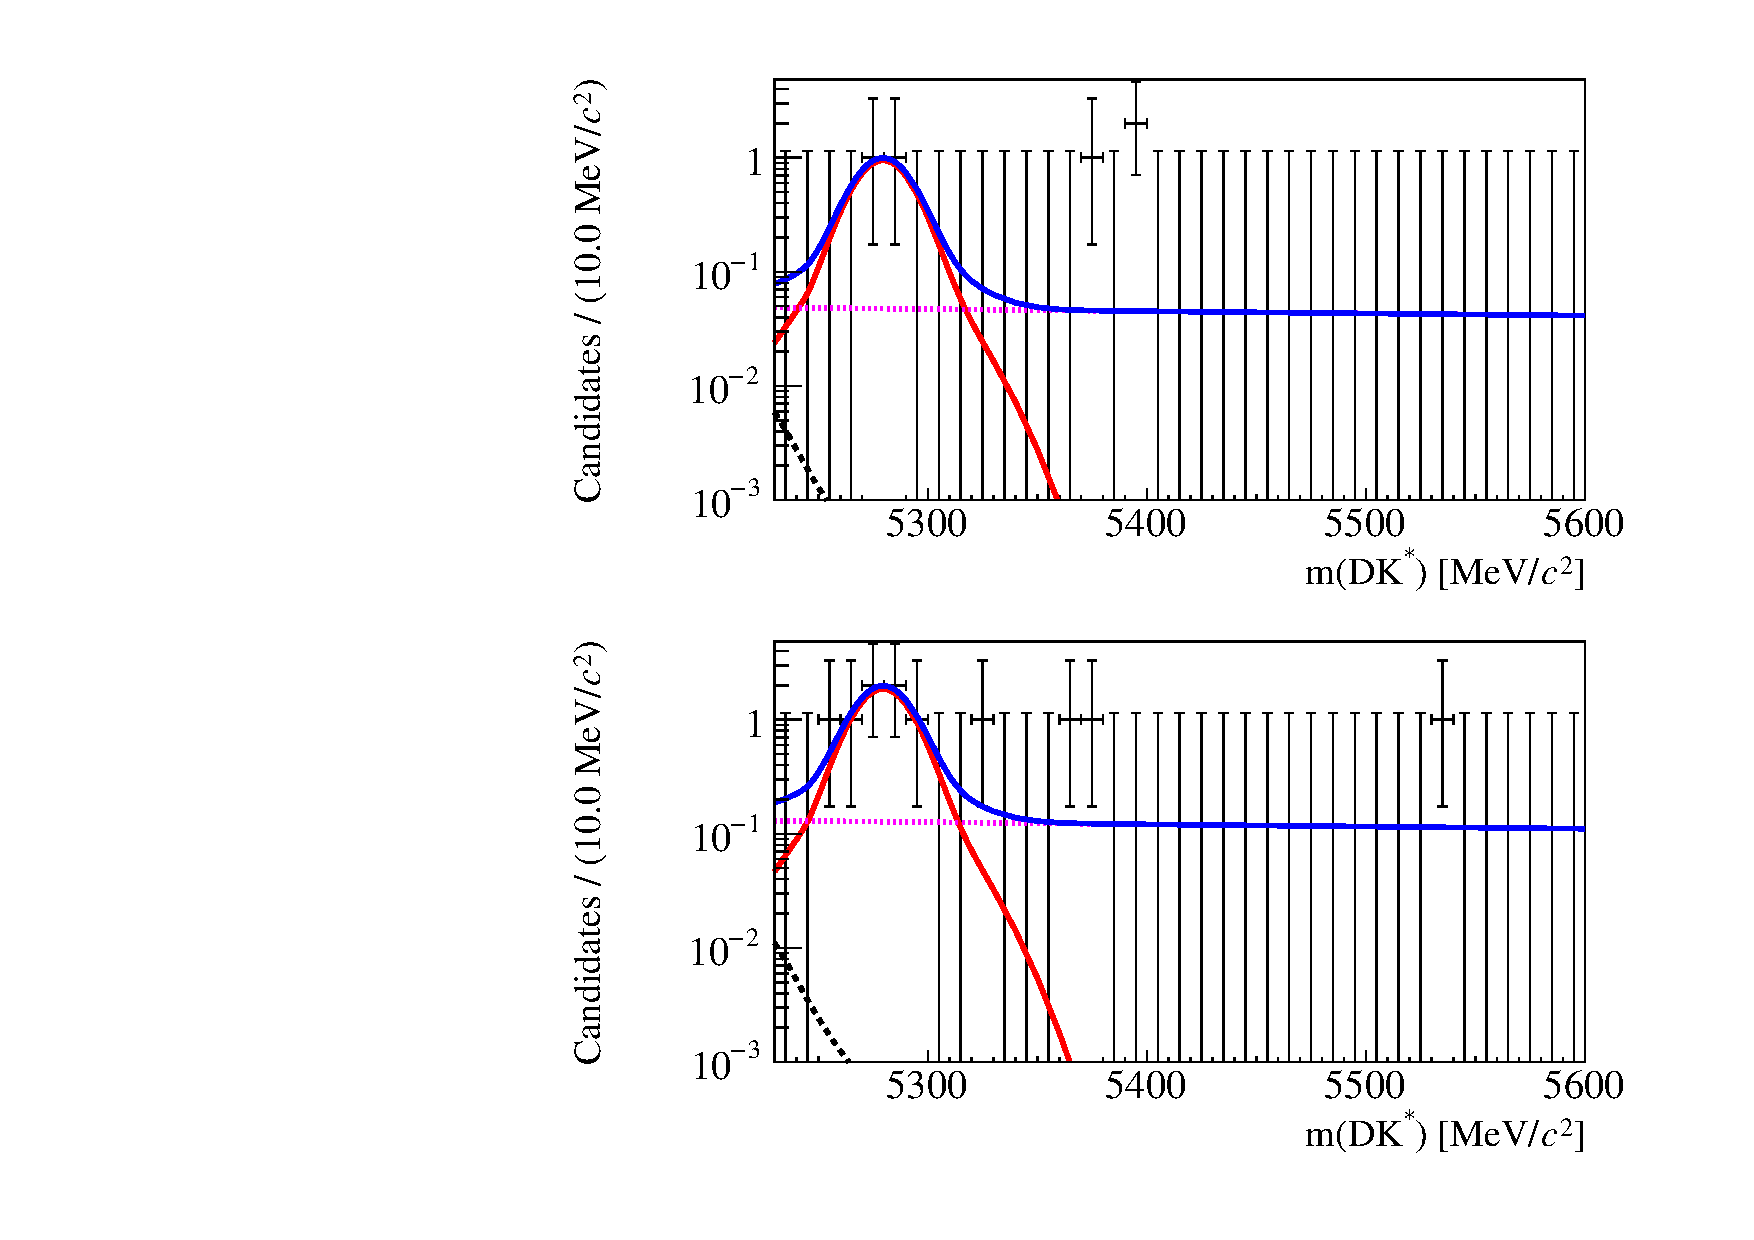
\includegraphics[width=0.3\linewidth]{figures/results/canvaslog_d2pipipipi_LL_run1_log.pdf}}
\hfill
\subfloat[$\pi K\pi\pi$, LL]{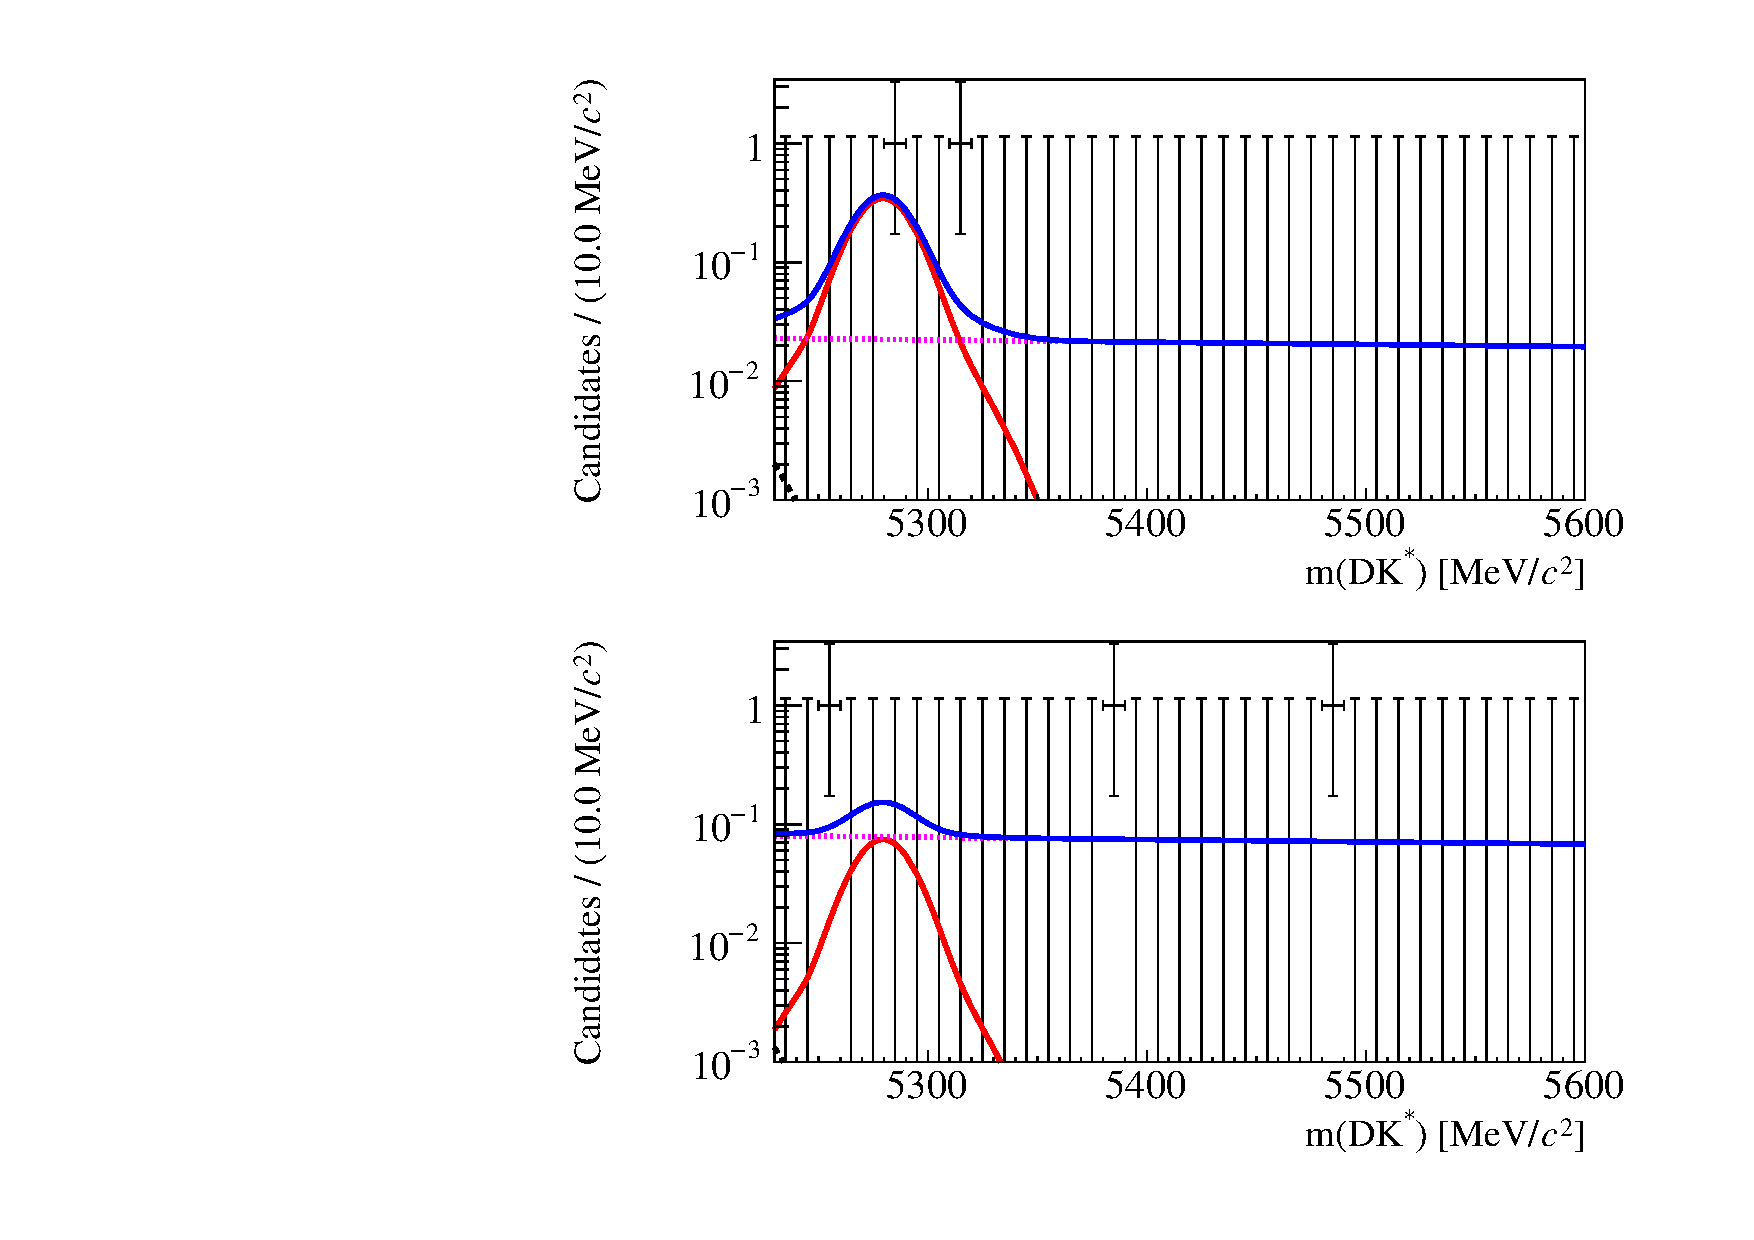
\includegraphics[width=0.3\linewidth]{figures/results/canvaslog_d2pikpipi_LL_run1_log.pdf}}
\hfill
\subfloat[$K\pi\pi\pi$, DD]{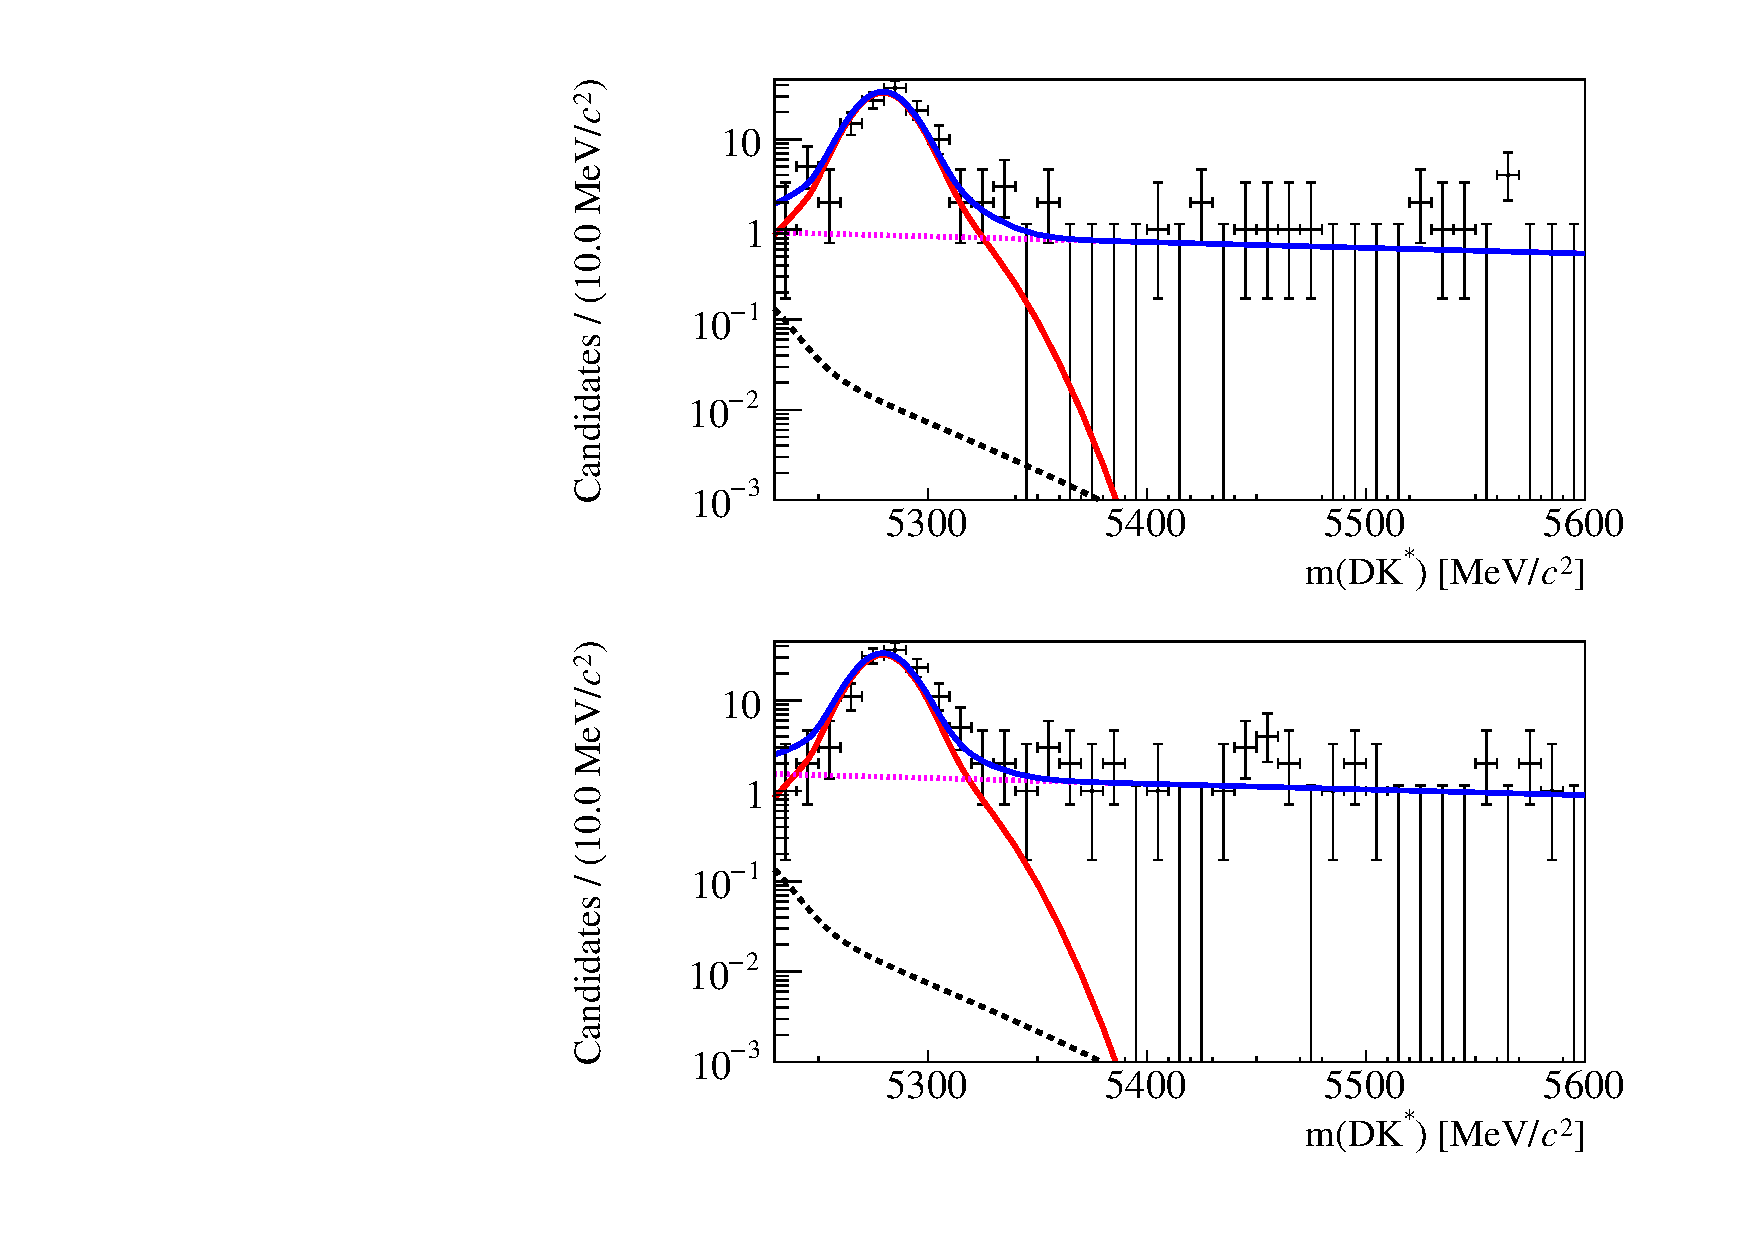
\includegraphics[width=0.3\linewidth]{figures/results/canvaslog_d2kpipipi_DD_run1_log.pdf}}
\hfill
\subfloat[$\pi\pi\pi\pi$, DD]{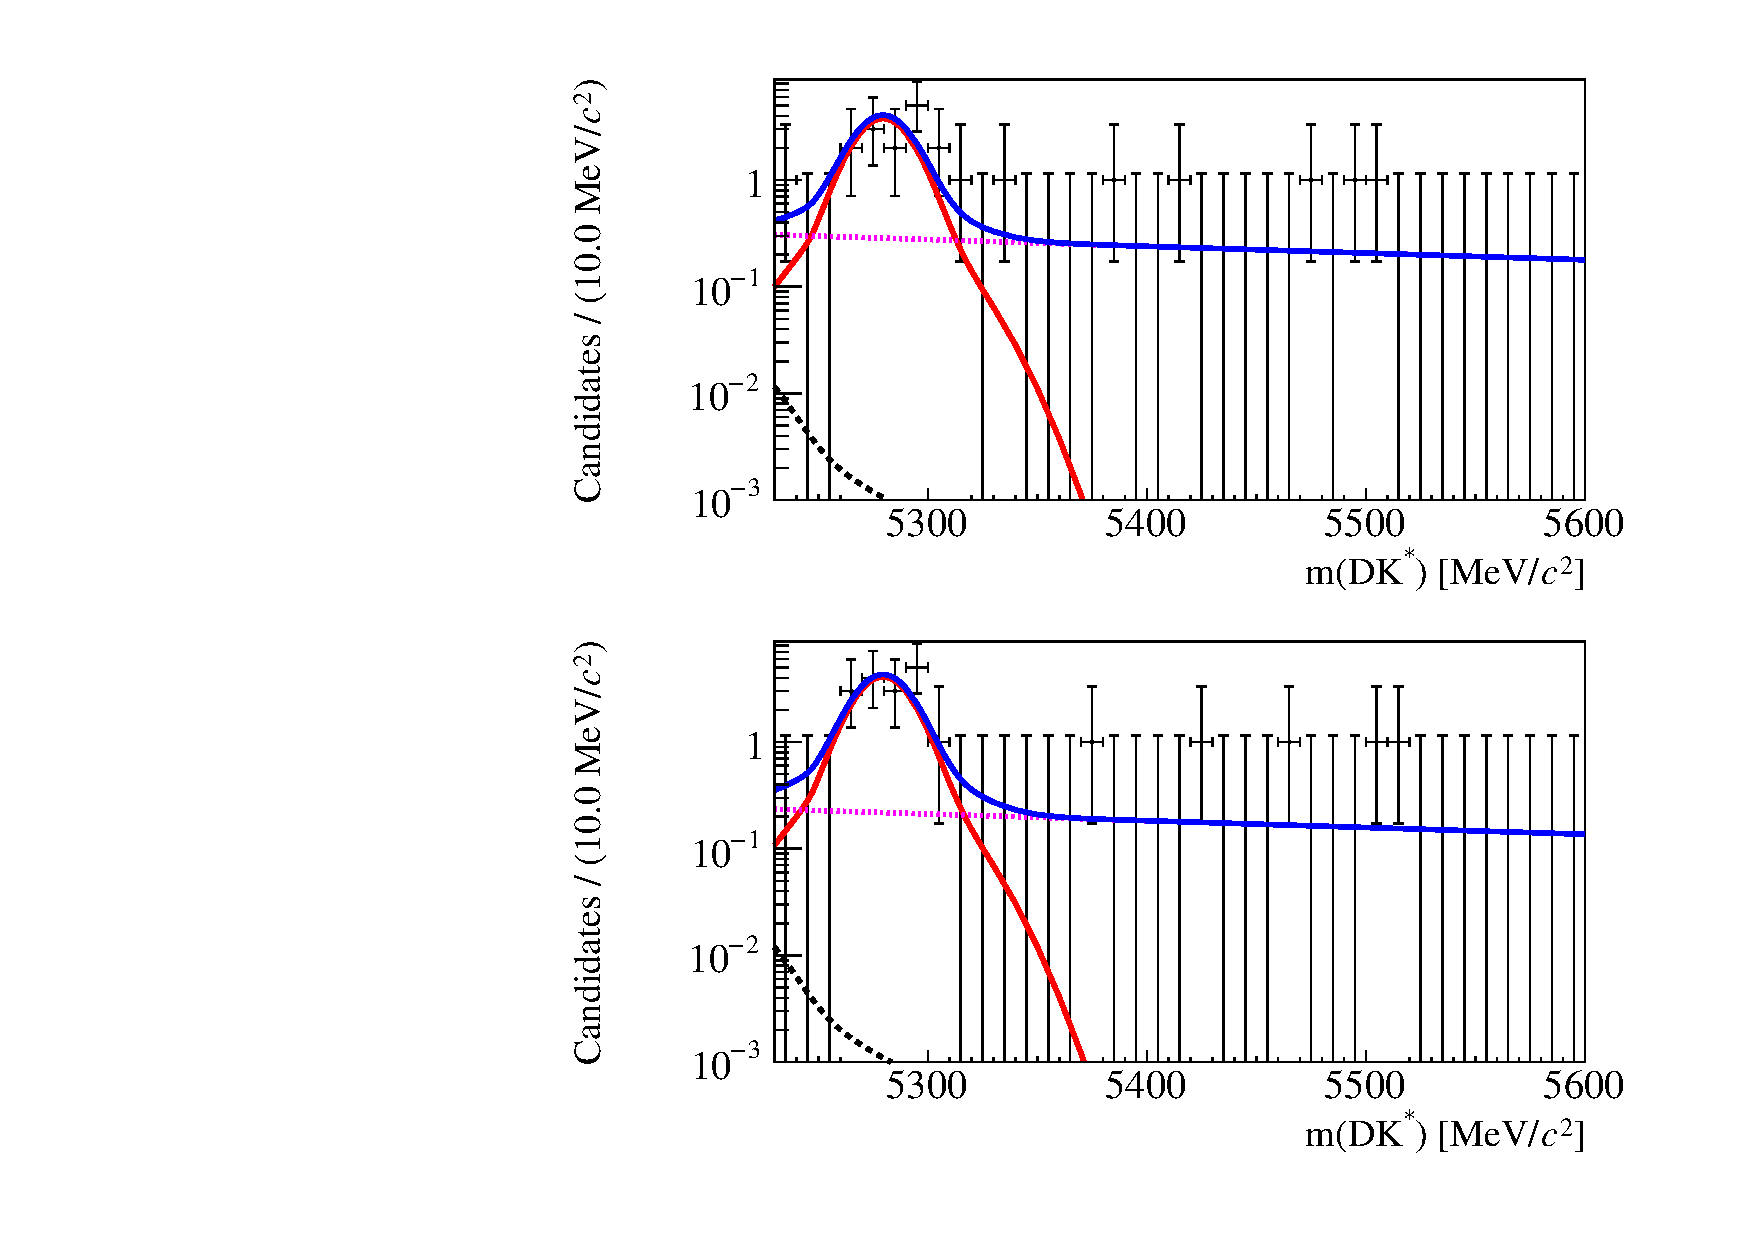
\includegraphics[width=0.3\linewidth]{figures/results/canvaslog_d2pipipipi_DD_run1_log.pdf}}
\hfill
\subfloat[$\pi K\pi\pi$, DD]{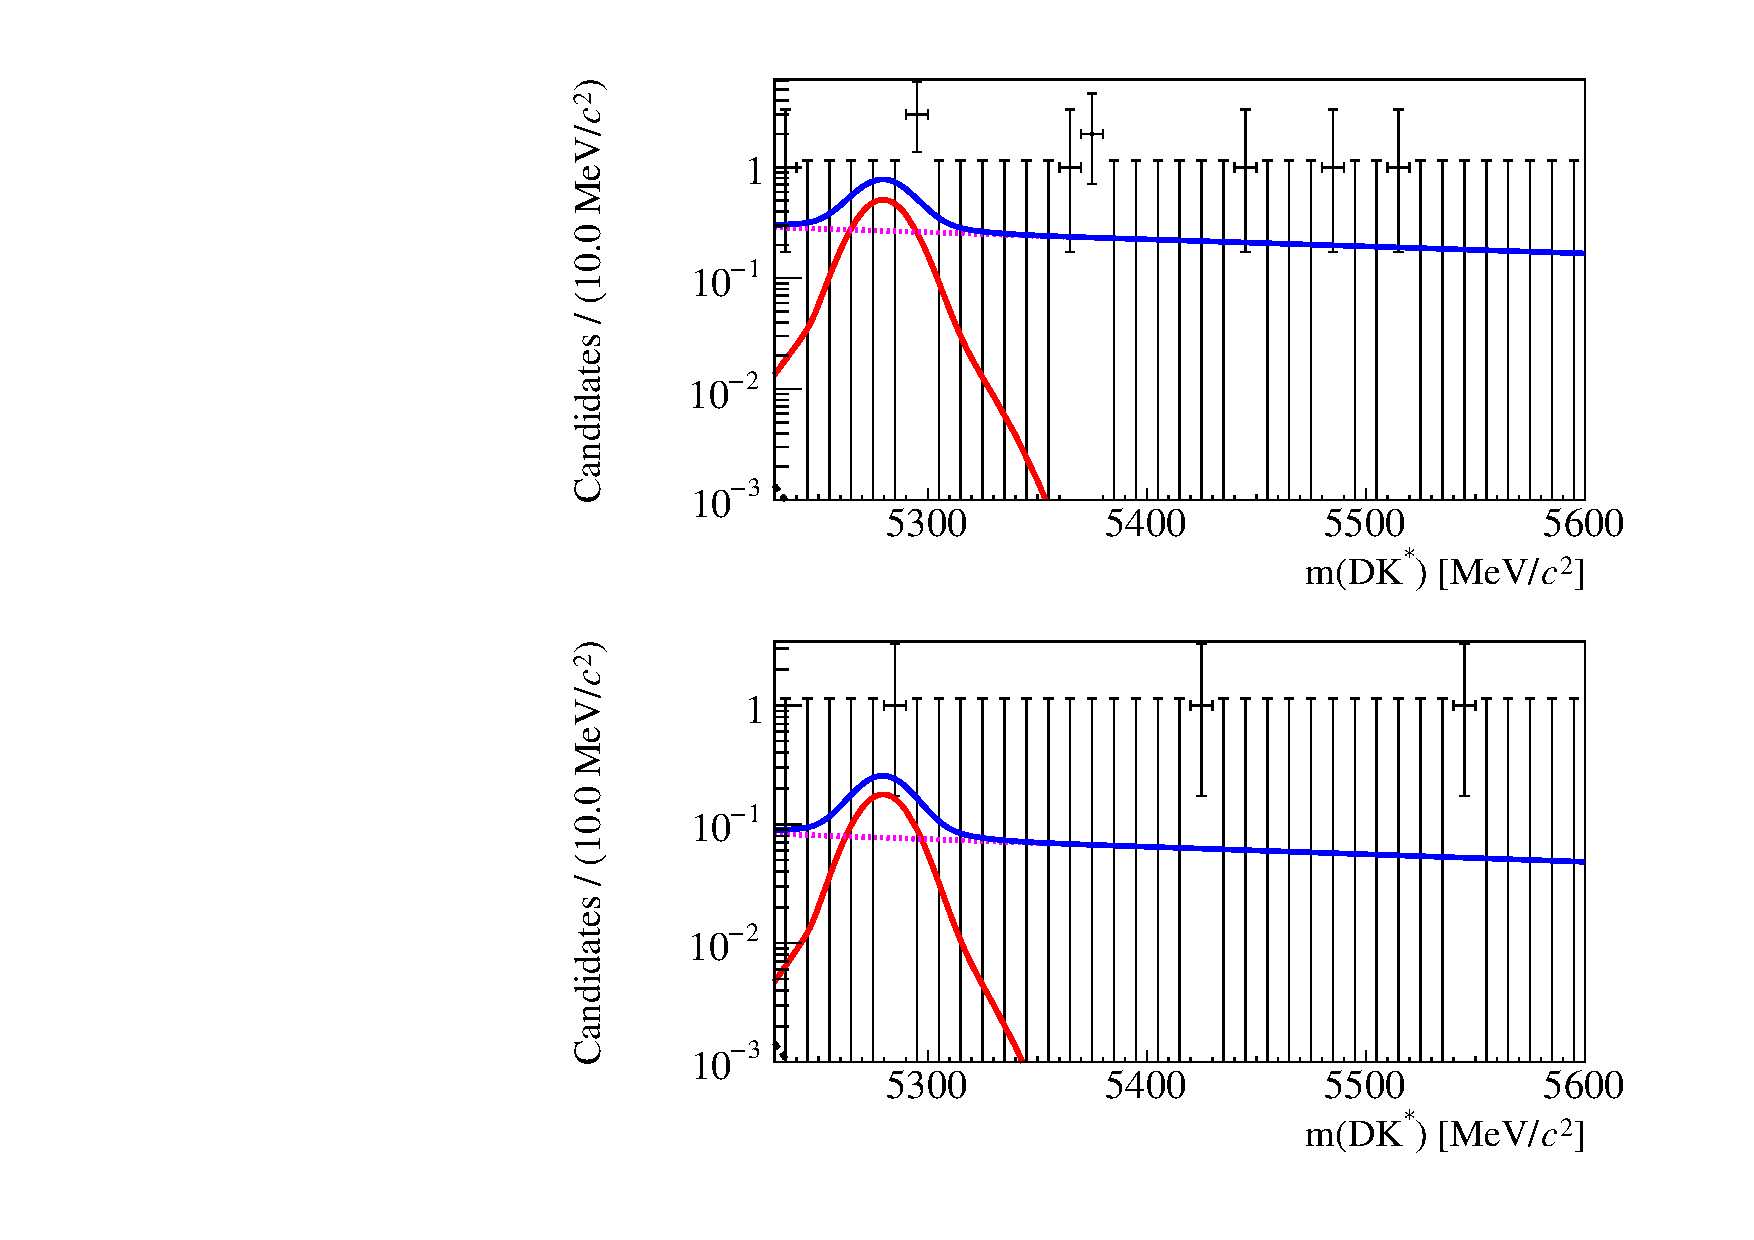
\includegraphics[width=0.3\linewidth]{figures/results/canvaslog_d2pikpipi_DD_run1_log.pdf}}
\caption{Results of the simultaneous fit for Run 1 data for 4-body modes. In each pair the top plot is for \Bp decays and the bottom plot is for \Bm decays.}
\label{datafit4bodyRun1}
\end{sidewaysfigure}

\begin{sidewaysfigure}[h]
\centering
\subfloat[$K\pi$, LL]{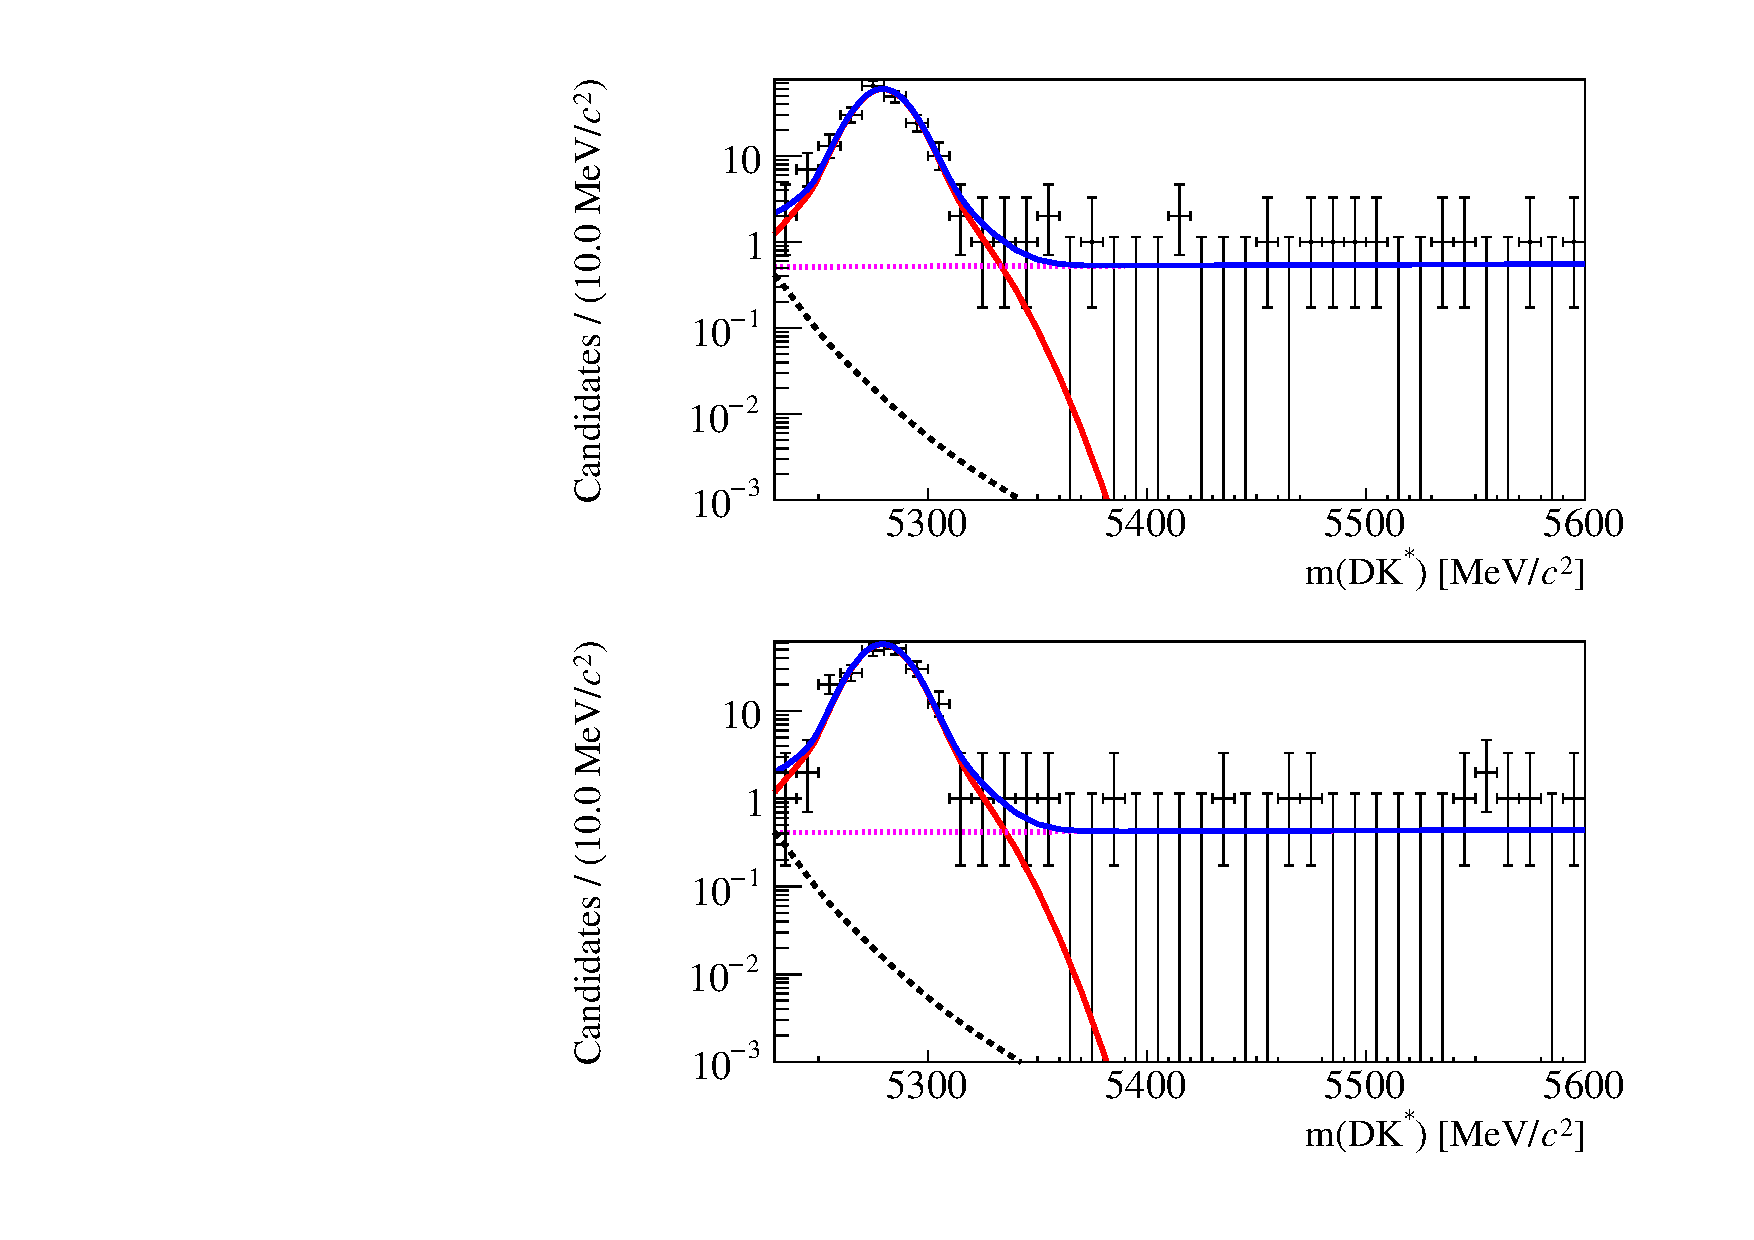
\includegraphics[width=0.25\linewidth]{figures/results/canvaslog_d2kpi_LL_run2_log.pdf}}
\hfill
\subfloat[$KK$, LL]{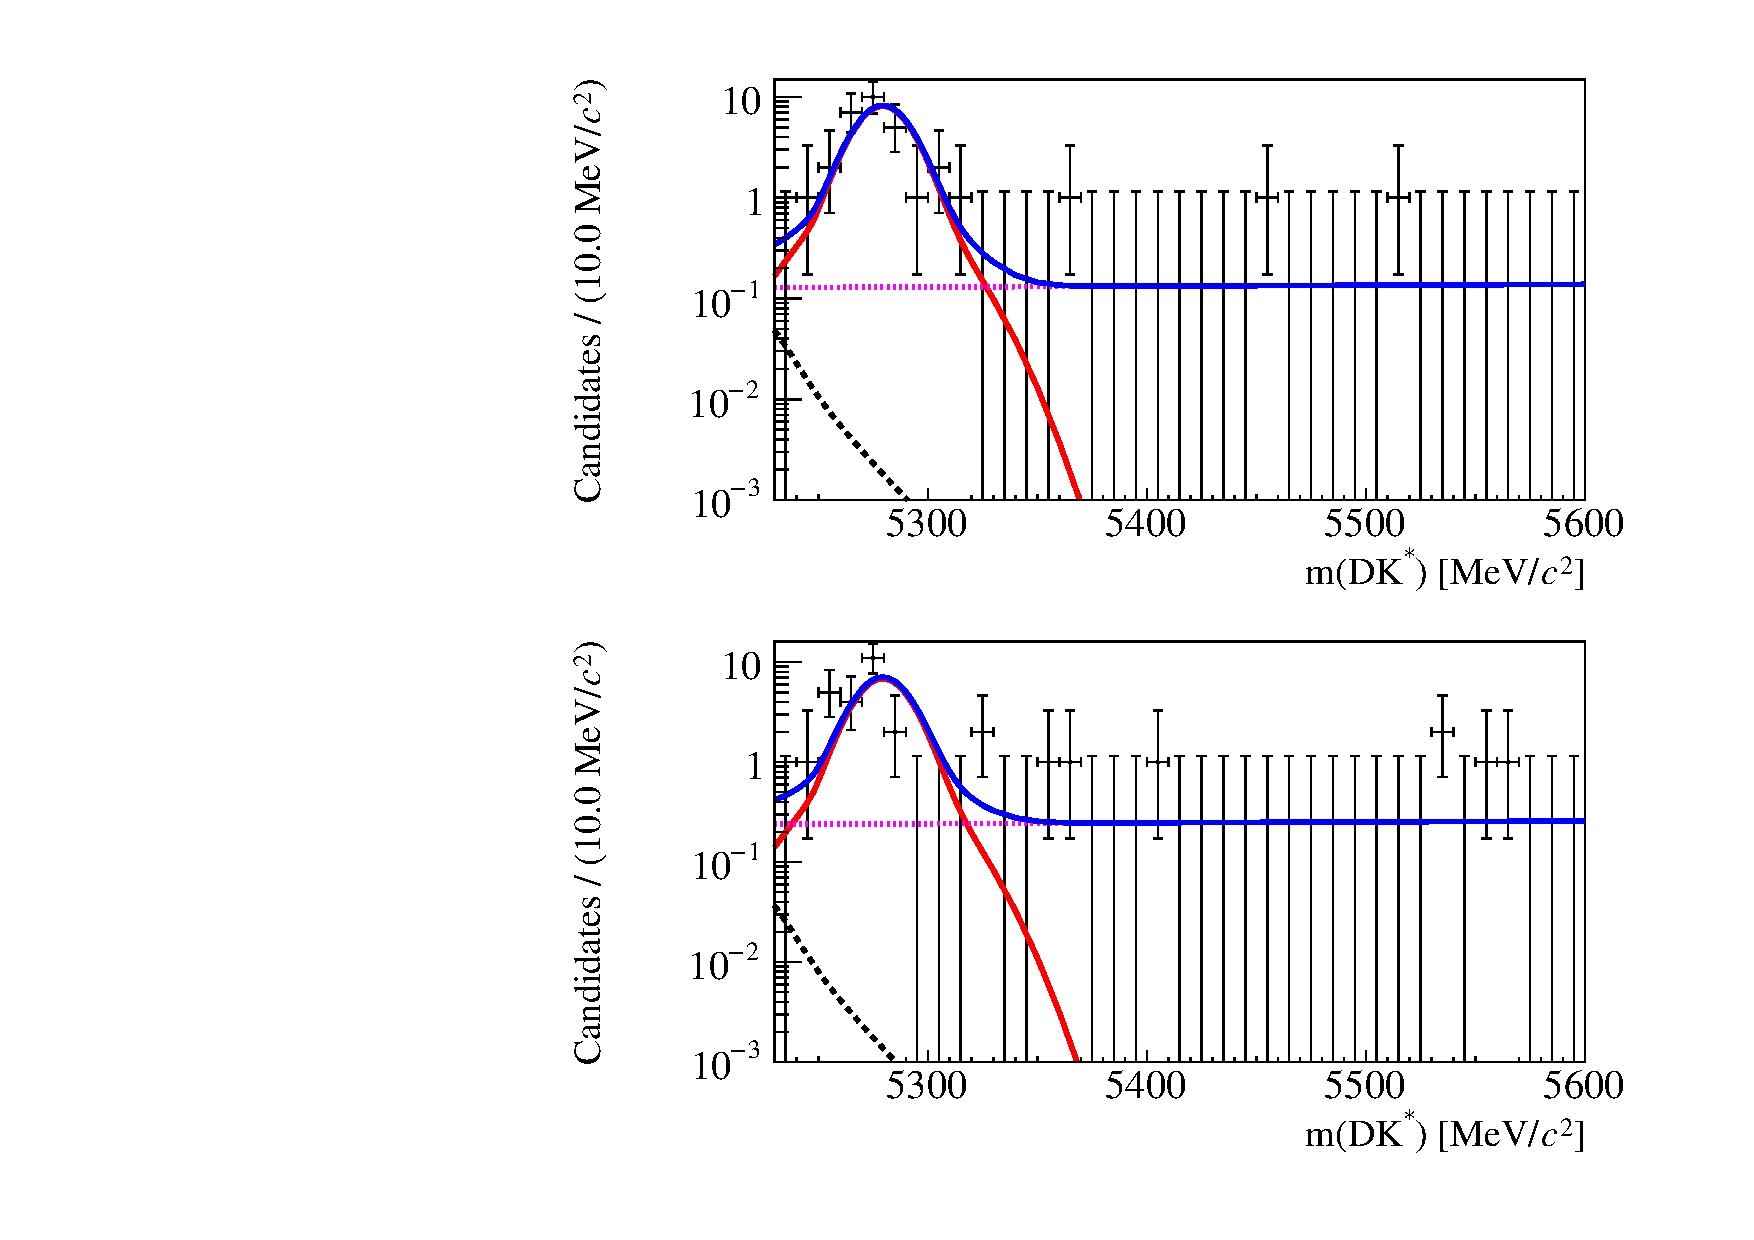
\includegraphics[width=0.25\linewidth]{figures/results/canvaslog_d2kk_LL_run2_log.pdf}}
\hfill
\subfloat[$\pi\pi$, LL]{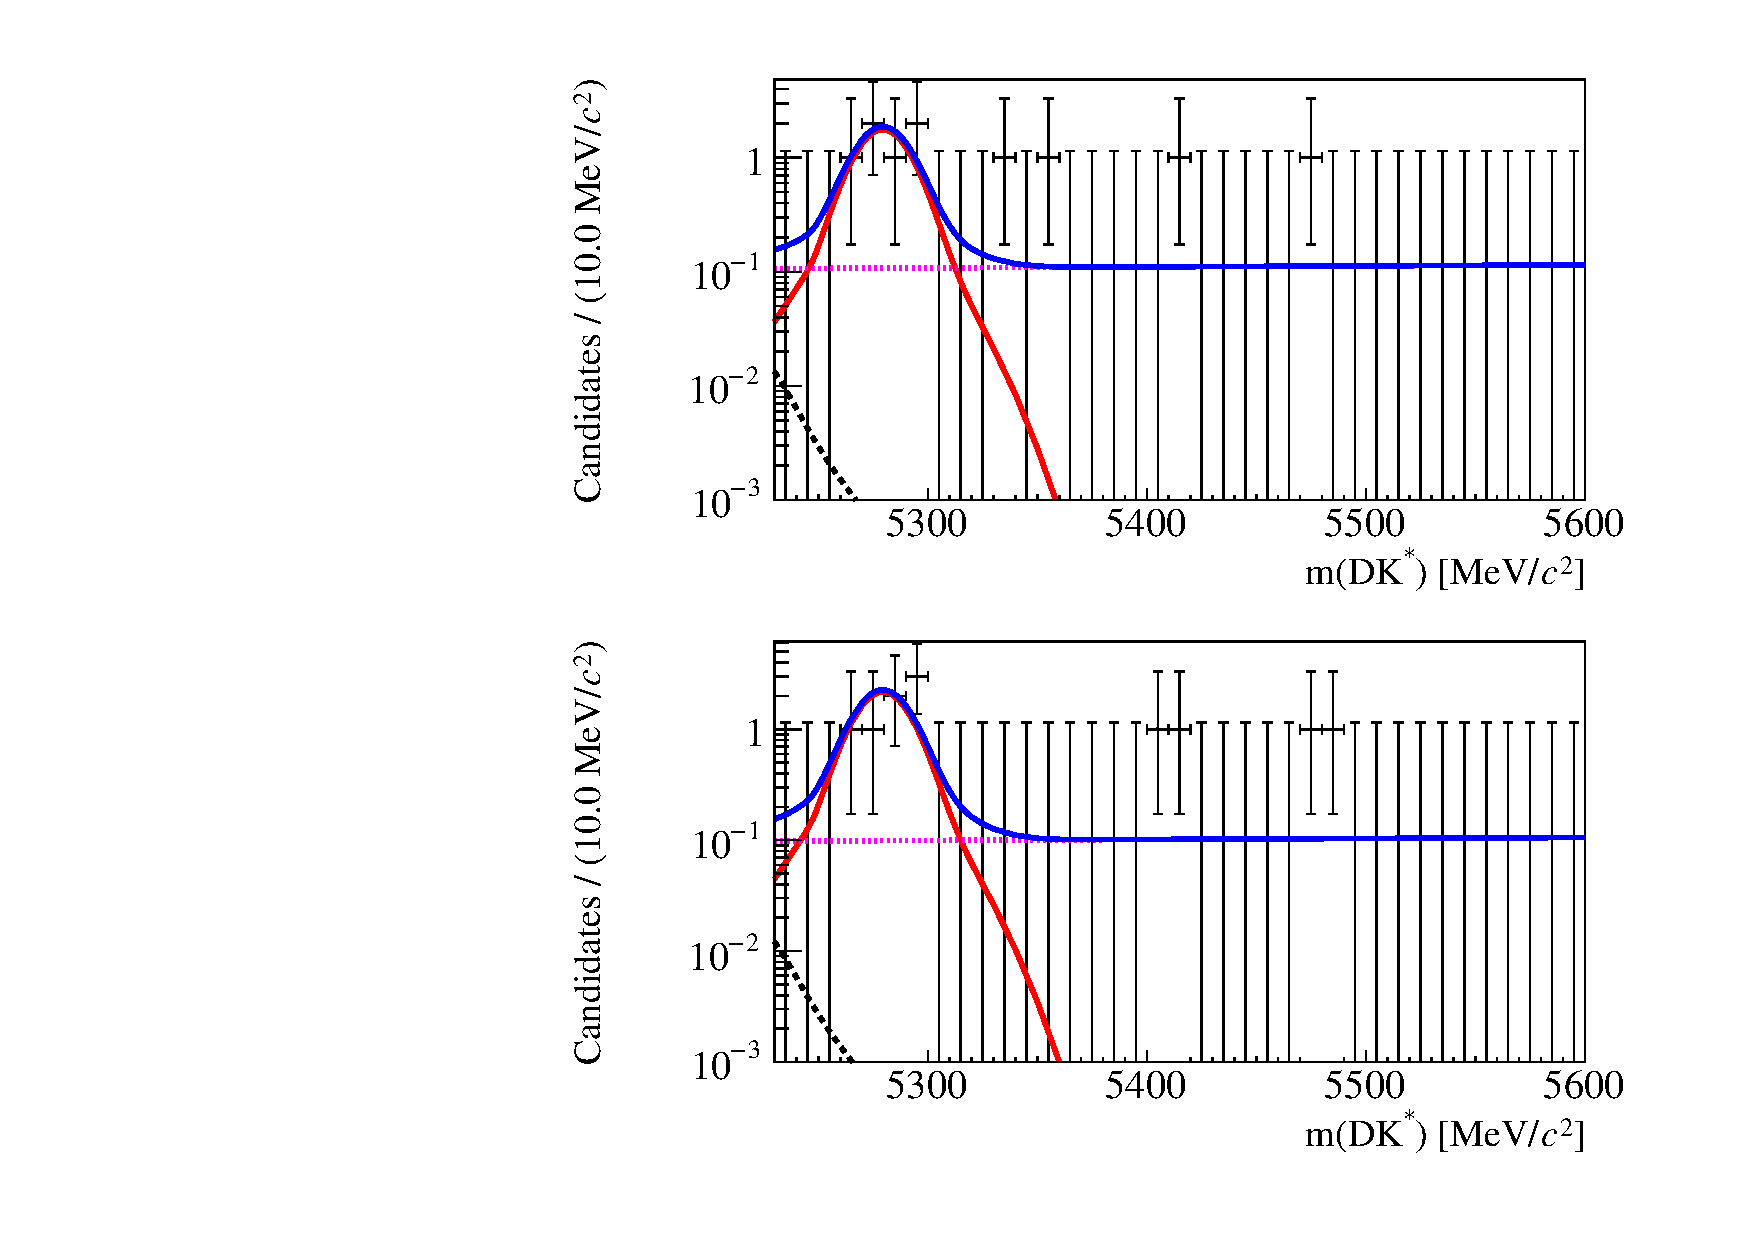
\includegraphics[width=0.25\linewidth]{figures/results/canvaslog_d2pipi_LL_run2_log.pdf}}
\hfill
\subfloat[$\pi K$, LL]{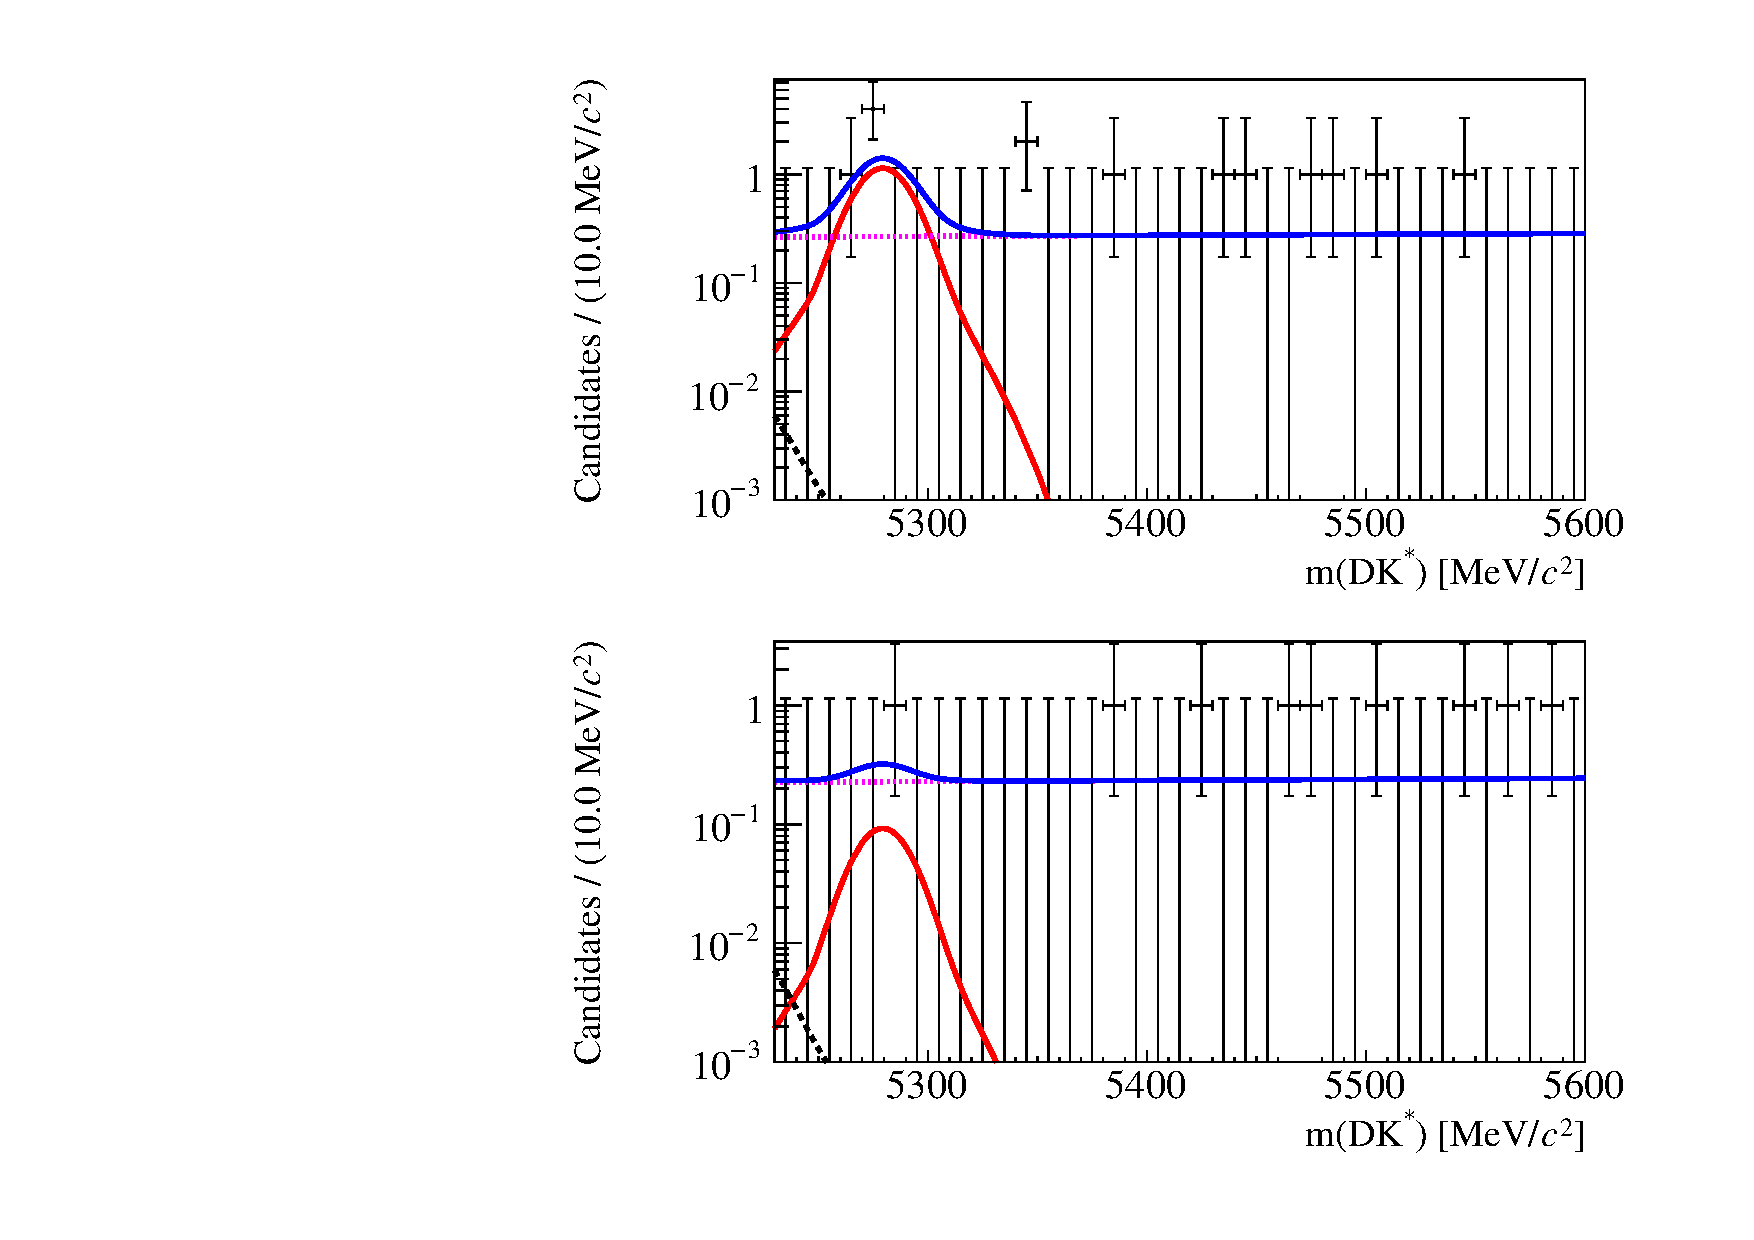
\includegraphics[width=0.25\linewidth]{figures/results/canvaslog_d2pik_LL_run2_log.pdf}}
\hfill
\subfloat[$K\pi$, DD]{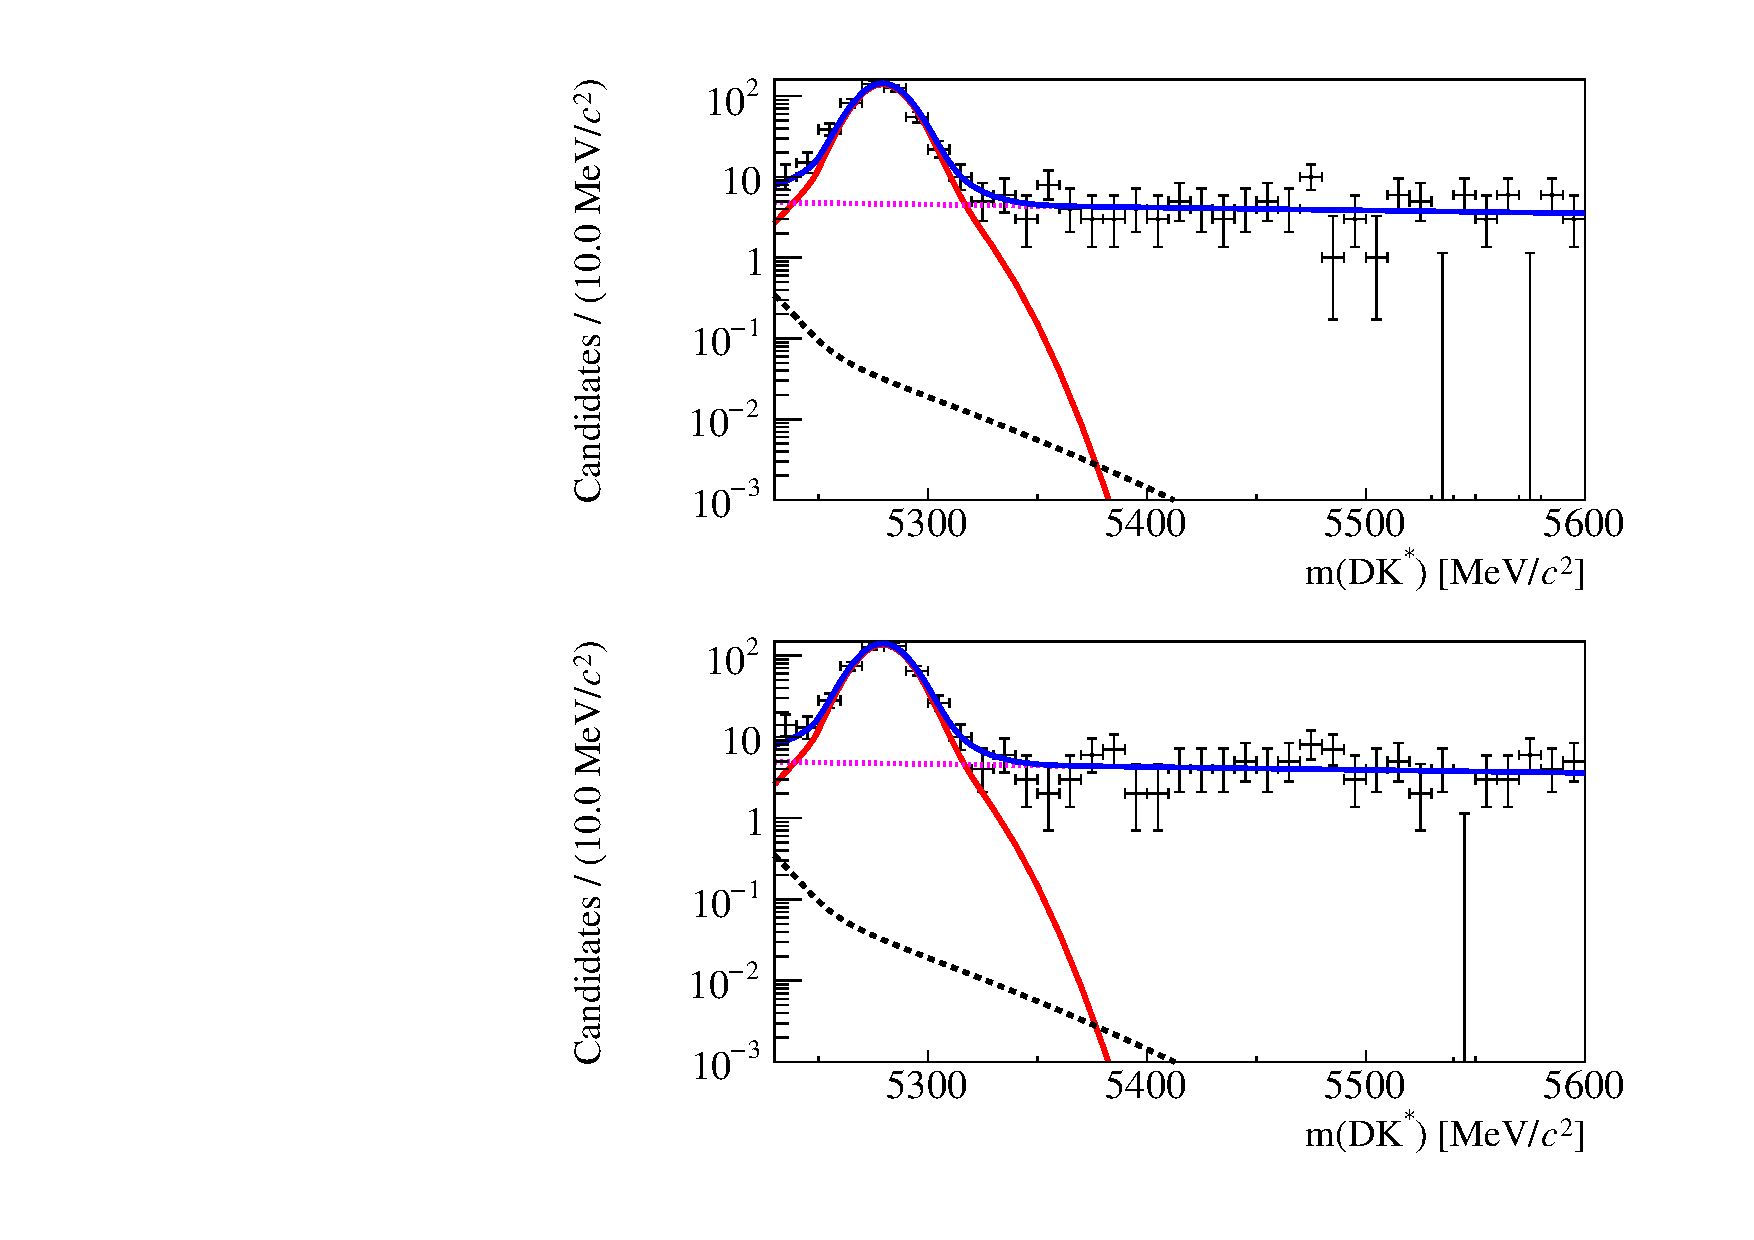
\includegraphics[width=0.25\linewidth]{figures/results/canvaslog_d2kpi_DD_run2_log.pdf}}
\hfill
\subfloat[$KK$, DD]{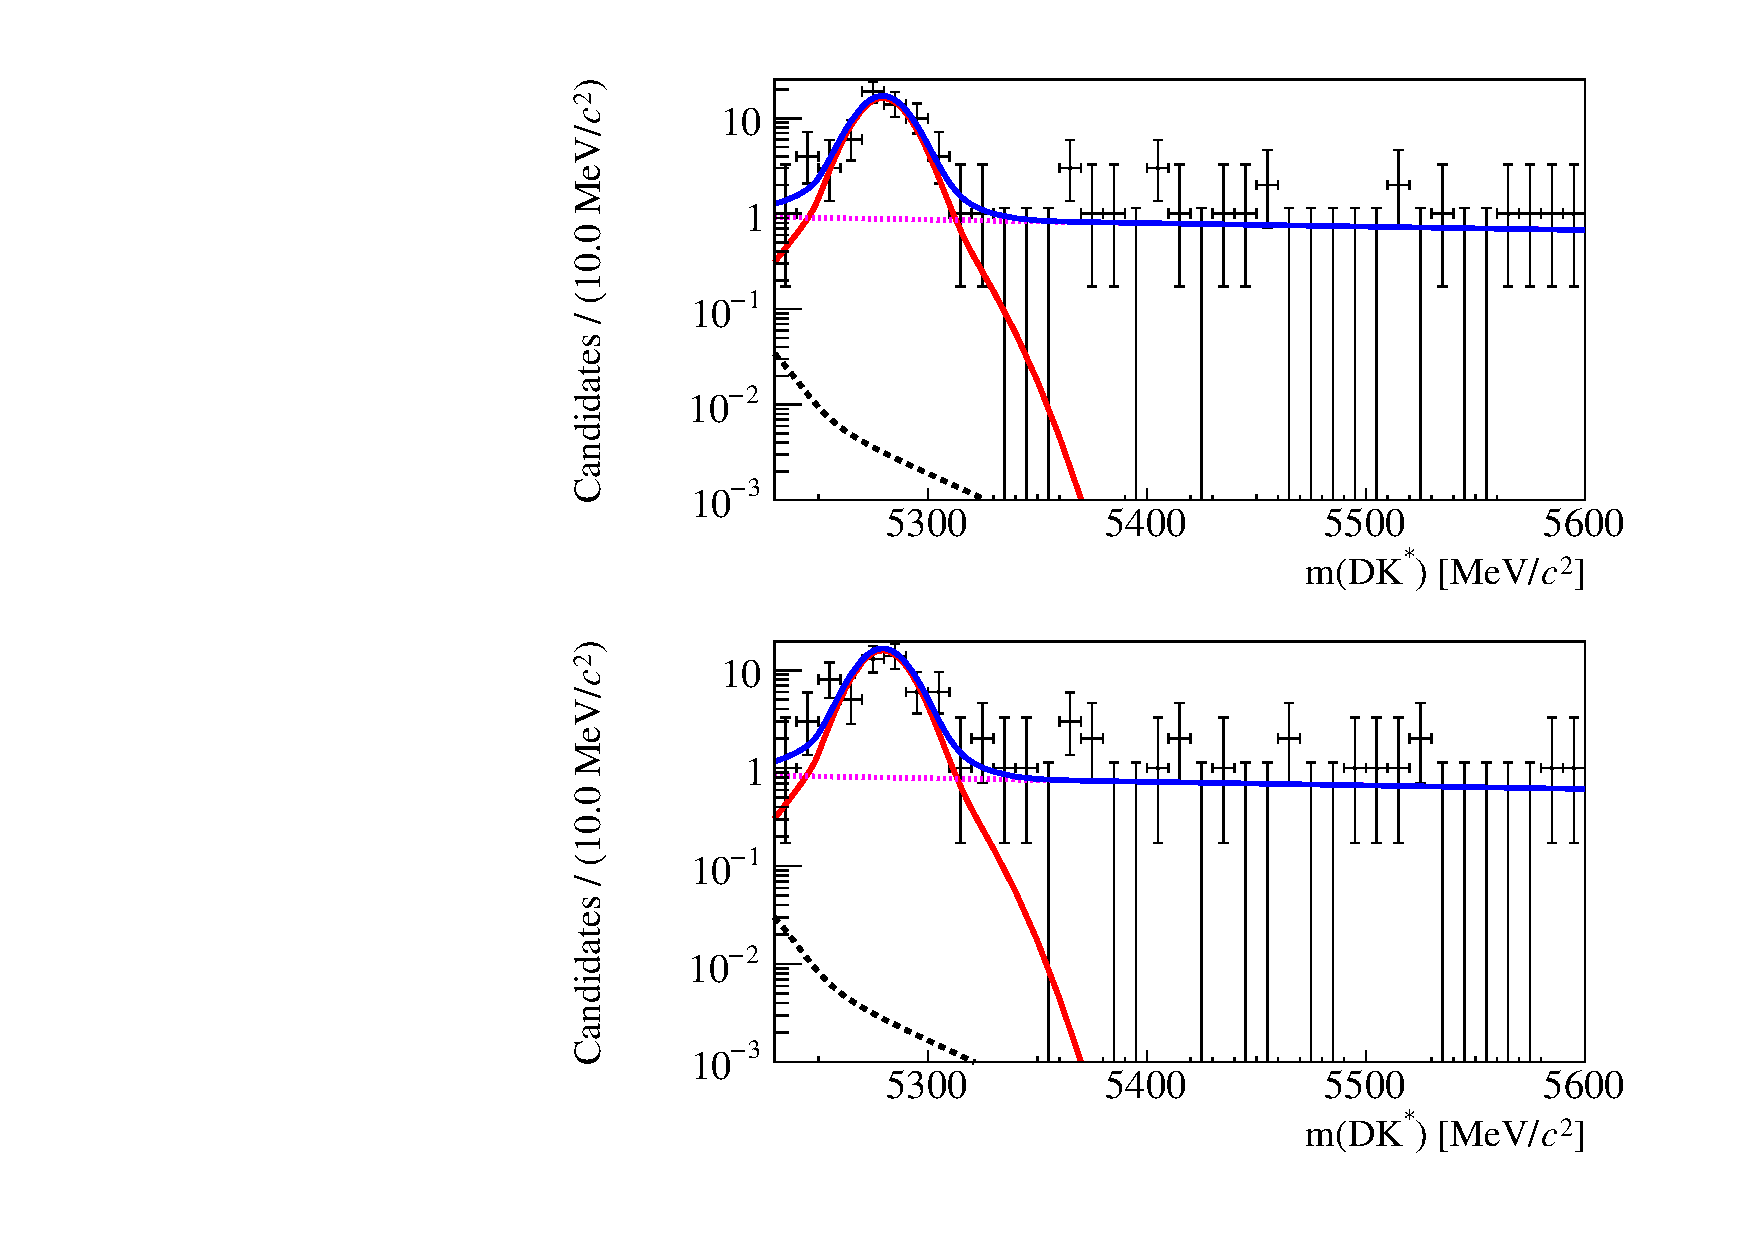
\includegraphics[width=0.25\linewidth]{figures/results/canvaslog_d2kk_DD_run2_log.pdf}}
\hfill
\subfloat[$\pi\pi$, DD]{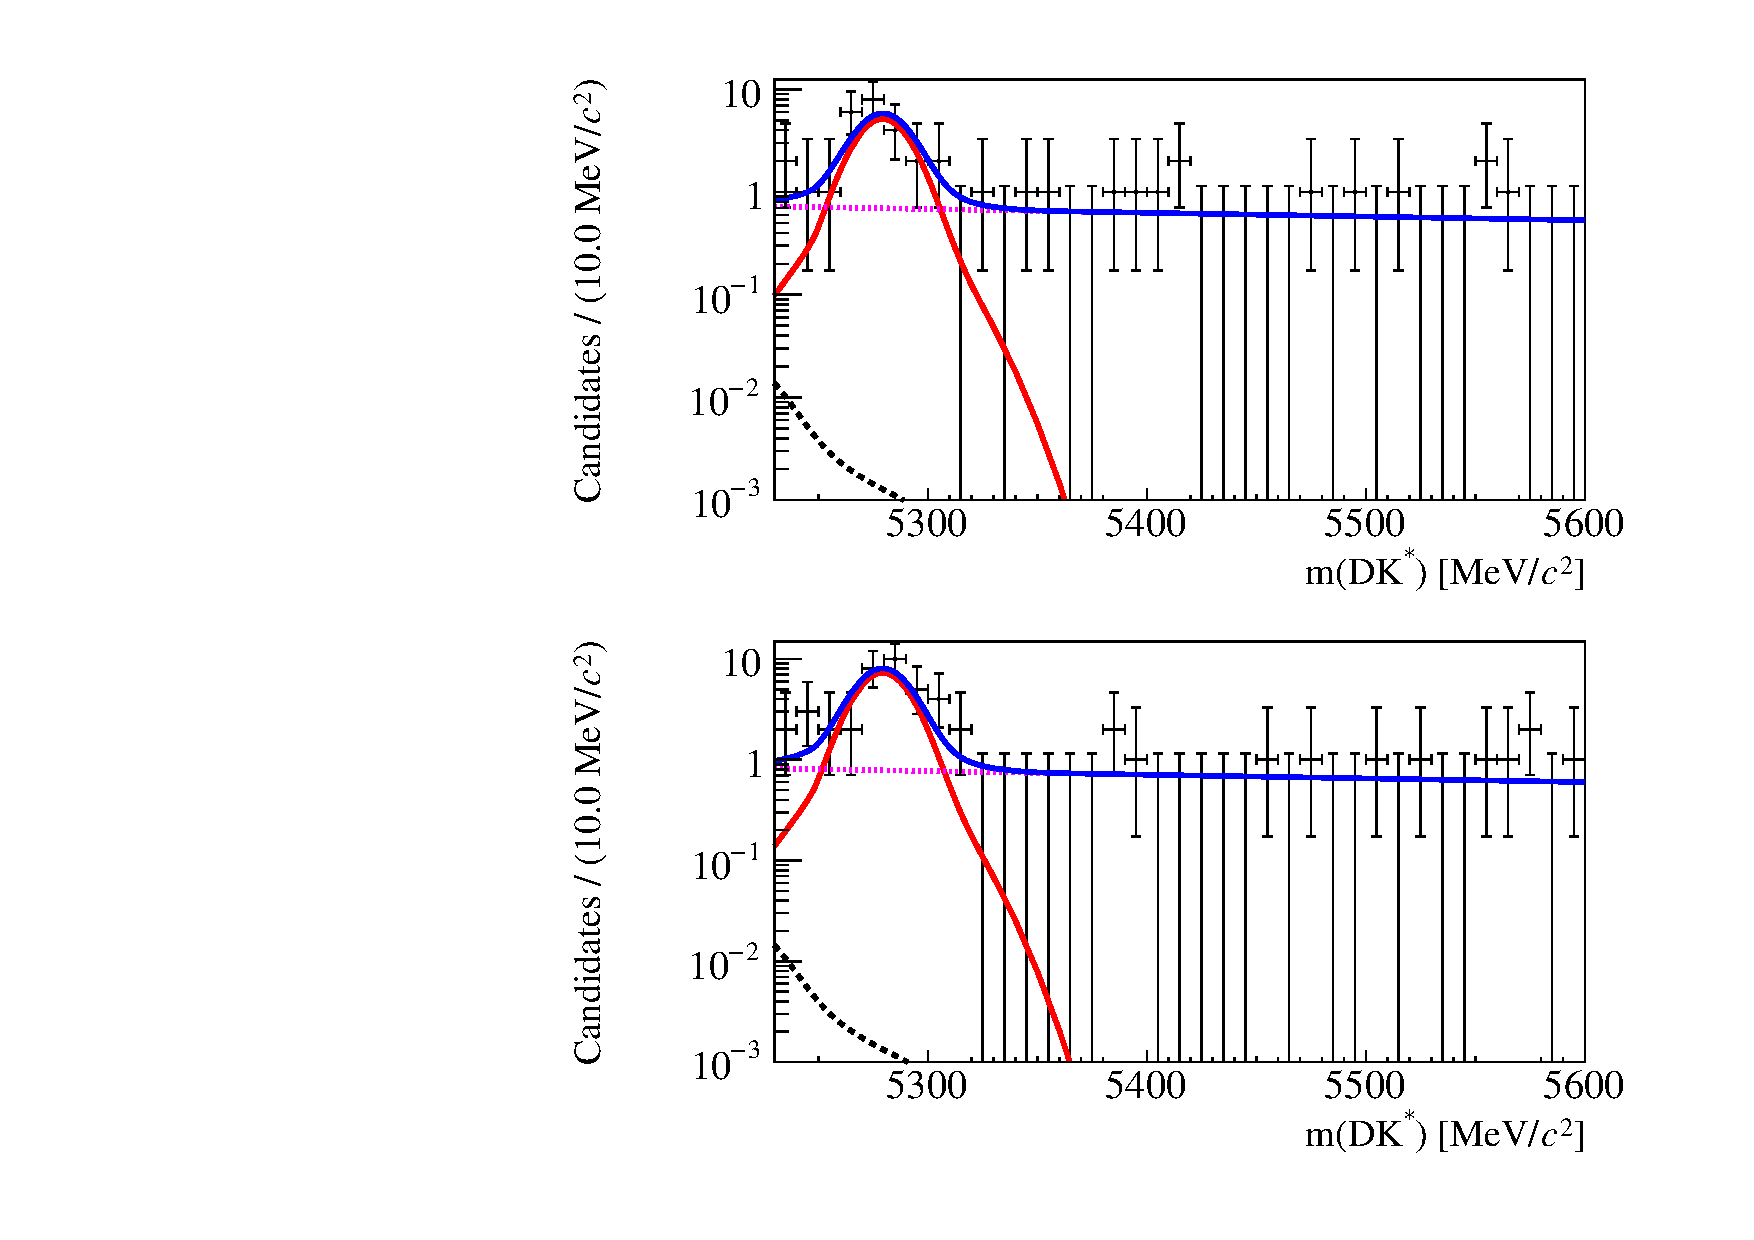
\includegraphics[width=0.25\linewidth]{figures/results/canvaslog_d2pipi_DD_run2_log.pdf}}
\hfill
\subfloat[$\pi K$, DD]{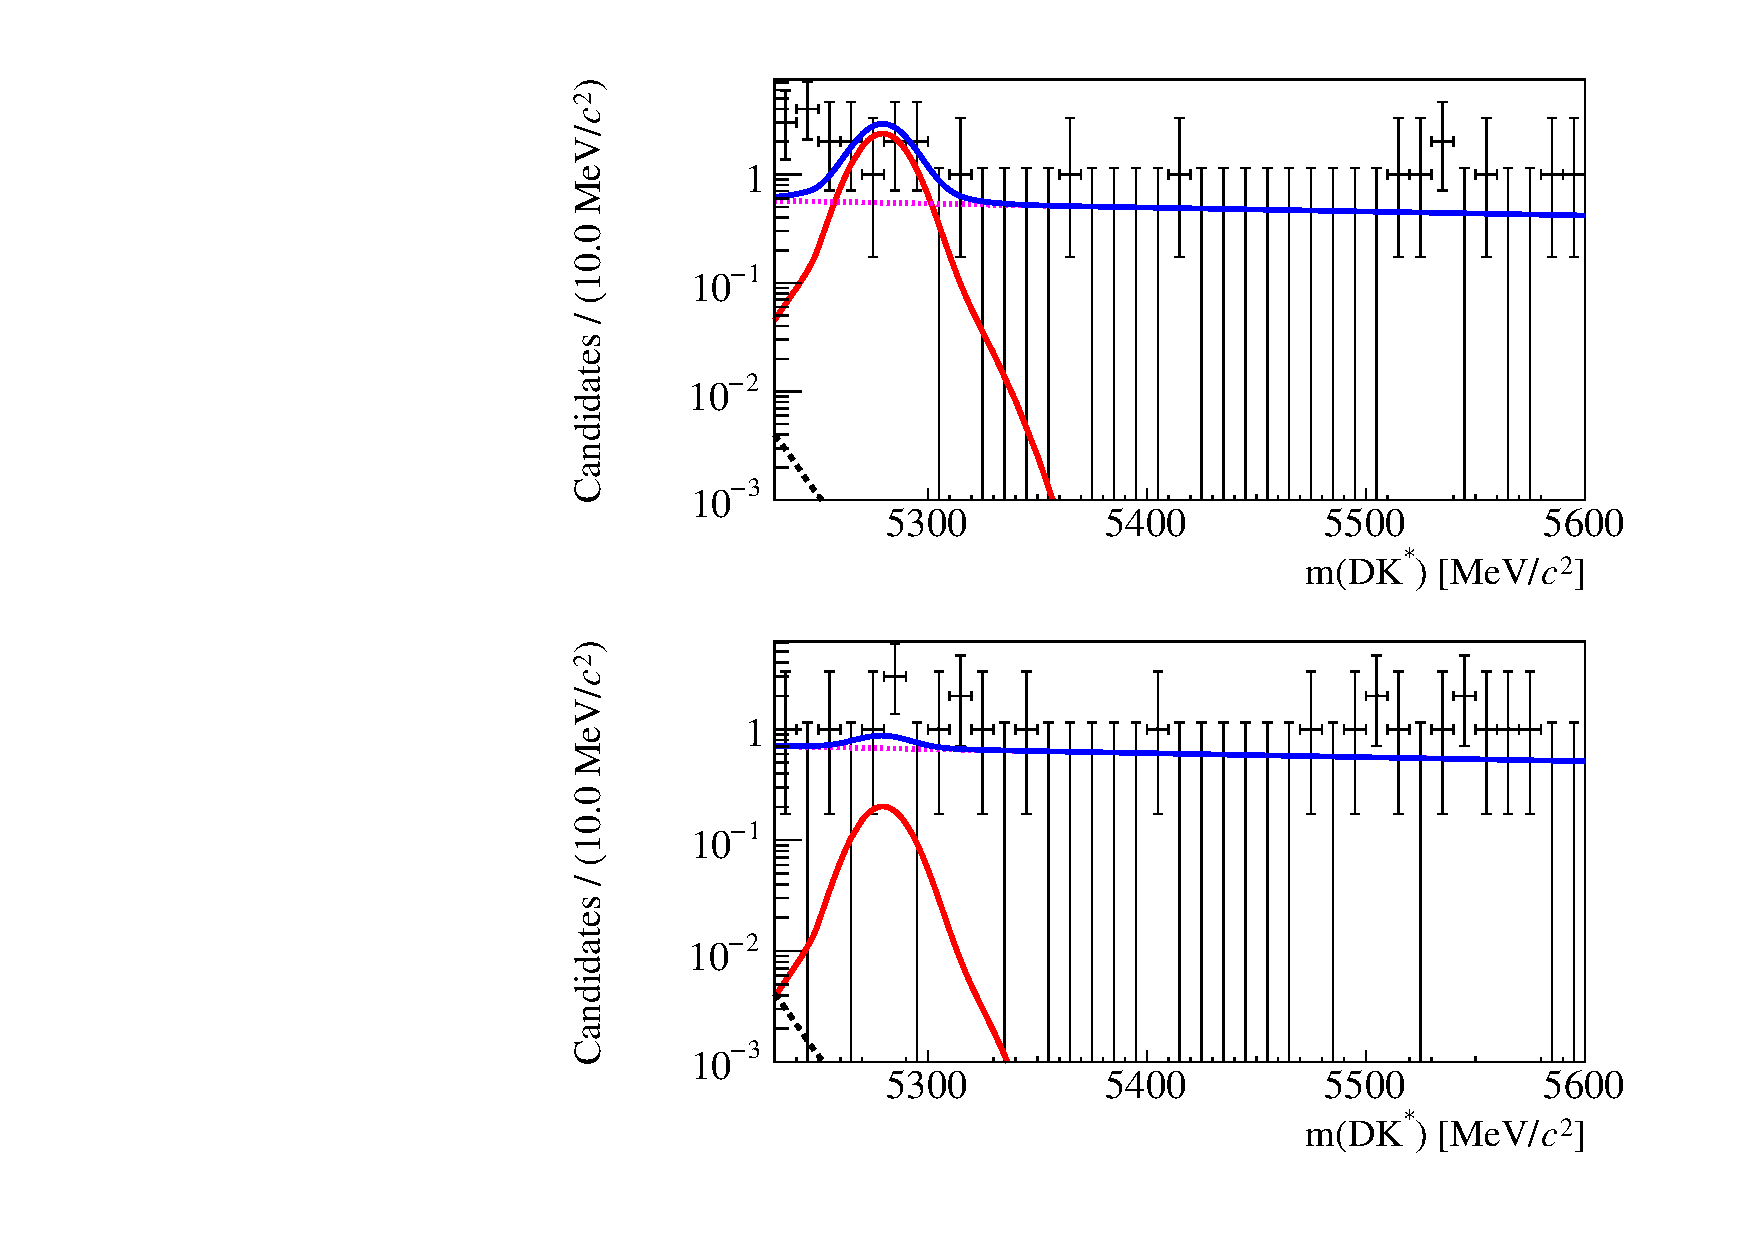
\includegraphics[width=0.25\linewidth]{figures/results/canvaslog_d2pik_DD_run2_log.pdf}}
\caption{Results of the simultaneous fit for Run 1 data for 2-body modes. In each pair the top plot is for \Bp decays and the bottom plot is for \Bm decays.}
\label{datafit2bodyRun2}
\end{sidewaysfigure}

\begin{sidewaysfigure}[h]
\centering
\subfloat[$K\pi\pi\pi$, LL]{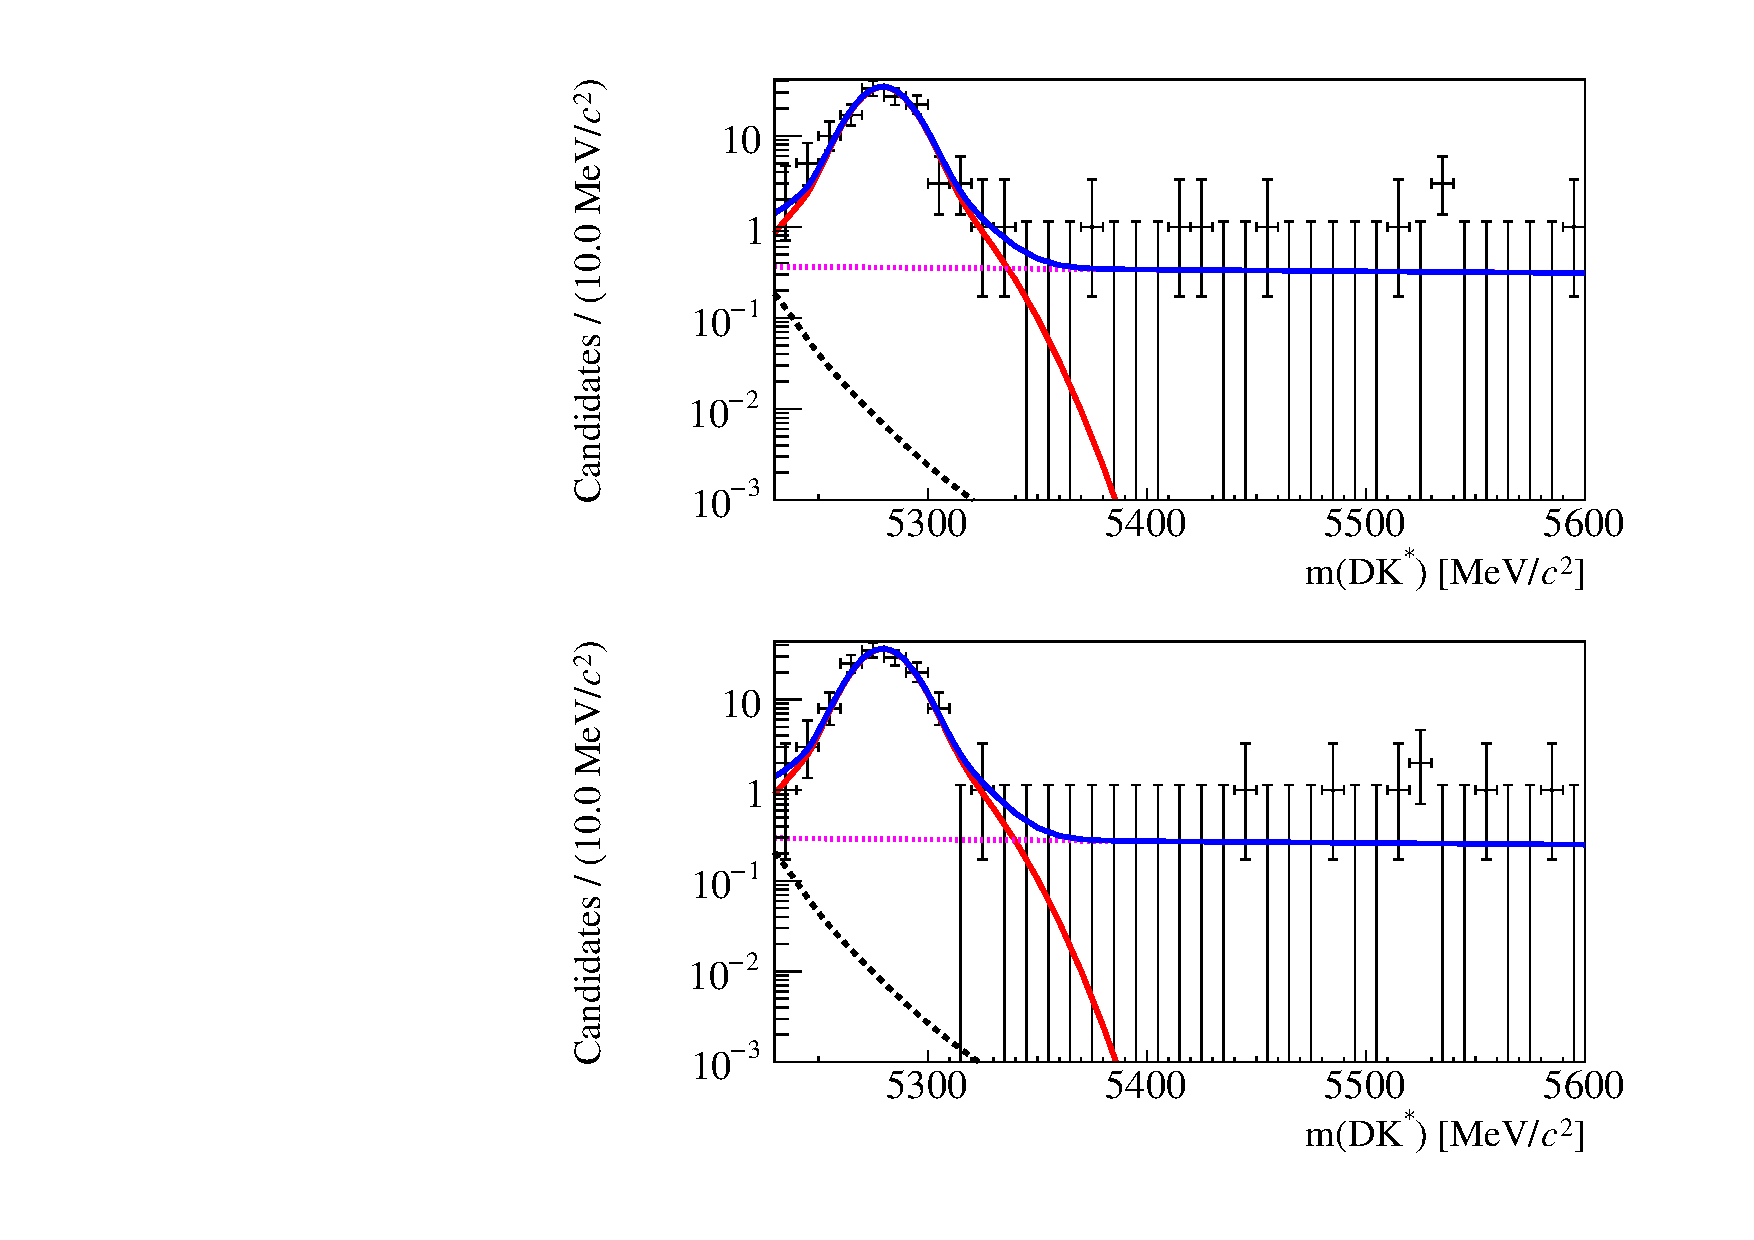
\includegraphics[width=0.3\linewidth]{figures/results/canvaslog_d2kpipipi_LL_run2_log.pdf}}
\hfill
\subfloat[$\pi\pi\pi\pi$, LL]{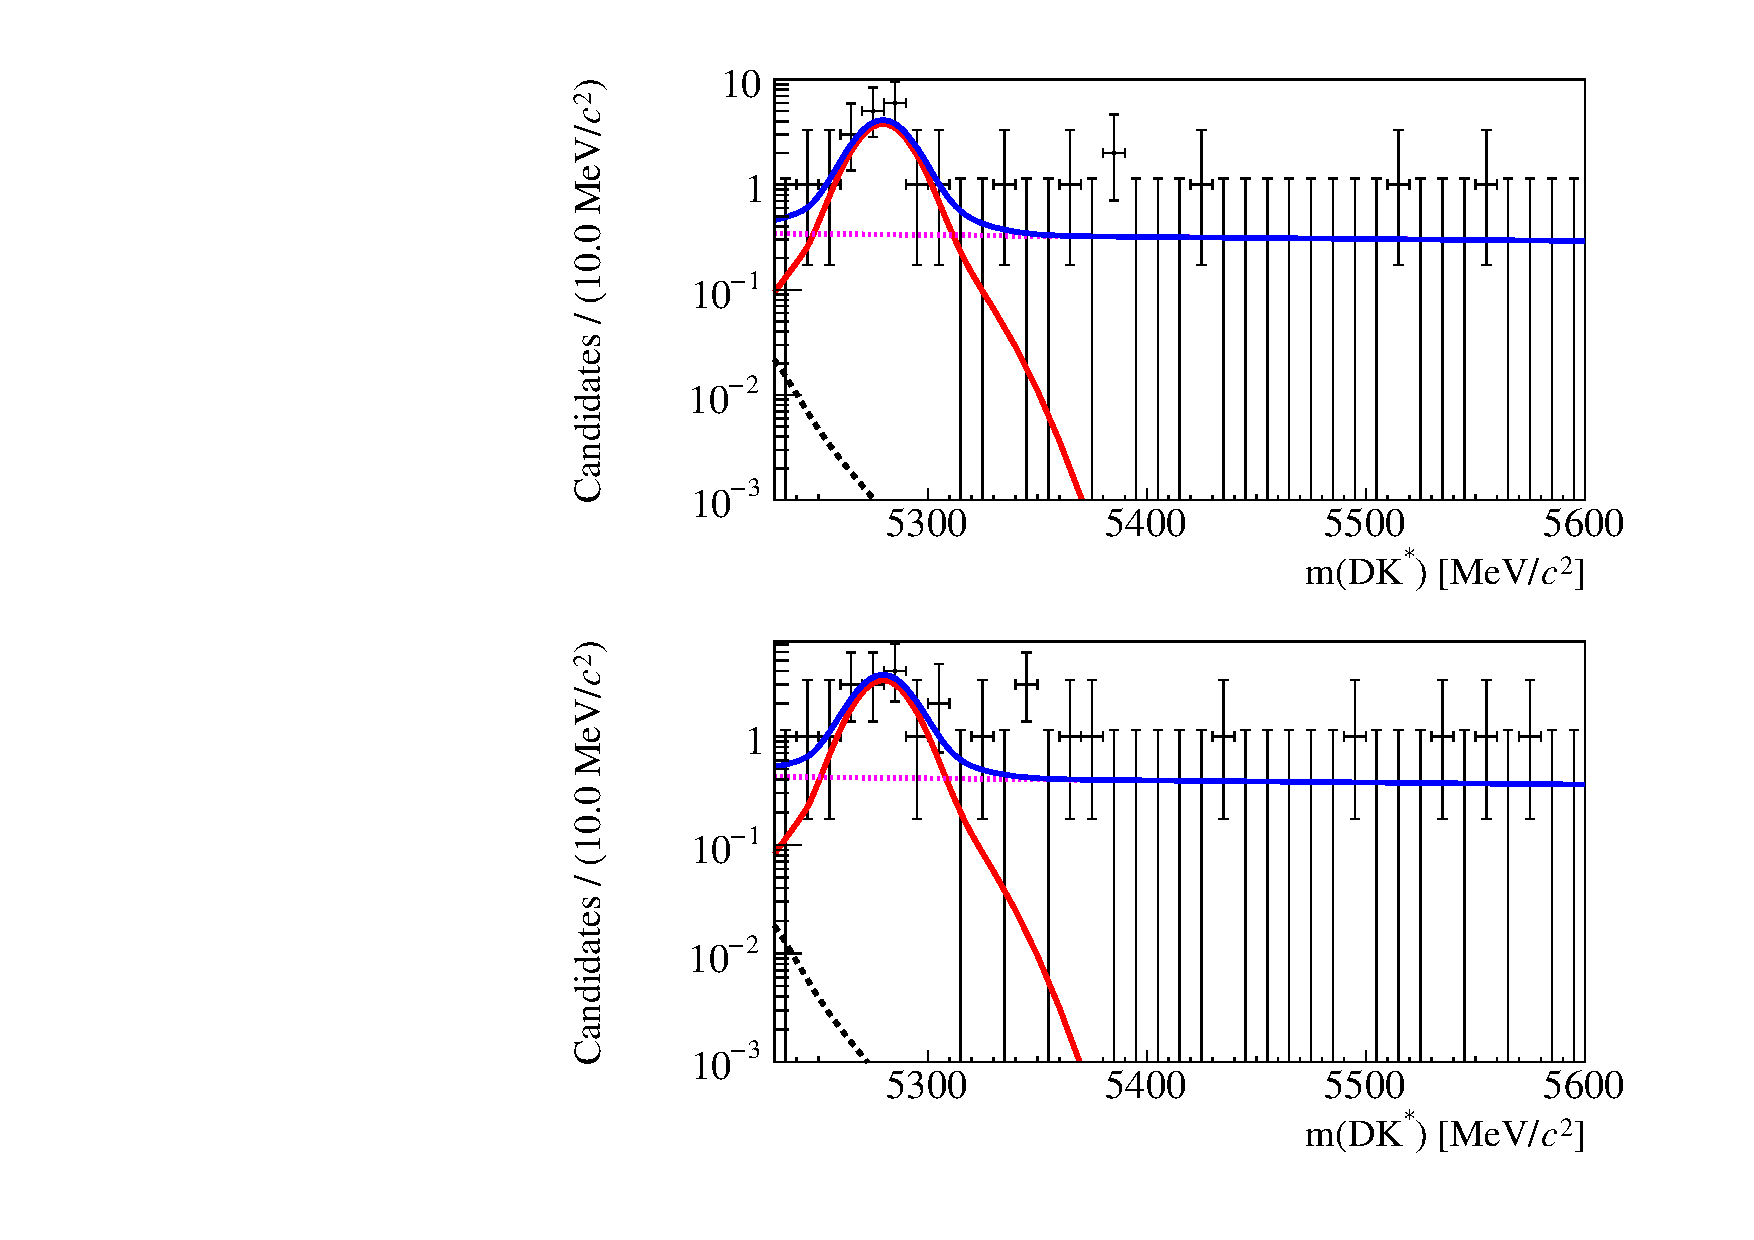
\includegraphics[width=0.3\linewidth]{figures/results/canvaslog_d2pipipipi_LL_run2_log.pdf}}
\hfill
\subfloat[$\pi K\pi\pi$, LL]{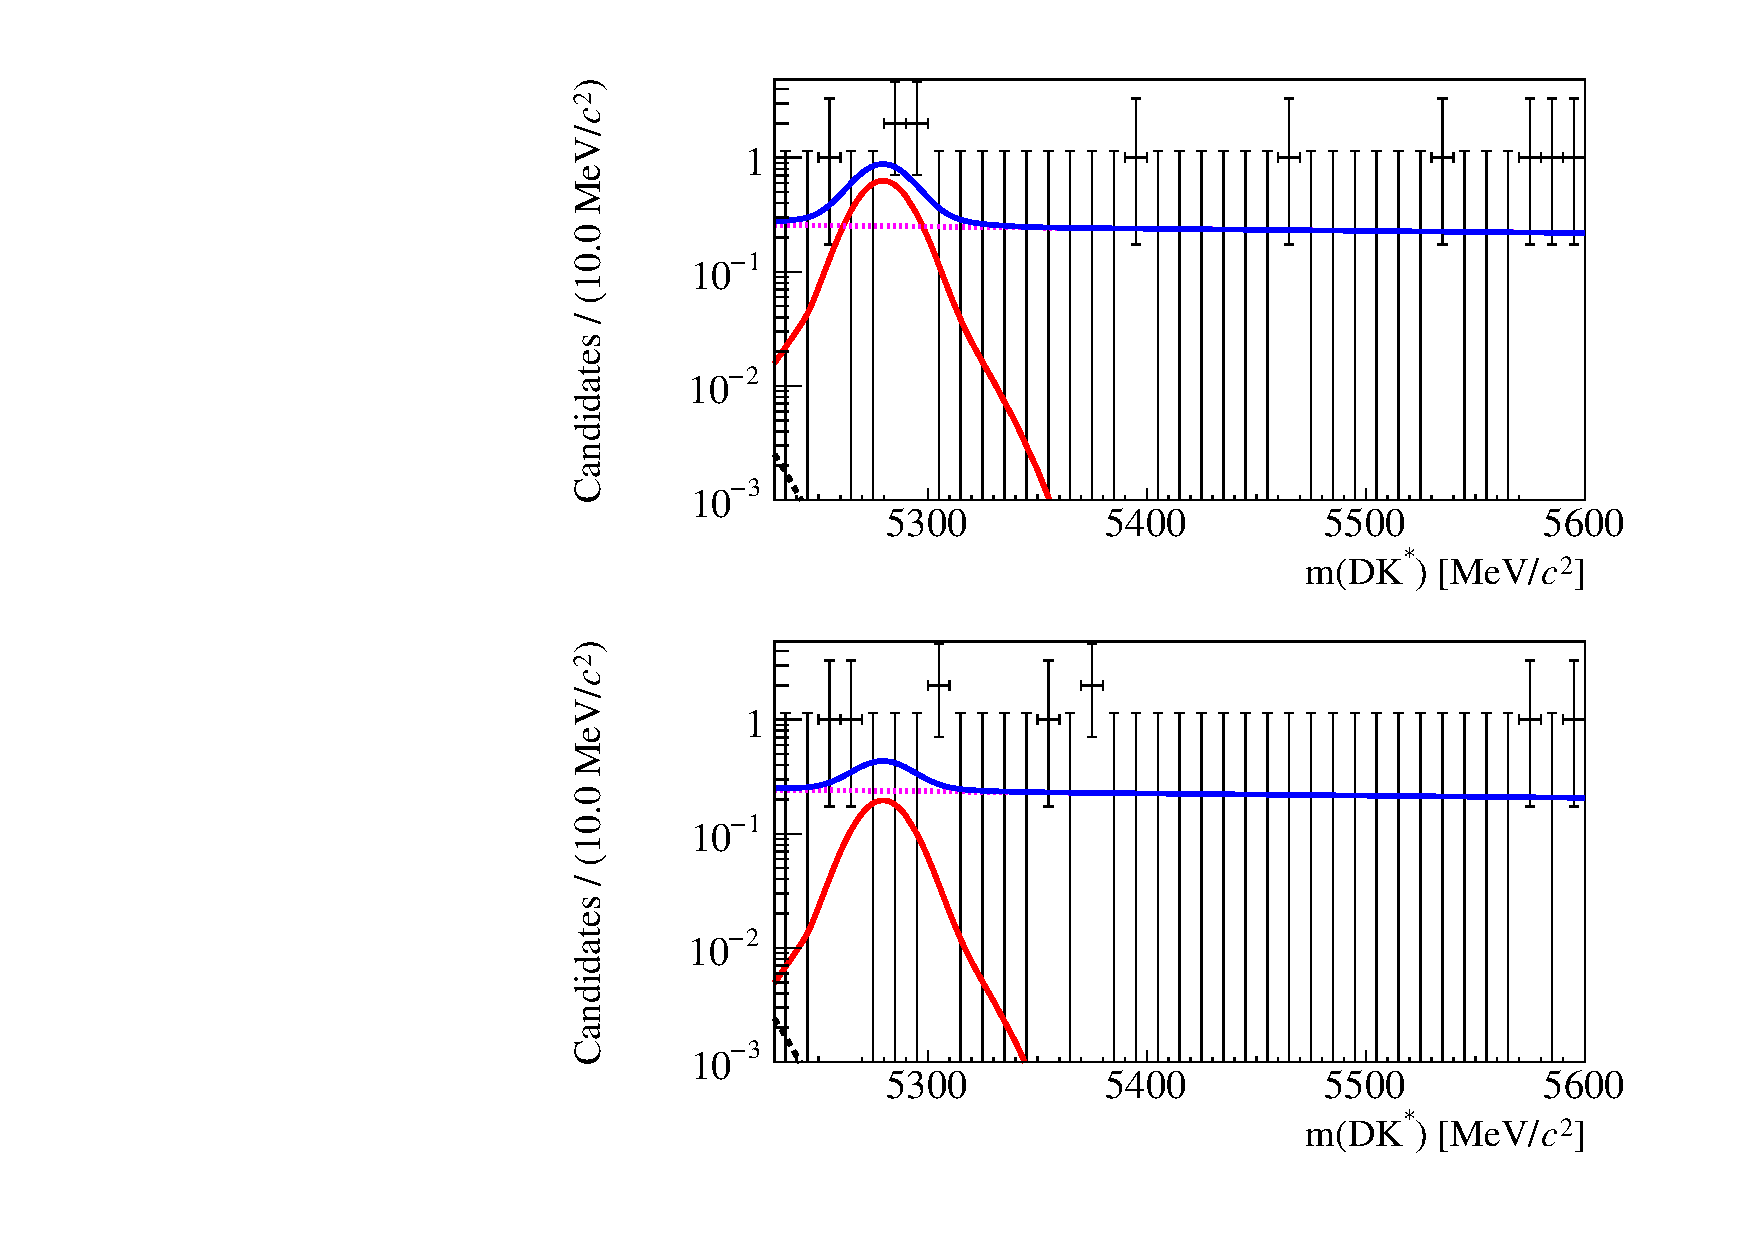
\includegraphics[width=0.3\linewidth]{figures/results/canvaslog_d2pikpipi_LL_run2_log.pdf}}
\hfill
\subfloat[$K\pi\pi\pi$, DD]{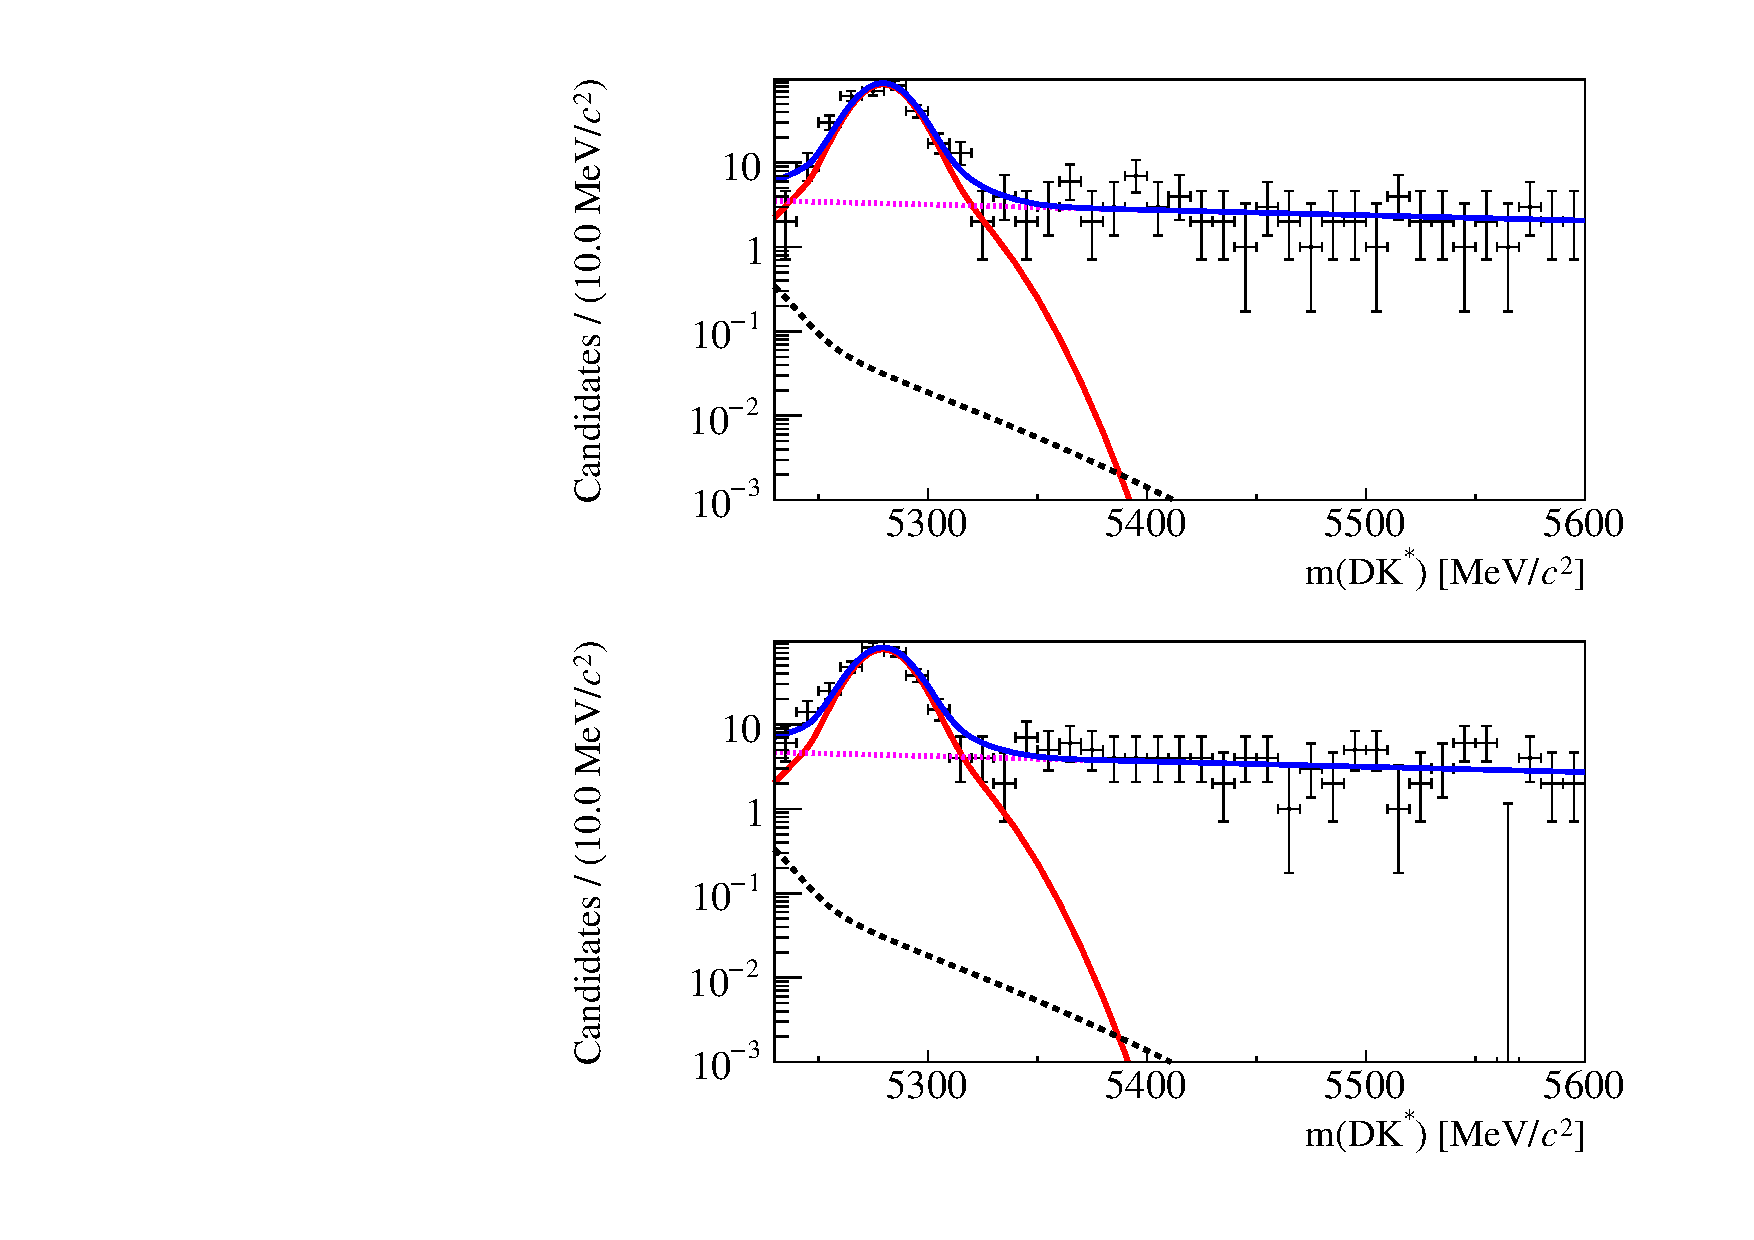
\includegraphics[width=0.3\linewidth]{figures/results/canvaslog_d2kpipipi_DD_run2_log.pdf}}
\hfill
\subfloat[$\pi\pi\pi\pi$, DD]{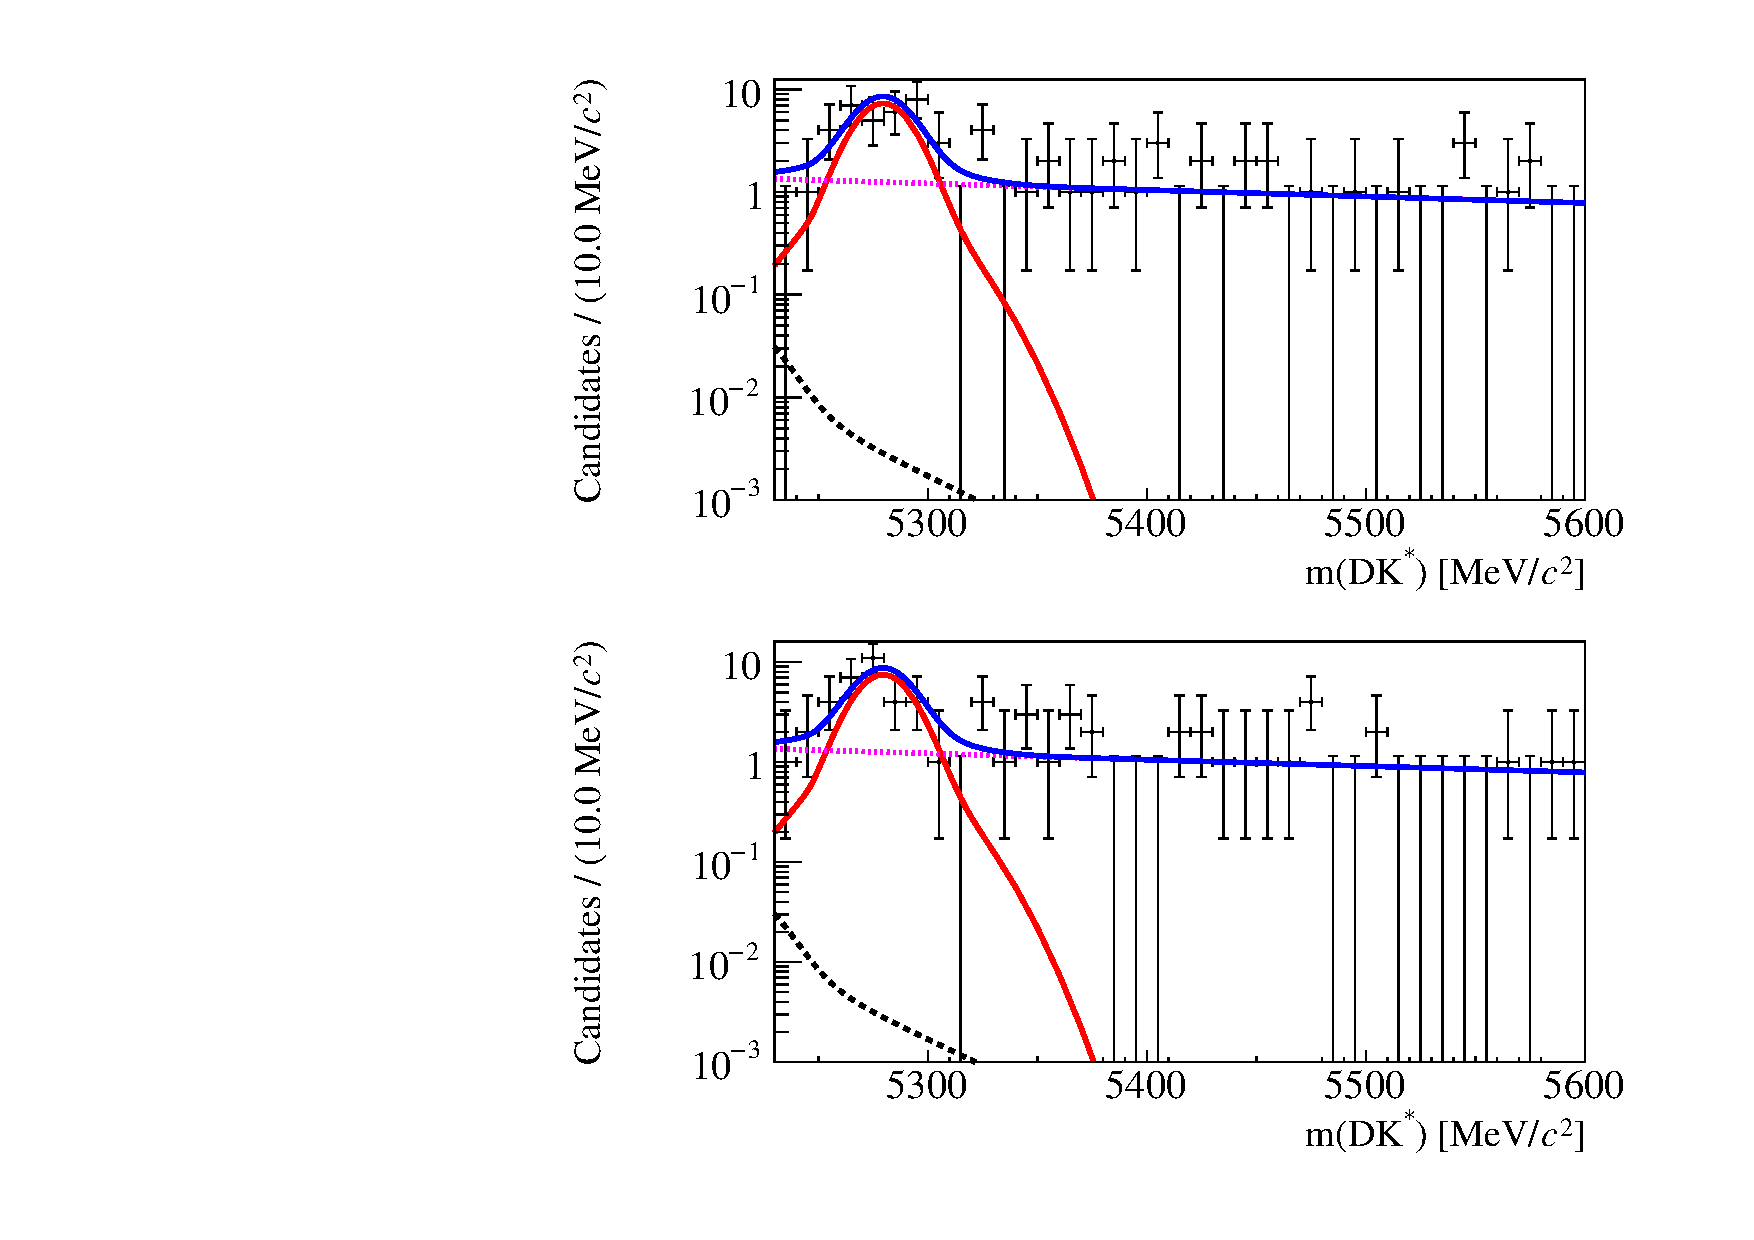
\includegraphics[width=0.3\linewidth]{figures/results/canvaslog_d2pipipipi_DD_run2_log.pdf}}
\hfill
\subfloat[$\pi K\pi\pi$, DD]{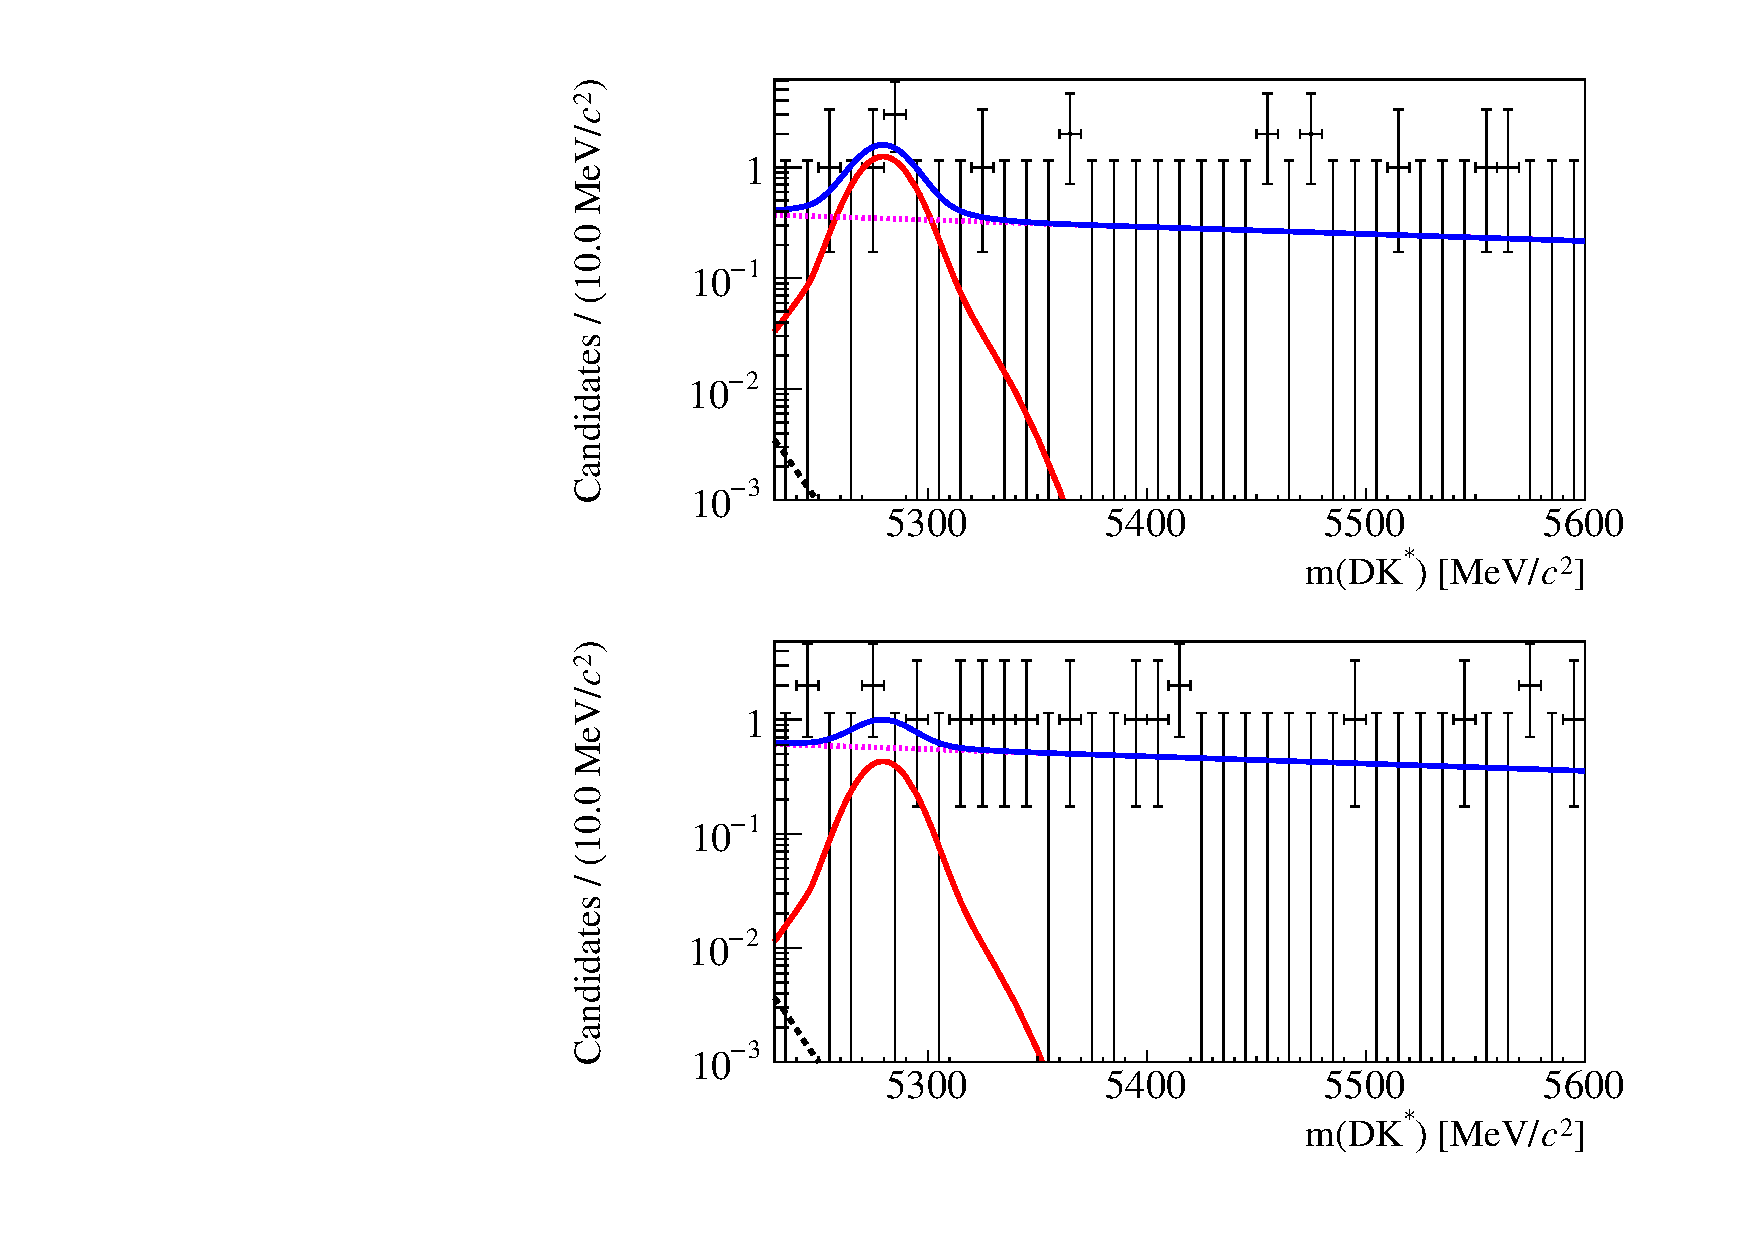
\includegraphics[width=0.3\linewidth]{figures/results/canvaslog_d2pikpipi_DD_run2_log.pdf}}
\caption{Results of the simultaneous fit for Run 1 data for 4-body modes. In each pair the top plot is for \Bp decays and the bottom plot is for \Bm decays.}
\label{datafit4bodyRun2}
\end{sidewaysfigure}

\clearpage

\section{Partially reconstructed yield in \CP fit}
\label{sec:app:partrecoyields}

Table \ref{partrecofixedyields} shows the fixed values of the total partially reconstructed yield in the \CP fit.

\begin{table}[h]
\centering
\begin{tabular}{c|cc|cc}
\hline
& \multicolumn{2}{c}{Run 1} & \multicolumn{2}{c}{Run 2} \\
& LL & DD & LL & DD \\
\hline
$K\pi$ & 0.55 & 1.03 & 1.18 & 1.35 \\
$KK$ & 0.060 & 0.112 & 0.116 & 0.131 \\
$\pi\pi$ & 0.019 & 0.034 & 0.041 & 0.049 \\
$\pi K$ & 0.008 & 0.012 & 0.017 & 0.016 \\
$K\pi\pi\pi$ & 0.34 & 0.52 & 0.55 & 1.31 \\
$\pi\pi\pi\pi$ & 0.031 & 0.045 & 0.050 & 0.122  \\
$\pi K\pi\pi$ & 0.004 & 0.006 & 0.007 & 0.014 \\
\hline
\end{tabular}
\caption{Partially reconstructed yields fixed in the \CP fit. The values show \Bp and \Bm combined, therefore half of the number shown is the fixed yield in the \Bp and \Bm categories separately. Uncertainties for these values are O(10\%)}
\label{partrecofixedyields}
\end{table}

\clearpage

\section{\CP fit results- combinatoric yields}
\label{sec:app:cpfit}

Table \ref{cpfitresultscomb} shows the fit results for all the combintoric yields.

\begin{table}[h]
\centering
{\tiny
\begin{tabular}{cccc}
Parameter & Fitted value & Negative error & Positive error \\
\hline
n\_comb\_d2kk\_minus\_DD\_run1 & $9.2644$ & $-3.2413$ & $4.1306$ \\
n\_comb\_d2kk\_minus\_DD\_run2 & $29.5912$ & $-5.8248$ & $6.6312$ \\
n\_comb\_d2kk\_minus\_LL\_run1 & $0.0000$ & $0.0000$ & $0.8409$ \\
n\_comb\_d2kk\_minus\_LL\_run2 & $10.2769$ & $-3.2586$ & $4.0635$ \\
n\_comb\_d2kk\_plus\_DD\_run1 & $11.0377$ & $-3.2611$ & $4.0359$ \\
n\_comb\_d2kk\_plus\_DD\_run2 & $28.5043$ & $-5.6729$ & $6.4917$ \\
n\_comb\_d2kk\_plus\_LL\_run1 & $6.9477$ & $-2.7573$ & $3.6031$ \\
n\_comb\_d2kk\_plus\_LL\_run2 & $4.1843$ & $-1.9720$ & $2.8582$ \\
n\_comb\_d2kpi\_minus\_DD\_run1 & $54.6504$ & $-8.3230$ & $9.2240$ \\
n\_comb\_d2kpi\_minus\_DD\_run2 & $155.8847$ & $-14.5137$ & $15.4315$ \\
n\_comb\_d2kpi\_minus\_LL\_run1 & $7.9888$ & $-2.8410$ & $3.7060$ \\
n\_comb\_d2kpi\_minus\_LL\_run2 & $15.9239$ & $-4.2968$ & $5.2111$ \\
n\_comb\_d2kpi\_plus\_DD\_run1 & $64.6413$ & $-9.1168$ & $10.0035$ \\
n\_comb\_d2kpi\_plus\_DD\_run2 & $154.8678$ & $-14.5472$ & $15.4779$ \\
n\_comb\_d2kpi\_plus\_LL\_run1 & $13.0412$ & $-3.8827$ & $4.7734$ \\
n\_comb\_d2kpi\_plus\_LL\_run2 & $19.8632$ & $-4.8676$ & $5.7870$ \\
n\_comb\_d2kpipipi\_minus\_DD\_run1 & $43.3016$ & $-7.2924$ & $8.1779$ \\
n\_comb\_d2kpipipi\_minus\_DD\_run2 & $135.8805$ & $-13.5205$ & $14.4923$ \\
n\_comb\_d2kpipipi\_minus\_LL\_run1 & $1.2423$ & $-0.8669$ & $1.6936$ \\
n\_comb\_d2kpipipi\_minus\_LL\_run2 & $9.5762$ & $-3.1916$ & $4.1240$ \\
n\_comb\_d2kpipipi\_plus\_DD\_run1 & $26.9317$ & $-5.7903$ & $6.6844$ \\
n\_comb\_d2kpipipi\_plus\_DD\_run2 & $99.1967$ & $-11.8452$ & $12.8635$ \\
n\_comb\_d2kpipipi\_plus\_LL\_run1 & $3.2506$ & $-1.7378$ & $2.6474$ \\
n\_comb\_d2kpipipi\_plus\_LL\_run2 & $13.2367$ & $-3.9555$ & $4.9514$ \\
n\_comb\_d2pik\_minus\_DD\_run1 & $4.9988$ & $-1.9166$ & $2.5806$ \\
n\_comb\_d2pik\_minus\_DD\_run2 & $22.0339$ & $-4.6793$ & $5.3881$ \\
n\_comb\_d2pik\_minus\_LL\_run1 & $5.7087$ & $-2.1669$ & $2.8313$ \\
n\_comb\_d2pik\_minus\_LL\_run2 & $8.7460$ & $-2.6869$ & $3.3592$ \\
n\_comb\_d2pik\_plus\_DD\_run1 & $3.5811$ & $-1.7805$ & $2.5381$ \\
n\_comb\_d2pik\_plus\_DD\_run2 & $18.5923$ & $-4.4531$ & $5.1798$ \\
n\_comb\_d2pik\_plus\_LL\_run1 & $6.2716$ & $-2.3435$ & $3.0760$ \\
n\_comb\_d2pik\_plus\_LL\_run2 & $10.1699$ & $-3.0098$ & $3.7295$ \\
n\_comb\_d2pikpipi\_minus\_DD\_run1 & $2.3189$ & $-1.2711$ & $1.9952$ \\
n\_comb\_d2pikpipi\_minus\_DD\_run2 & $17.6630$ & $-4.0703$ & $4.7570$ \\
n\_comb\_d2pikpipi\_minus\_LL\_run1 & $2.8918$ & $-1.4152$ & $2.0824$ \\
n\_comb\_d2pikpipi\_minus\_LL\_run2 & $8.0364$ & $-2.7499$ & $3.4109$ \\
n\_comb\_d2pikpipi\_plus\_DD\_run1 & $8.5916$ & $-2.7559$ & $3.4576$ \\
n\_comb\_d2pikpipi\_plus\_DD\_run2 & $11.3239$ & $-3.2068$ & $3.9408$ \\
n\_comb\_d2pikpipi\_plus\_LL\_run1 & $0.5468$ & $0.0000$ & $1.5795$ \\
n\_comb\_d2pikpipi\_plus\_LL\_run2 & $8.1112$ & $-2.7664$ & $3.5289$ \\
n\_comb\_d2pipi\_minus\_DD\_run1 & $2.5555$ & $-1.3991$ & $2.1909$ \\
n\_comb\_d2pipi\_minus\_DD\_run2 & $22.3622$ & $-5.1858$ & $6.0198$ \\
n\_comb\_d2pipi\_minus\_LL\_run1 & $2.8497$ & $-1.5111$ & $2.2778$ \\
n\_comb\_d2pipi\_minus\_LL\_run2 & $4.5092$ & $-1.8921$ & $2.6286$ \\
n\_comb\_d2pipi\_plus\_DD\_run1 & $6.3000$ & $-2.4807$ & $3.2589$ \\
n\_comb\_d2pipi\_plus\_DD\_run2 & $20.7800$ & $-4.7887$ & $5.5926$ \\
n\_comb\_d2pipi\_plus\_LL\_run1 & $1.2180$ & $-0.8483$ & $1.6131$ \\
n\_comb\_d2pipi\_plus\_LL\_run2 & $4.4715$ & $-1.9438$ & $2.6960$ \\
n\_comb\_d2pipipipi\_minus\_DD\_run1 & $6.4229$ & $-2.4483$ & $3.2700$ \\
n\_comb\_d2pipipipi\_minus\_DD\_run2 & $39.6563$ & $-6.6510$ & $7.4336$ \\
n\_comb\_d2pipipipi\_minus\_LL\_run1 & $4.4140$ & $-1.9854$ & $2.7711$ \\
n\_comb\_d2pipipipi\_minus\_LL\_run2 & $14.1558$ & $-3.8758$ & $4.6747$ \\
n\_comb\_d2pipipipi\_plus\_DD\_run1 & $8.7170$ & $-3.0106$ & $3.8208$ \\
n\_comb\_d2pipipipi\_plus\_DD\_run2 & $38.6850$ & $-6.5763$ & $7.3661$ \\
n\_comb\_d2pipipipi\_plus\_LL\_run1 & $3.0998$ & $-1.4649$ & $2.1490$ \\
n\_comb\_d2pipipipi\_plus\_LL\_run2 & $9.5359$ & $-3.1792$ & $4.0340$ \\
\end{tabular}}
\caption{Fitted values of all the combinatoric yields from the \CP fit}
\label{cpfitresultscomb}
\end{table}

\clearpage

\section{CF and ADS combinatoric}
\label{sec:app:combinatoric}


%\subsection{Inspection of the full spectrum of the favoured mode}
\subsection{Comparison of the sideband in the CF and ADS mode}

In the analysis the decay of interest, \decay{\Bm}{\D(\Km_{1}\pip_{2})\Kstarm(\KS(\pip_{4}\pim_{5})\pim_{3})} has a five body final state. The numbers in subscripts refer to the label given to the particles when calculating the various mass combinations, which are used in all the figures in this section to identify the invariant mass sum to which each plot corresponds. 

%These plots have a number of interesting features and in general are not smooth. Some resonances are easy to identify - others less so. Interesting features are that twoBody24\_M and twoBody25\_M look very similar. These are composed of the pion from the \D and one of the pion from the \KS. twoBody24\_M is same sign while twoBody25\_M is opposite sign. The lack of difference here suggests no resonances. Taking combinations with the bachelor pion and one of the \KS pions has a similar result. This is unsurprising since the \KS selection requirements on decay flight mean that these pairs of pions are not originating from the same place.
%
%The three body combinations show more structure. threeBody123\_M combines all particles except the \KS. This double hump structure is expected since what is being plotted is the partially reconstructed B mass with a missing scalar daughter of a vector particle. The humps are not equal in size due to the reconstruction efficiency of the \KS as a function of momentum. The threebody345\_M plots the combination of the \Kstarm. Hence the narrow peak is the \Kstarm, but the higher excited kaon resonance can be seen around 1430 and then the \Dp is also visible. Note that in the selection most of the events are removed since they are not compatible with the $K^{*-}(892)$ selection.
%
%The combination of all pions could show a mean at the \D mass for the \decay{\D}{\KS\pi\pi} decay. While some small bump is present in the LL candidates, this decay mode is also checked in simulation with full selection applied, and the yield is negligible.
%
%Hence inspection in the favoured mode has been rather inconclusive to see any strong resonances appearing in other combinations of tracks. 



Comparisons of various invariant mass distributions are made between the background in the Cabibbo favoured decay and the supressed decay for Run 1 and Run 2 data combined. The comparisons look at the high B mass region ($>$ 5400 \mev) with the full selection applied, except the BDT selection in the ADS mode is relaxed to match the CF mode and the double misID veto is applied to both modes to allow fairer comparison. Also, the \Kstar selection is loosened to leave enough events to make a reasonable comparison. In each case particle 1 is the kaon and the rest are pions. 

Drawing various invariant mass distributions like this when there are down tracks in the sample included is not trivial. In DaVinci track momenta are provided at the first state. For long tracks this is very similar to the momenta of the track at the point of production, but this is not the case for downstream tracks. Hence for real \KS combining the momenta of the pions in the tuple leads to a much broader \KS mass in comparison to if the combination is made within DaVinci where the track momenta are propagated to the point of decay, and hence the variable $Ks\_M$ in the tuple has the expected resolution. This means that when searching for light resonances with downstream track one should expect some signigicant smearing since if there was a true $\rho$ the momenta of the tracks in the tuple are not recorded at that point, and hence won't form a nice peak. Due to this complication the invariant mass distributions are shown using both the track momenta as given in the standard tuple at the first track state (non-DTF) and using the decay-tree-fit (DTF) momenta which means that the downstream momenta are that at the point of the \KS candidate decay. 

Figures \ref{projections2bodydtf} and \ref{projections3bodydtf} show all the possible 2 and 3 body combinations of invariant mass sum of these final state particles using DTF momenta. The \Kstar candidates are required to be within 500 \mev of the nominal mass, but no requirement is placed on the \KS helicity angle. This provides enough events for comparison, and attempts to keep the distributions closer to those in the actual selected data. Figures \ref{projections2bodynodtf}, \ref{projections3bodynodtf} and show the same invariant mass distributions, but using the non-DTF momenta.

The LL candidate distributions are consistent, but suffer from low statistics. Discrepancies are observed in the DD candidates is larger than for LL. Particular differences are between combinations one of the D daughters and the bachelor pion. Further large differences are seen in the combination of both D daughters and the bachelor pion and both D daughters plus one of the pions of the \KS. 

The distributions so far have a very wide \Kstar mass window, which results in most of the events not representing the final selection. In order to improve the comparison, Figure \ref{projectionstighter} shows all the possible 2 and 3 body combinations of invariant mass sum of these final state particles using DTF momenta, but this time with the \Kstar candidates are required to be within 200 \mev of the nominal mass and the \KS helicity angle selection is applied. This gives a more accurate comparison of the combinatoric in the final selection, but naturally results in fewer statistics. These distributions are only shown for the DD candidates as this is where the inconsistencies were observed and the LL candidate distributions simply would not yield enough statistics to provide any meaningful information. These plots do not have as significant discrepancies as those found in the distributions with the higher statistics (wider \Kstar mass window).

Figure \ref{projection4pions} shows two different 4-body combinations of the five final state particles using the DTF momenta. The plots compare both the looser \Kstar selection and tighter \Kstar selection. The same observations can be made for these distributions. There is a signifcant discrepancy between the CF and ADS mode distributions when looking at the combination of both D daughters plus both of the pions of the \KS with the loose \Kstar selection. However, when the tighter \Kstar selection is applied this distribution becomes more consistent and the discrepancy is no longer significant. 

From this we can conclude that the significant discrepancies observed in the higher statistics distributions are mainly due to the inclusion of candidates in the wider \Kstar region that do not occur in the final selection, therefore this is not the cause of the differences observed in the data in the fit. However, when the \Kstar selection is tightened there are still slight differences remaining in the distributions, but due to the lower statistics it is difficult to make any defininative statement about the cause of the discrepancy. The equivalent distributions have been made for the $K\pi\pi\pi$ mode and the same results are observed.

%Finally to look at the general purity of the D candidates the D mass distributions are plotted in Fig.~\ref{Dpurity}. In this case the selection used for charmless studies is used - otherwise this distribution is biased by the D mass constraint.
%
%These plots reveal two notable features. First, it seems that the relative amount of combinatoric D in the ADS mode is larger than for the CF mode. Secondly the proportion of real \Kstar seems higher in the ADS sideband compared to the CF mode. These show some differences between the composition of the sideband which must be responsible for the differences observed in the data fit.

In conclusion while some differences in these distributions do exist, it is not possible to draw any conclusions as to why the distributions are different. Furthermore, any conclusions drawn from these plots should be treated with great care since only a few percent of the data in these plots would pass the \Kstarm selection used in the analysis.   


\begin{figure}
\subfloat[LL candidates]{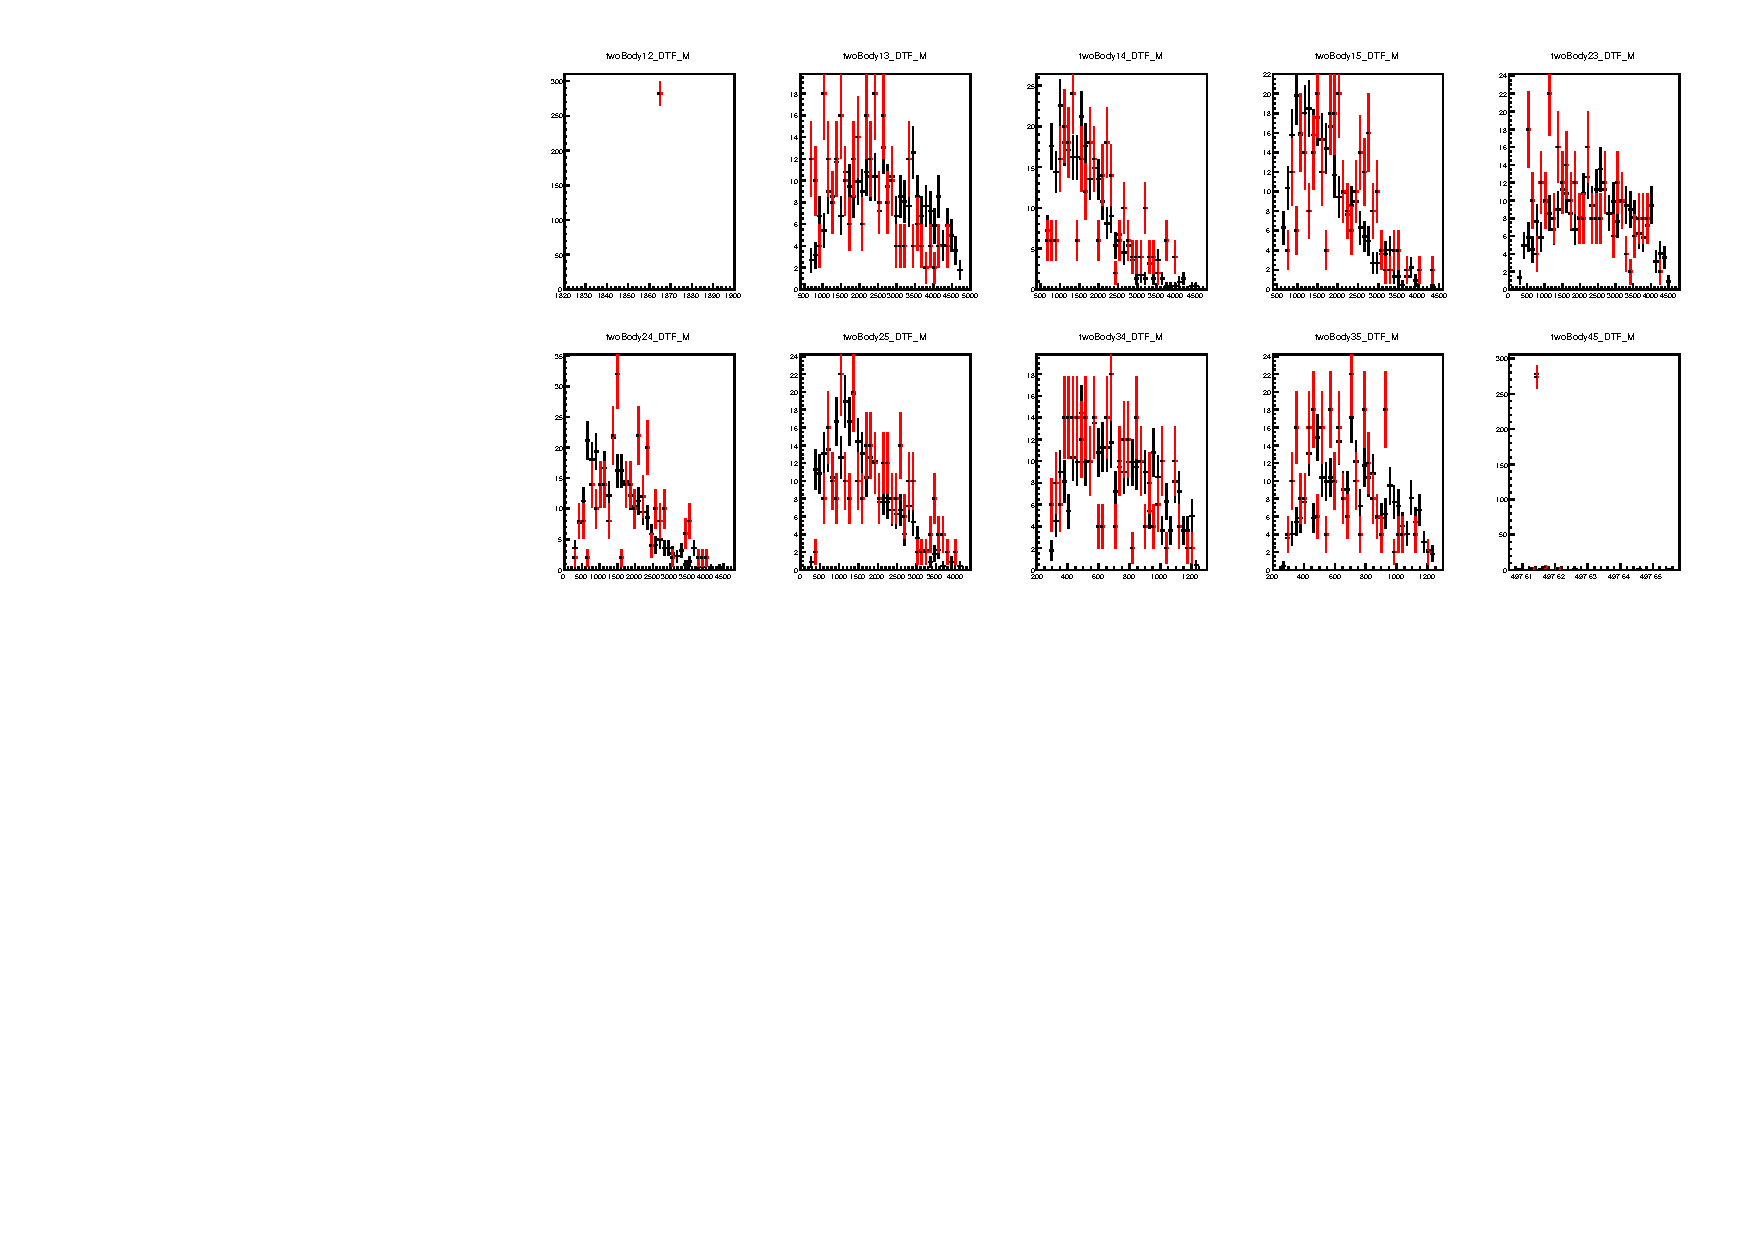
\includegraphics[width=\linewidth]{figures/massProjections/massProjectionsLL_2body_dtf.pdf}}
\hfill
\subfloat[DD candidates]{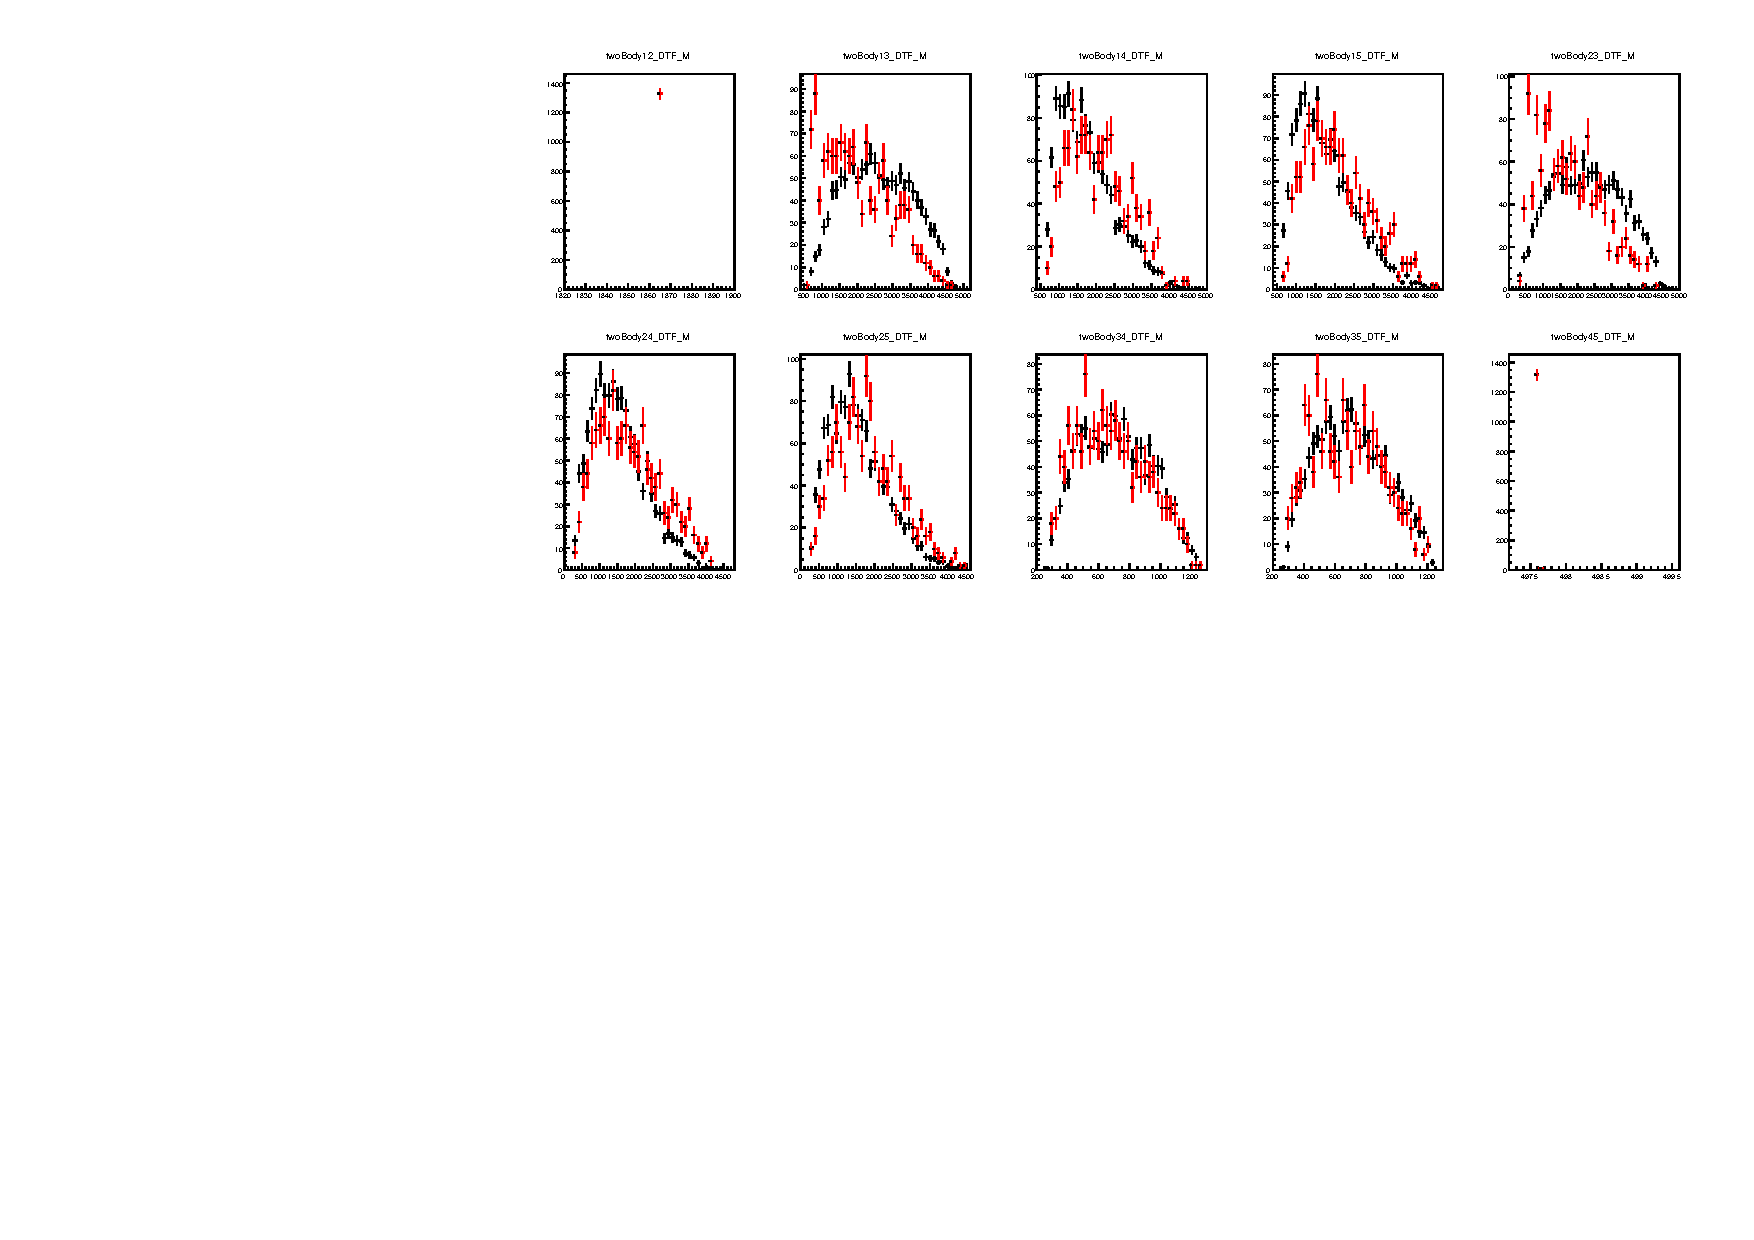
\includegraphics[width=\linewidth]{figures/massProjections/massProjectionsDD_2body_dtf.pdf}}
\caption{Invariant mass projections of all of the possible two body combinations of the five final state particles. Comparing \decay{\Dz}{\Km\pip} (black) and \decay{\Dz}{\Kp\pim} (red) using Run 1 and Run 2 data in the high B mass region ($>$ 5400 \mevcc) with the full selection, except for the \Kstar mass window is widened to 500 \mev and there is no \KS helicity angle requirement. Also, the tightened BDT cut in the ADS mode is not applied. The invariant mass combination 12 and 45 have been constrained to be the \Dz mass and \KS mass respectively.}
\label{projections2bodydtf}
\end{figure}

\begin{figure}
\subfloat[LL candidates]{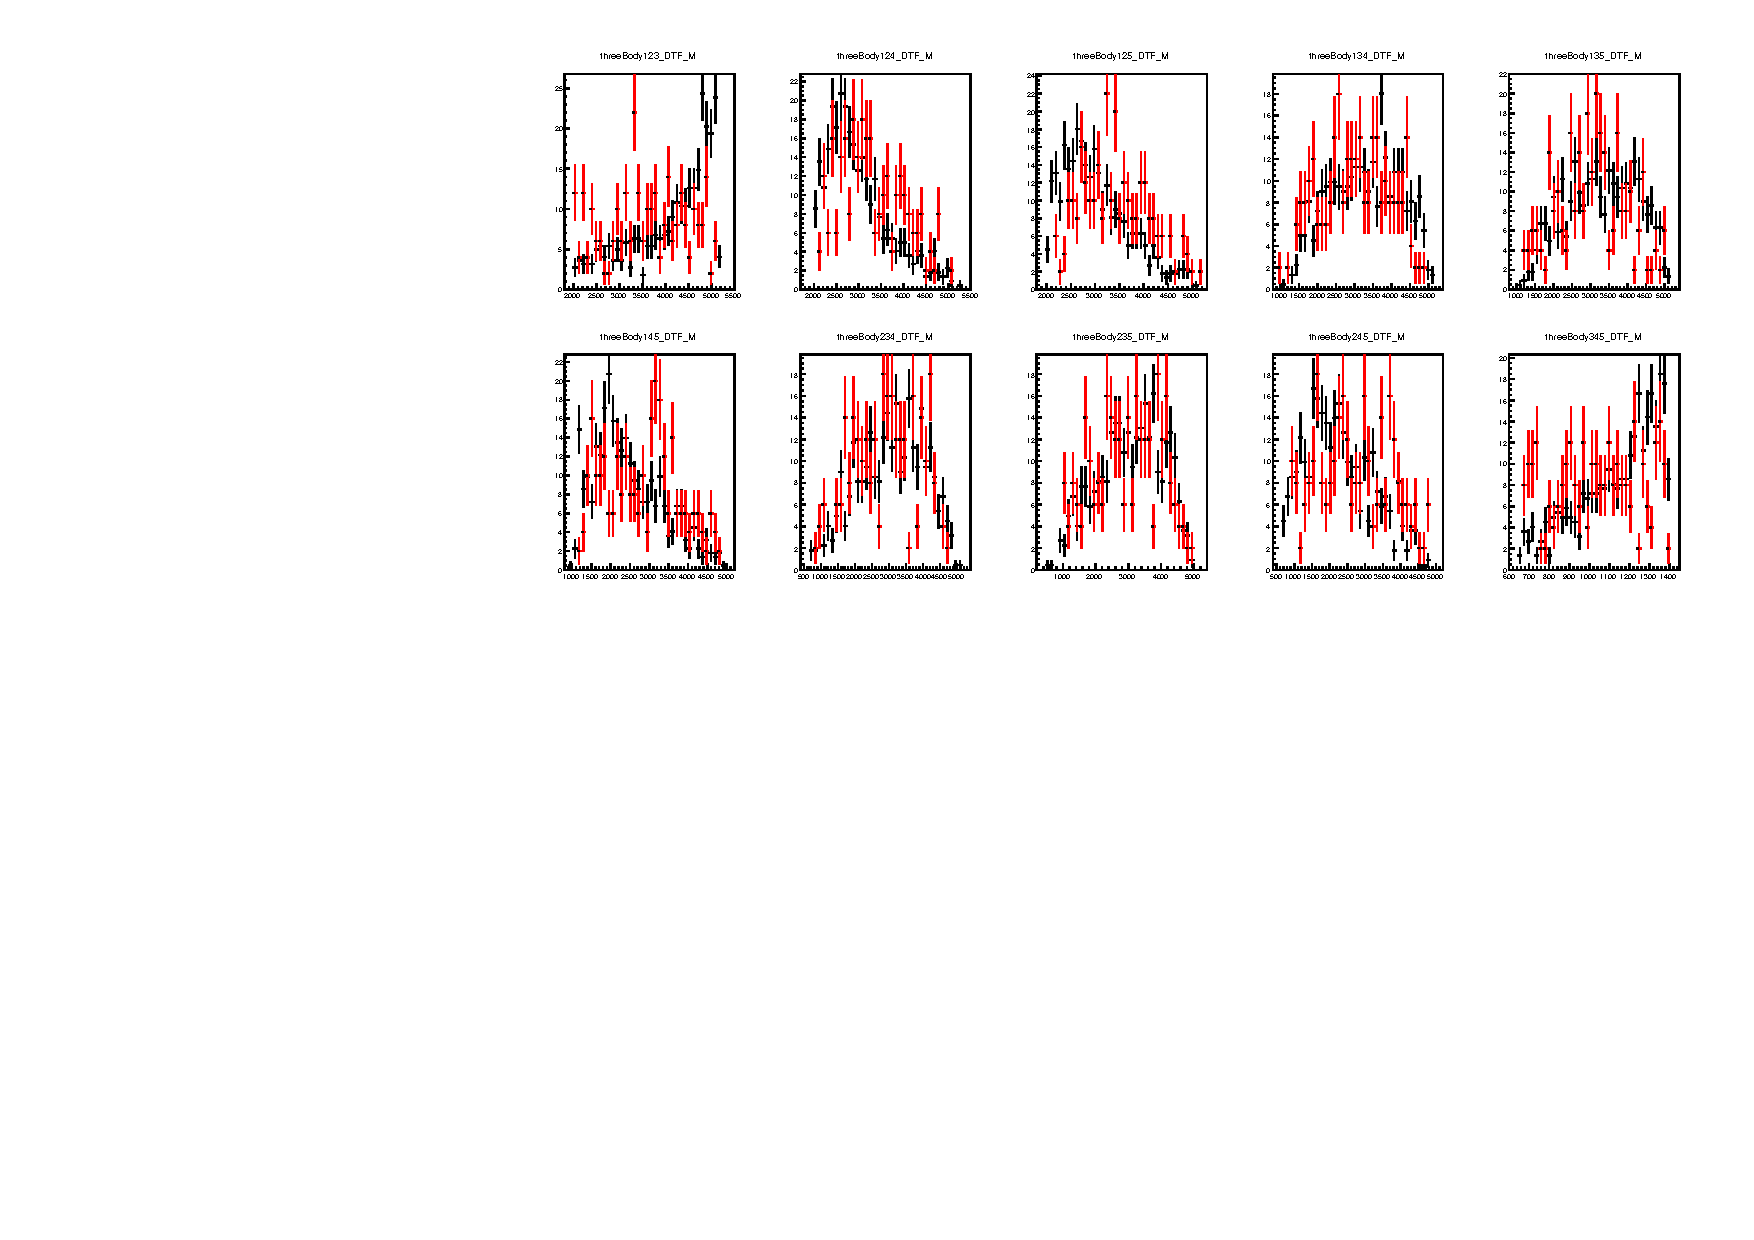
\includegraphics[width=\linewidth]{figures/massProjections/massProjectionsLL_3body_dtf.pdf}}
\hfill
\subfloat[DD candidates]{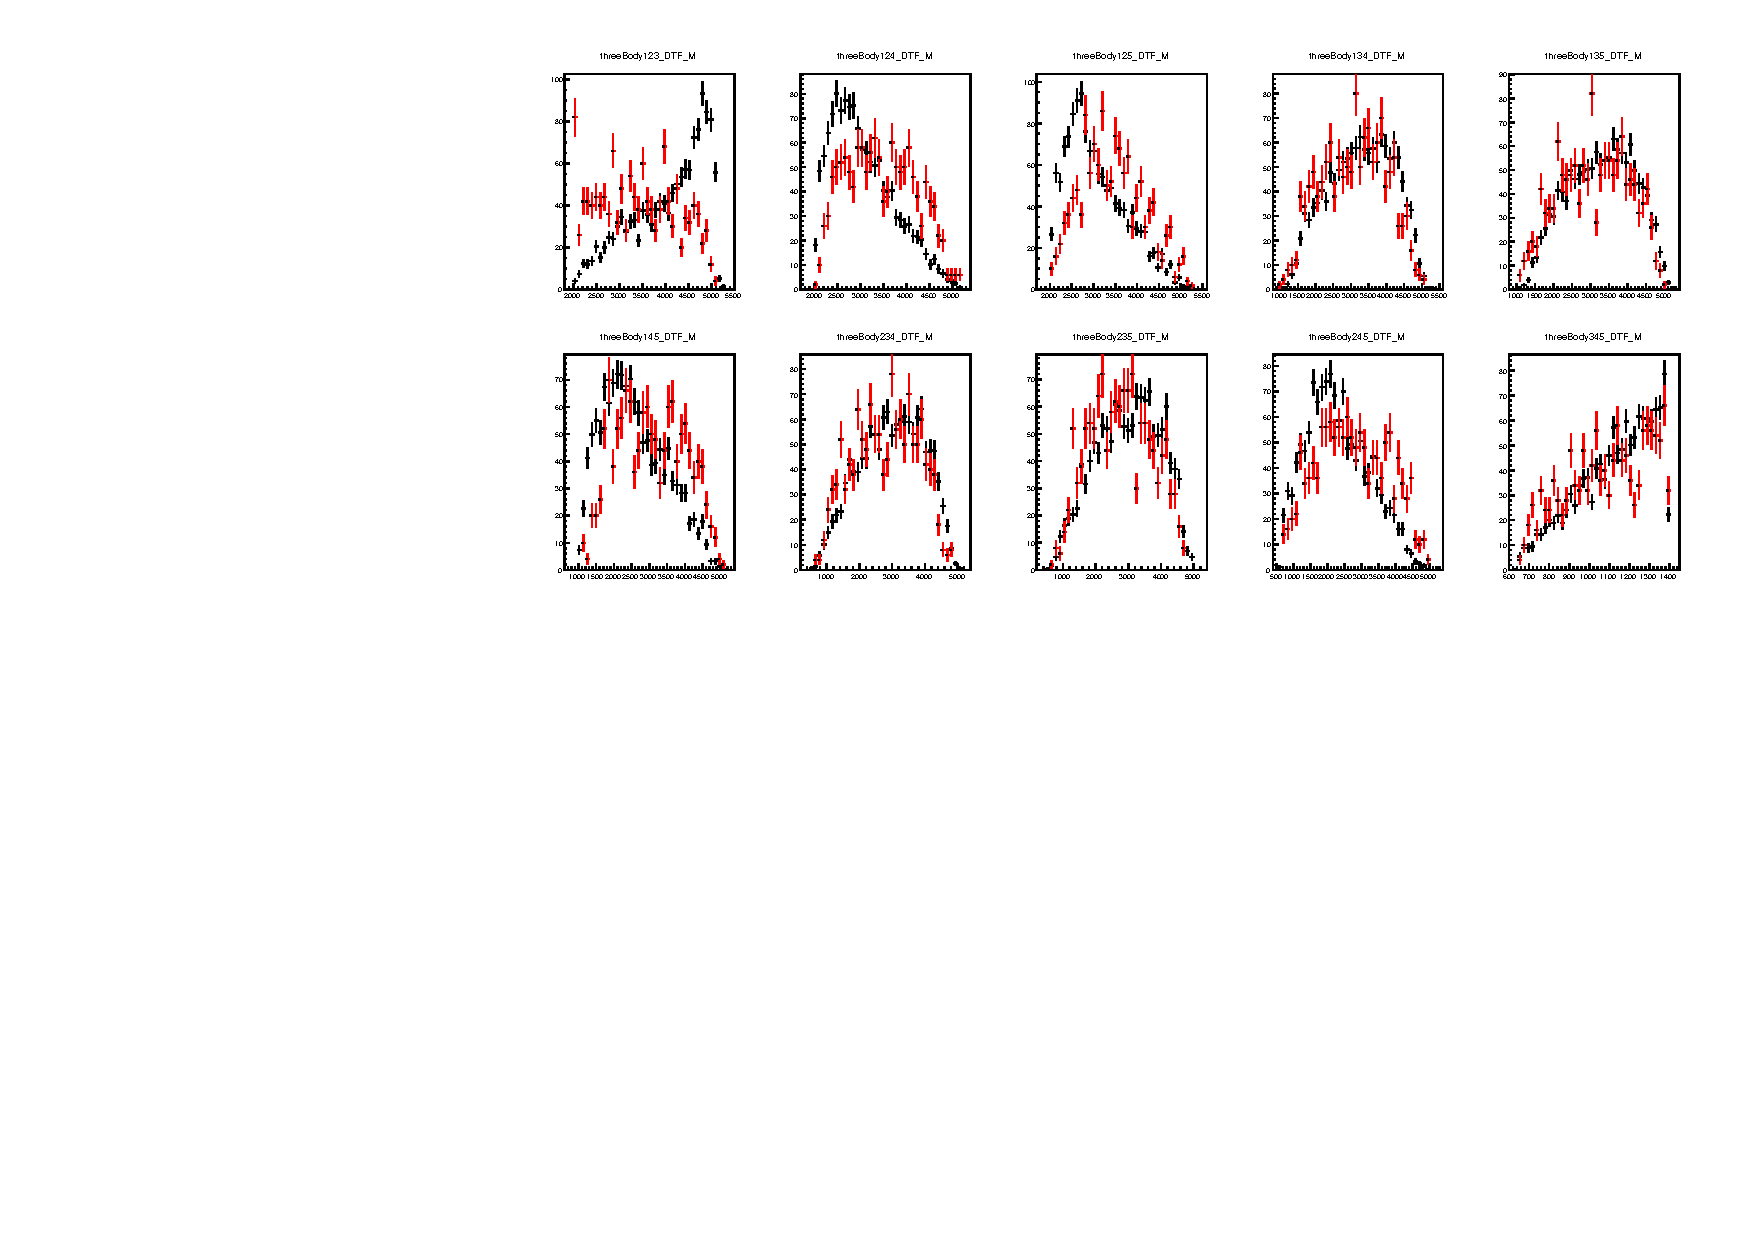
\includegraphics[width=\linewidth]{figures/massProjections/massProjectionsDD_3body_dtf.pdf}}
\caption{Invariant mass projections of all of the possible three body combinations of the five final state particles. Comparing \decay{\Dz}{\Km\pip} (black) and \decay{\Dz}{\Kp\pim} (red) using Run 1 and Run 2 data in the high B mass region ($>$ 5400 \mevcc) with the full selection, except for the \Kstar mass window is widened to 500 \mev and there is no \KS helicity angle requirement. Also, the tightened BDT cut in the ADS mode is not applied. The invariant mass combination 12 and 45 have been constrained to be the \Dz mass and \KS mass respectively.}
\label{projections3bodydtf}
\end{figure}

\begin{figure}
\subfloat[LL candidates]{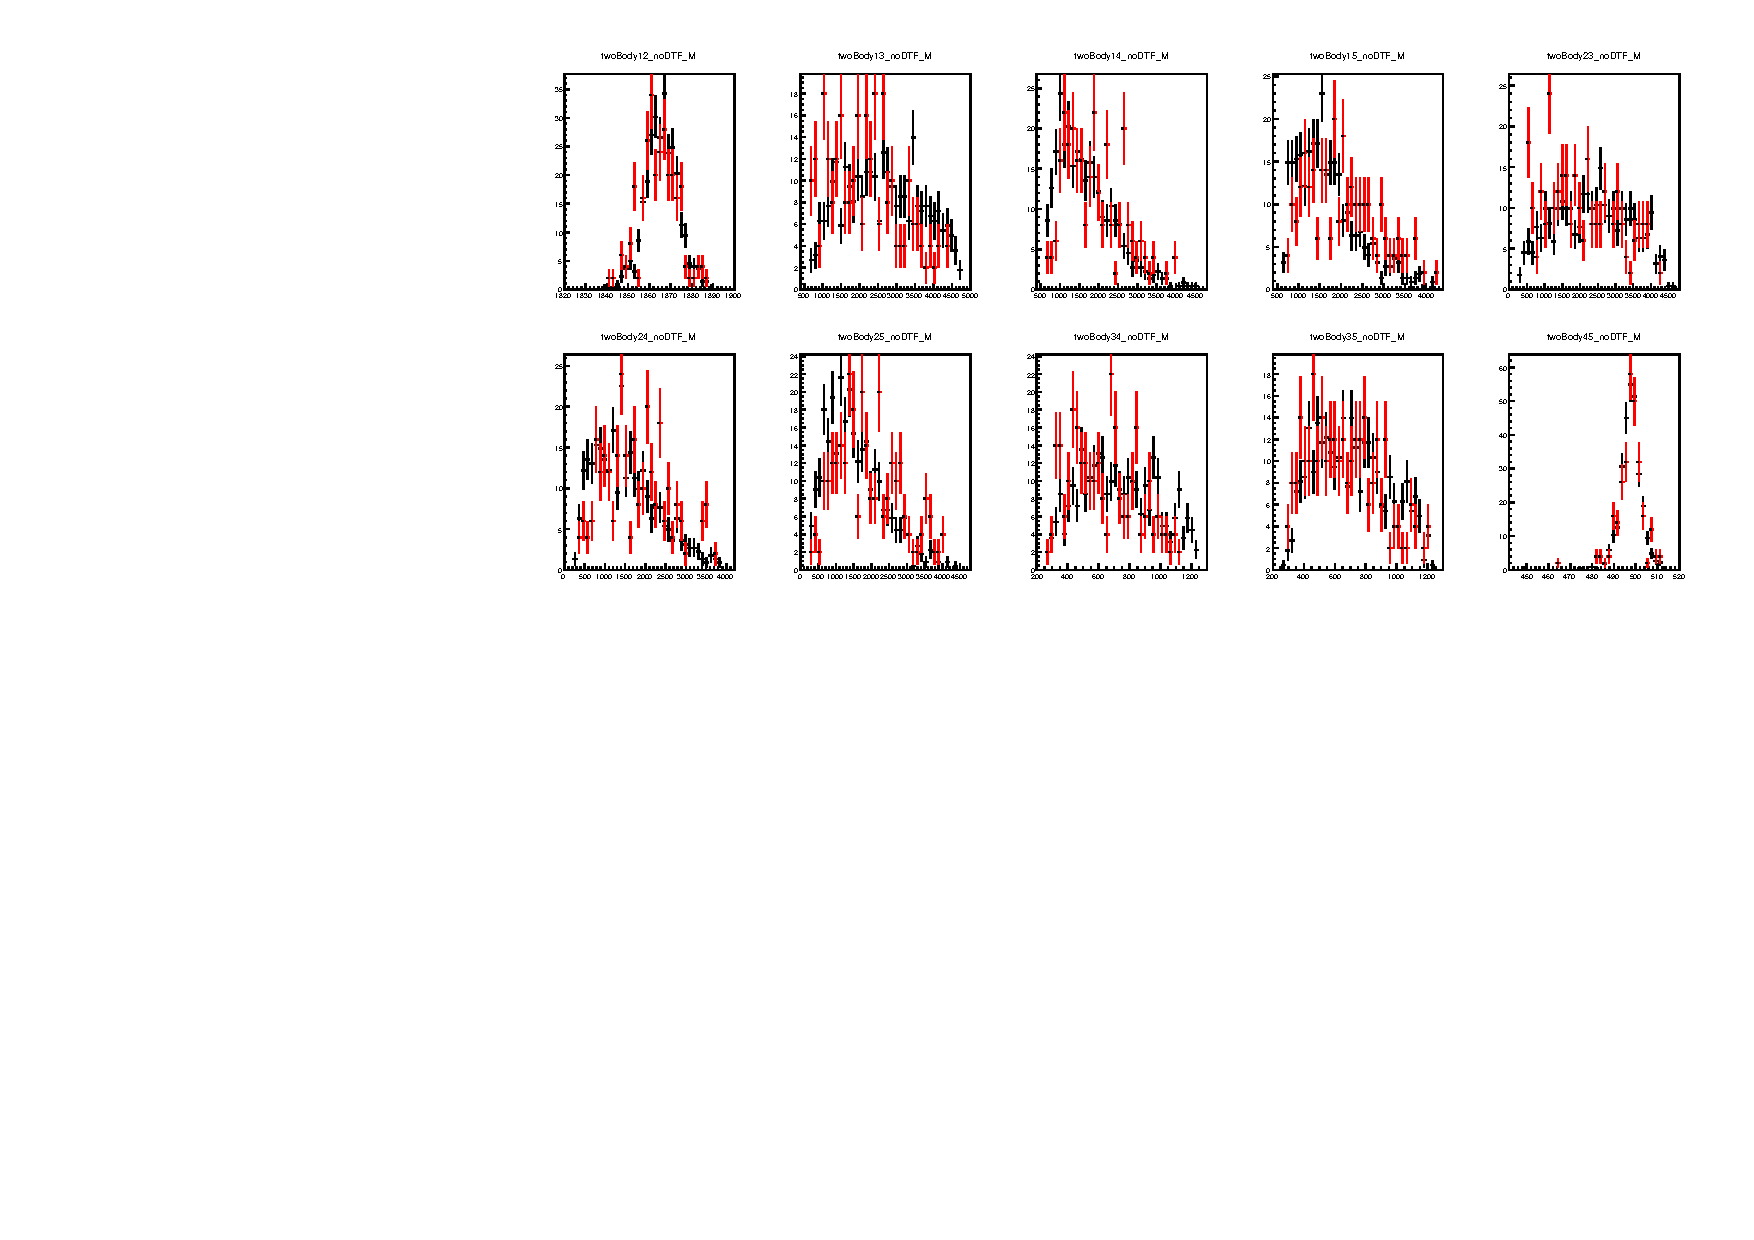
\includegraphics[width=\linewidth]{figures/massProjections/massProjectionsLL_2body_nodtf.pdf}}
\hfill
\subfloat[DD candidates]{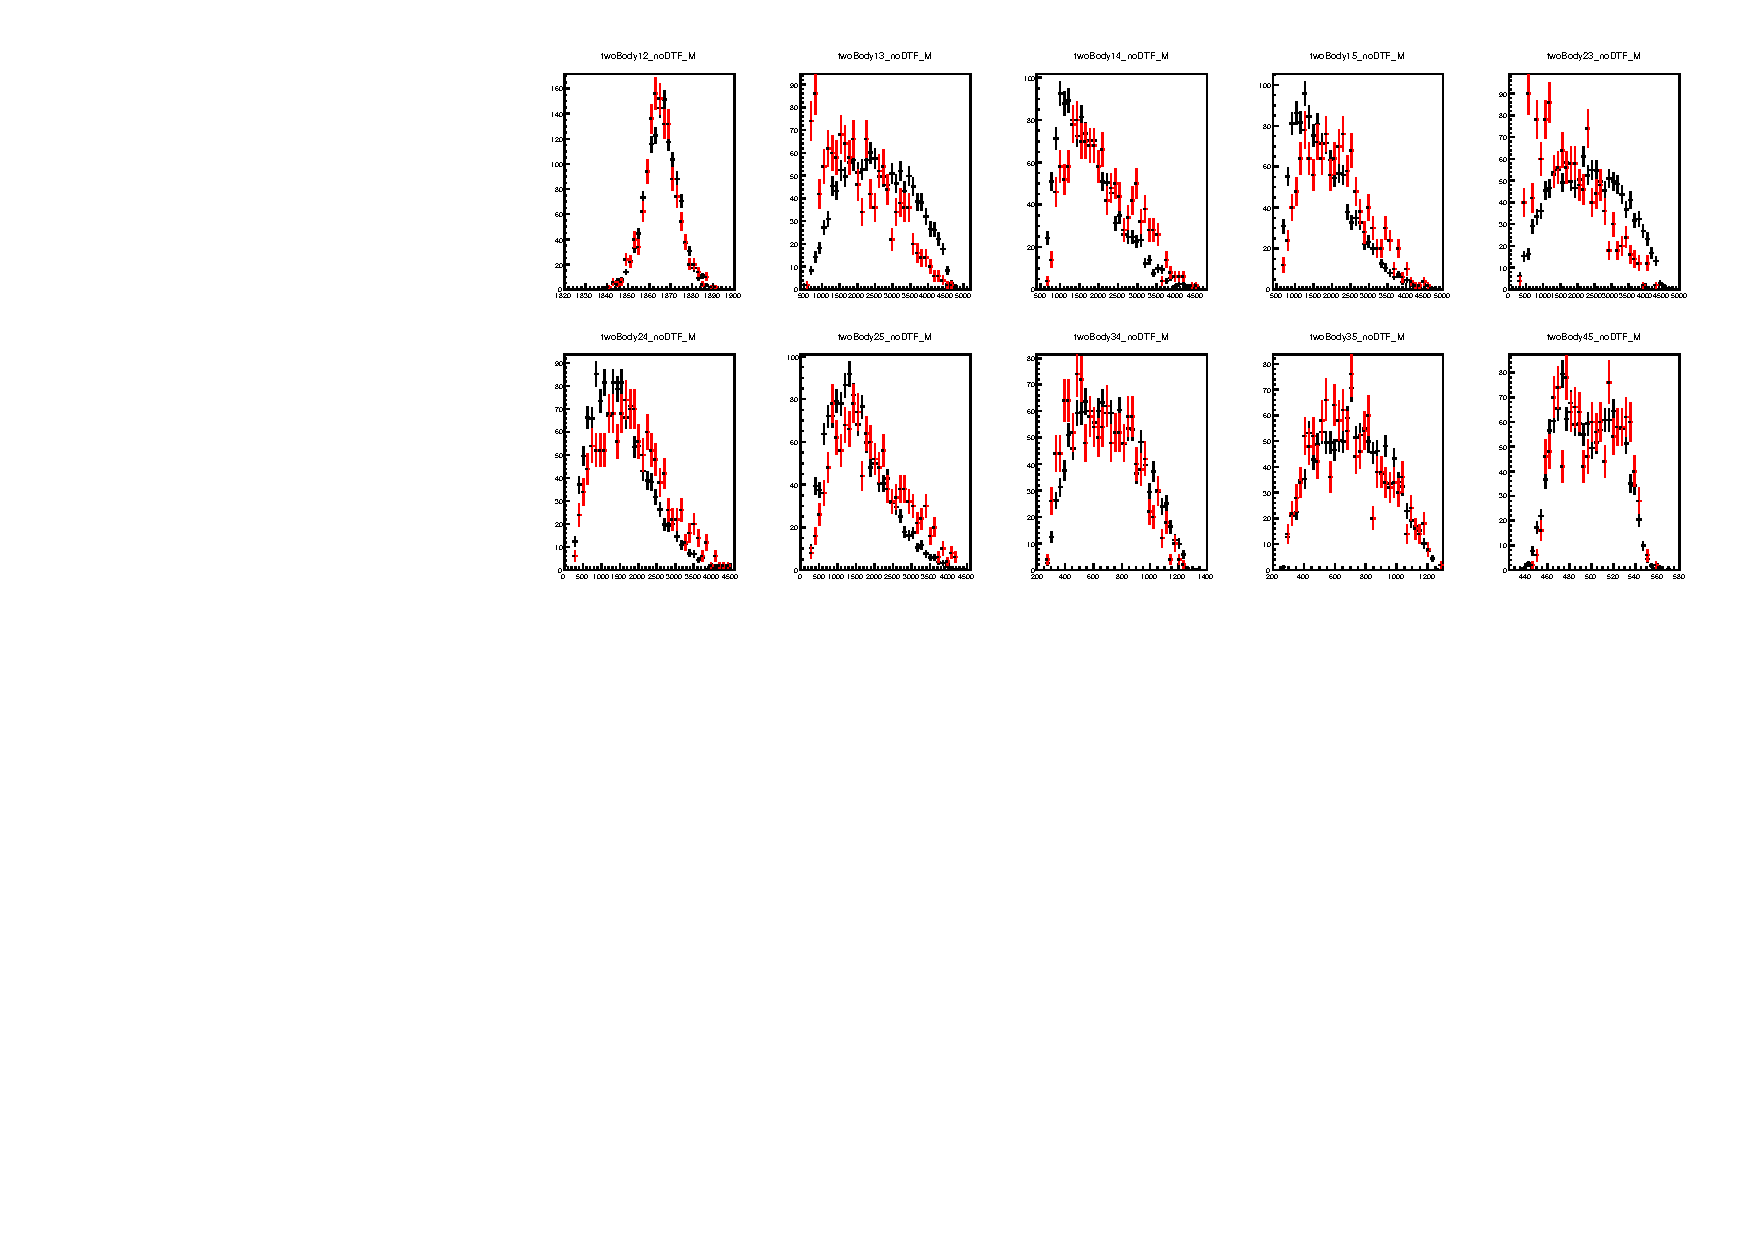
\includegraphics[width=\linewidth]{figures/massProjections/massProjectionsDD_2body_nodtf.pdf}}
\caption{Invariant mass projections of all of the possible two body combinations of the five final state particles. Comparing \decay{\Dz}{\Km\pip} (black) and \decay{\Dz}{\Kp\pim} (red) using Run 1 and Run 2 data in the high B mass region ($>$ 5400 \mevcc) with the full selection, except for the \Kstar mass window is widened to 500 \mev and there is no \KS helicity angle requirement. Also, the tightened BDT cut in the ADS mode is not applied. The invariant masses are constructed from the various particle momenta without DTF constraints applied.}
\label{projections2bodynodtf}
\end{figure}

\begin{figure}
\subfloat[LL candidates]{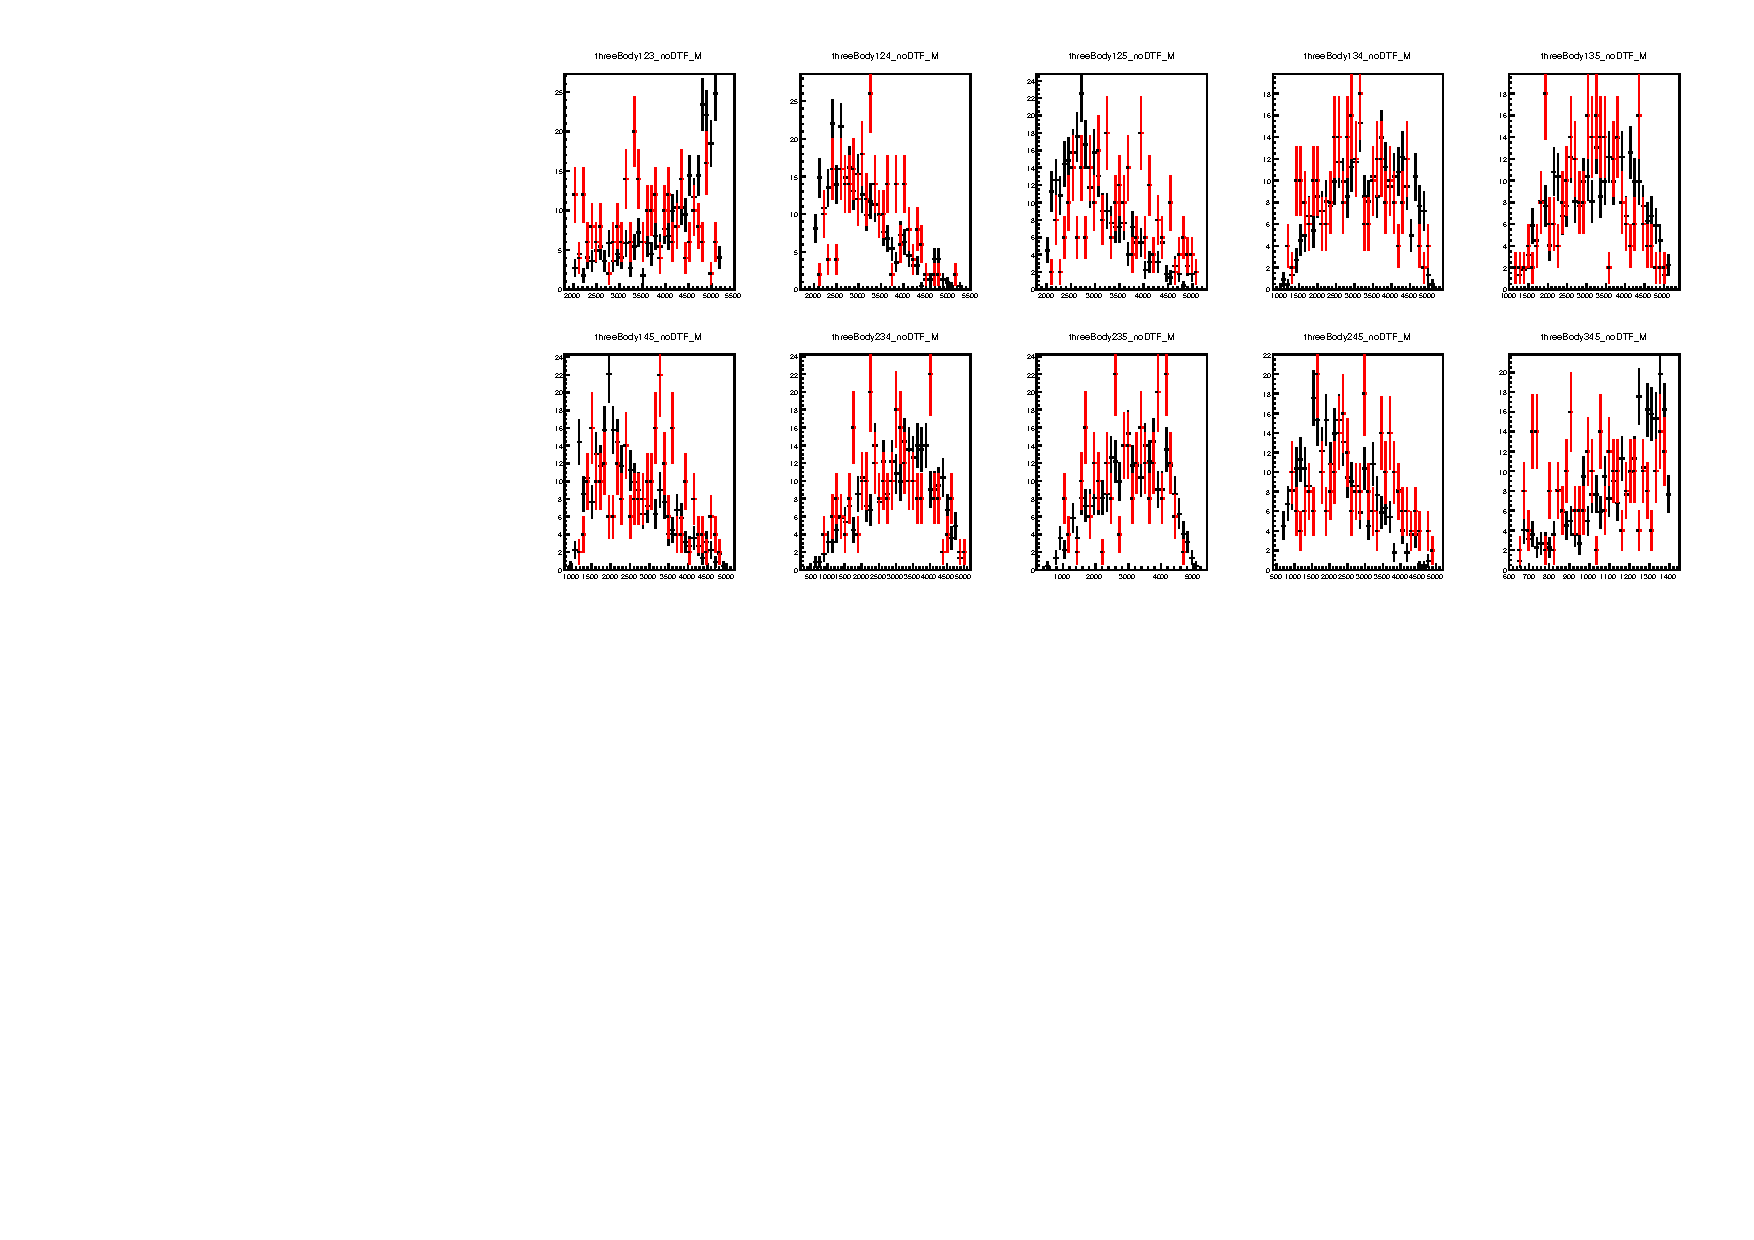
\includegraphics[width=\linewidth]{figures/massProjections/massProjectionsLL_3body_nodtf.pdf}}
\hfill
\subfloat[DD candidates]{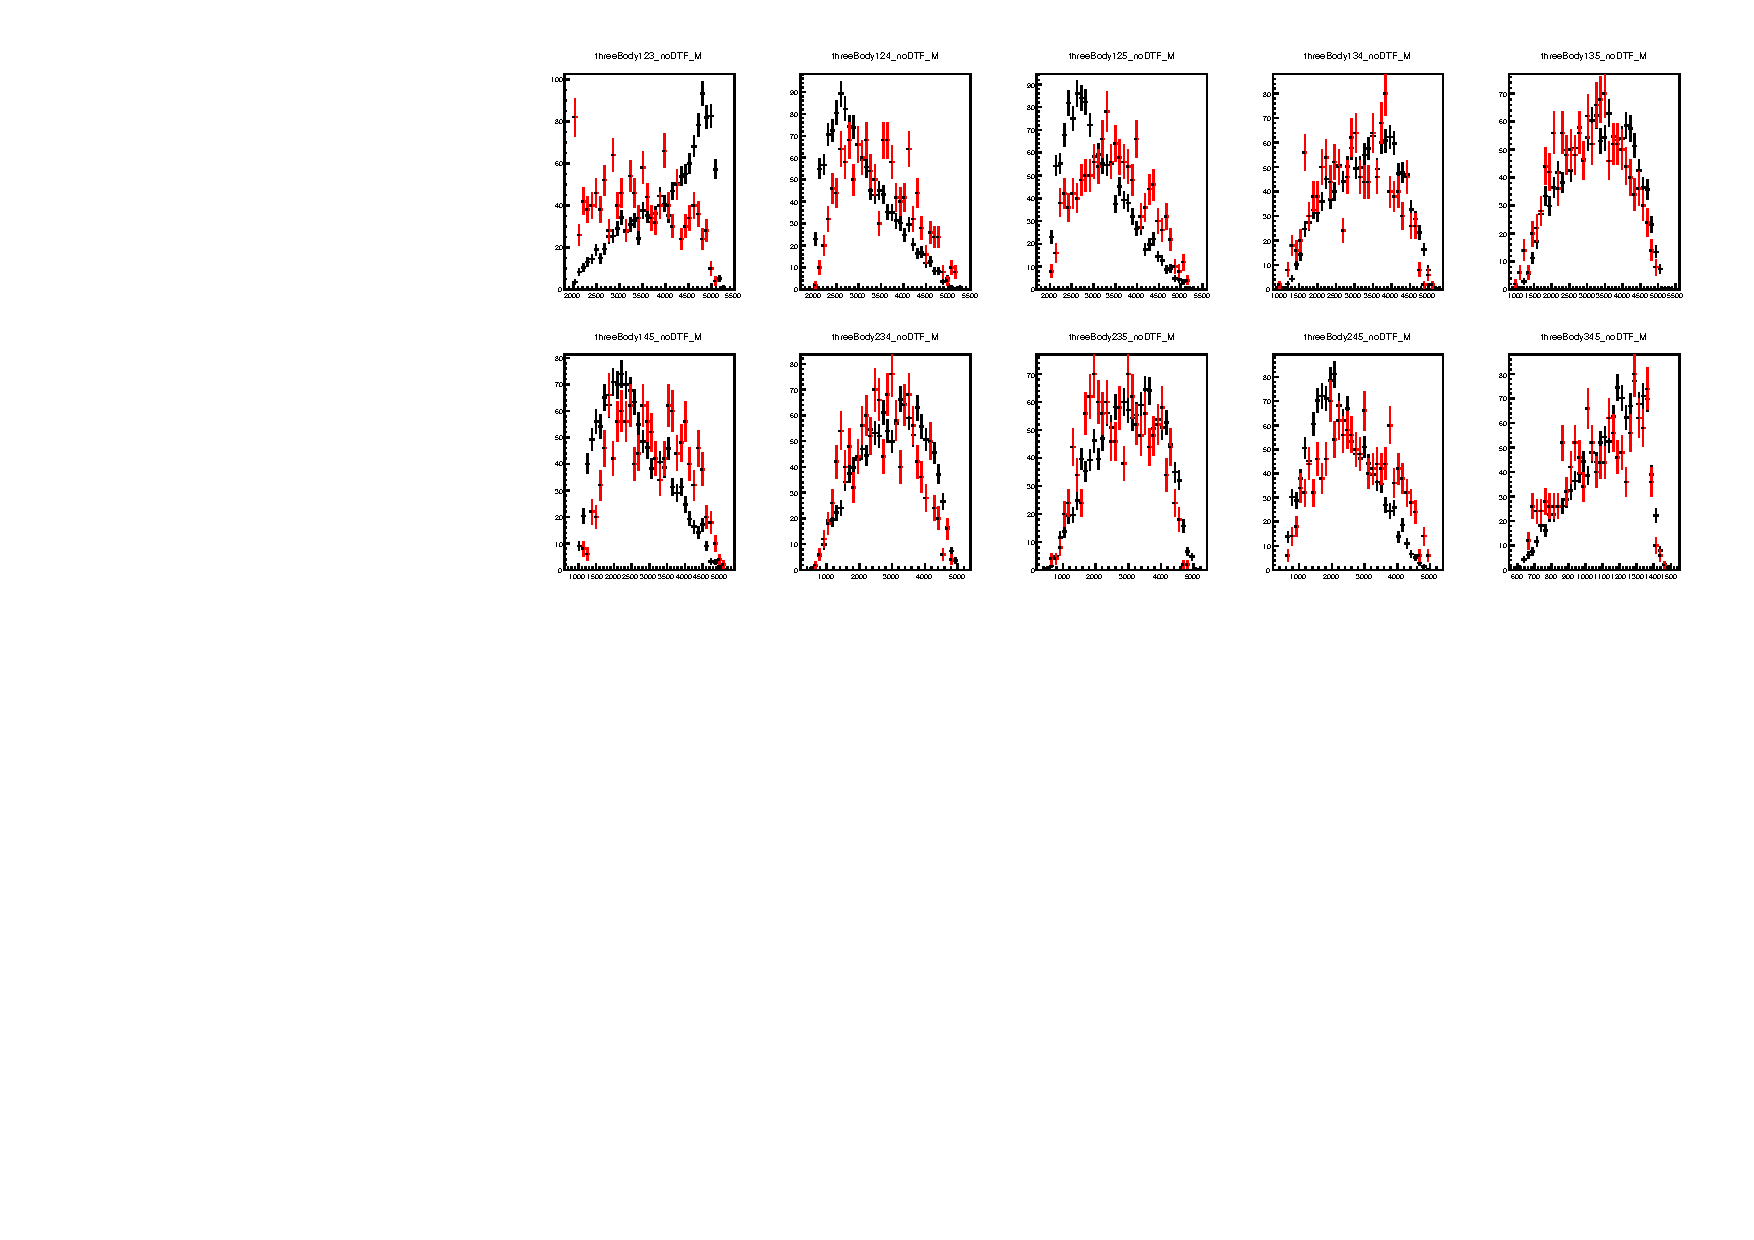
\includegraphics[width=\linewidth]{figures/massProjections/massProjectionsDD_3body_nodtf.pdf}}
\caption{Invariant mass projections of all of the possible three body combinations of the five final state particles. Comparing \decay{\Dz}{\Km\pip} (black) and \decay{\Dz}{\Kp\pim} (red) using Run 1 and Run 2 data in the high B mass region ($>$ 5400 \mevcc) with the full selection, except for the \Kstar mass window is widened to 500 \mev and there is no \KS helicity angle requirement. Also, the tightened BDT cut in the ADS mode is not applied. The invariant masses are constructed from the various particle momenta without DTF constraints applied.}
\label{projections3bodynodtf}
\end{figure}

\begin{figure}
\subfloat[2 body]{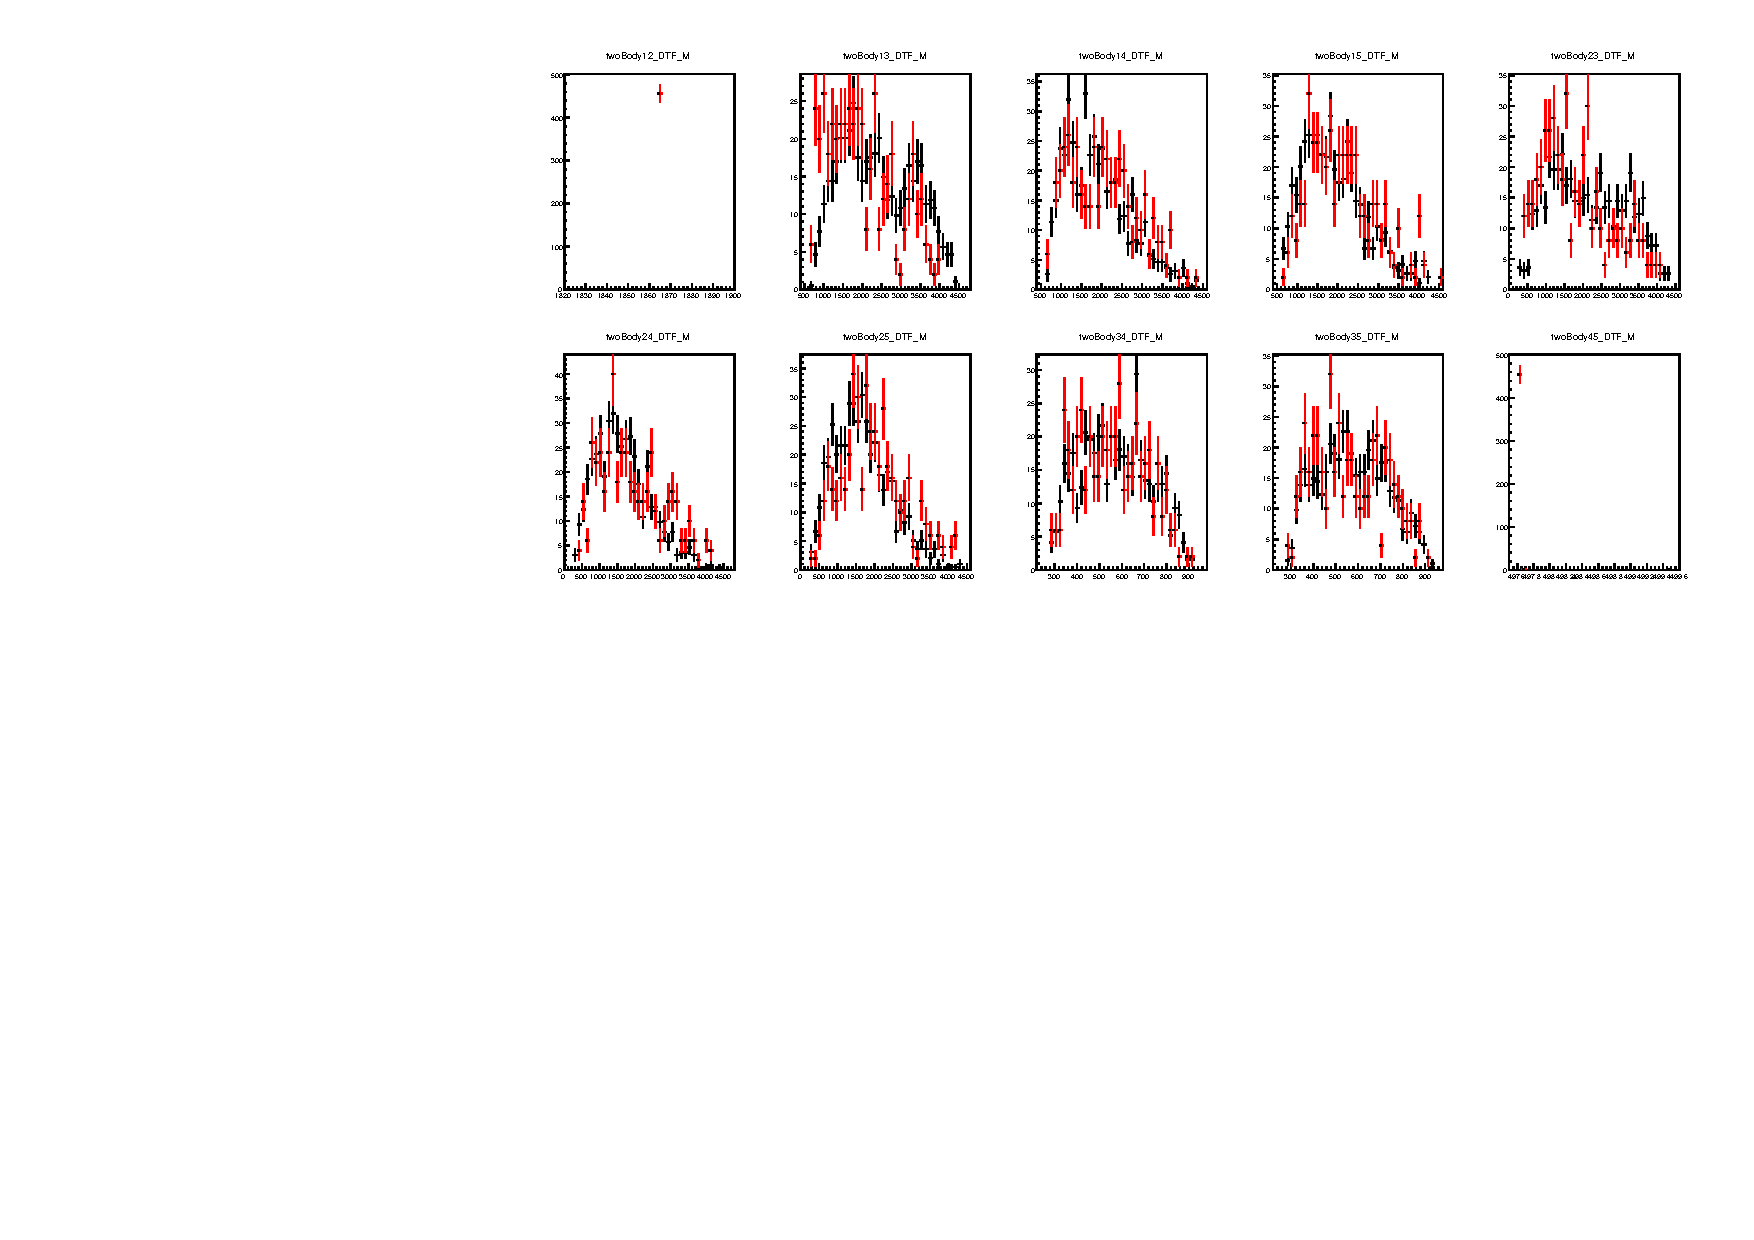
\includegraphics[width=\linewidth]{figures/massProjections/massProjectionsDD_2body_dtf_tighter.pdf}}
\hfill
\subfloat[3 body]{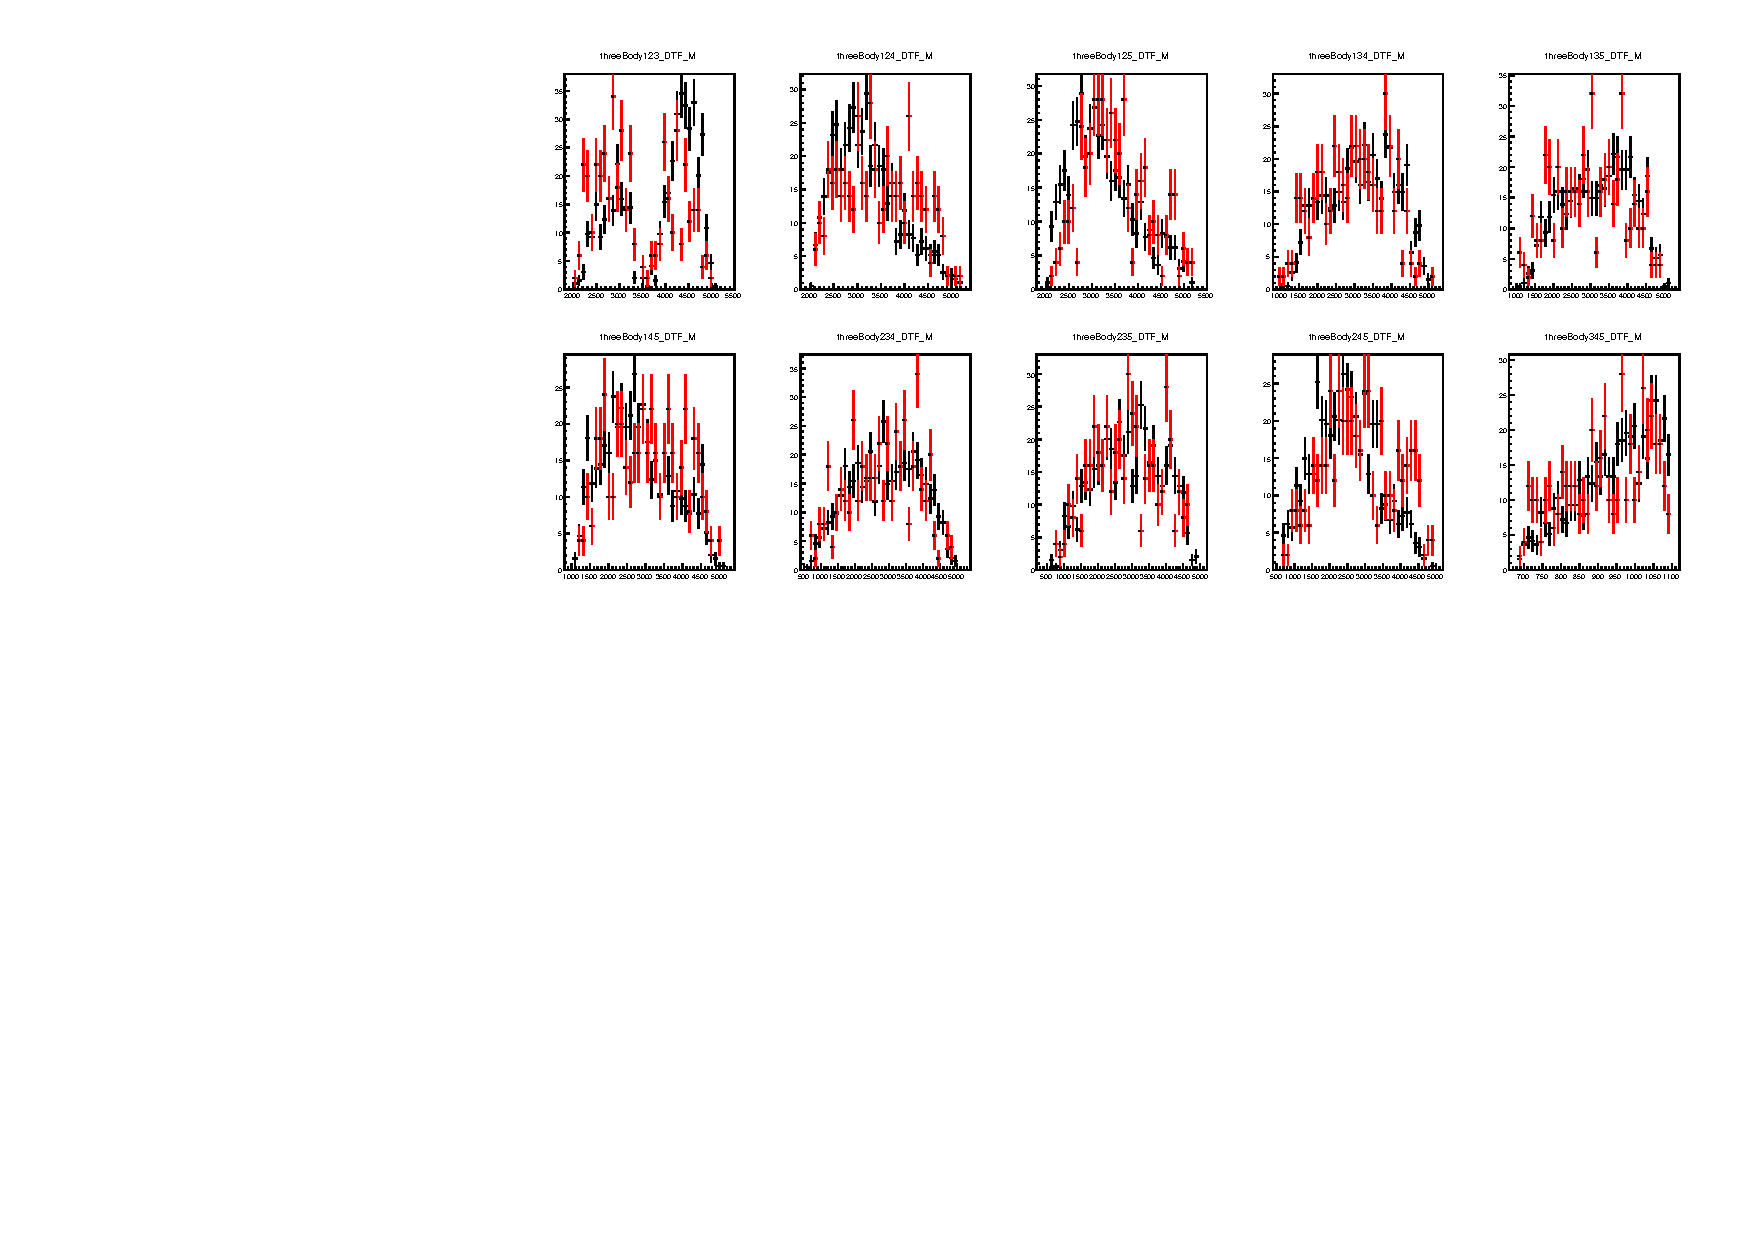
\includegraphics[width=\linewidth]{figures/massProjections/massProjectionsDD_3body_dtf_tighter.pdf}}
\caption{Invariant mass projections of all of the possible (a) two, and (b) three body combinations of the five final state particles for DD candidates only. Comparing \decay{\Dz}{\Km\pip} (black) and \decay{\Dz}{\Kp\pim} (red) using Run 1 and Run 2 data in the high B mass region ($>$ 5400 \mevcc) with the full selection, including the \KS helicity angle requirement and \Kstar mass window is 200 \mev. Also, the tightened BDT cut in the ADS mode is not applied. The invariant mass combination 12 and 45 have been constrained to be the \Dz mass and \KS mass respectively.}
\label{projectionstighter}
\end{figure}

\begin{figure}
\subfloat[looser \Kstar selection]{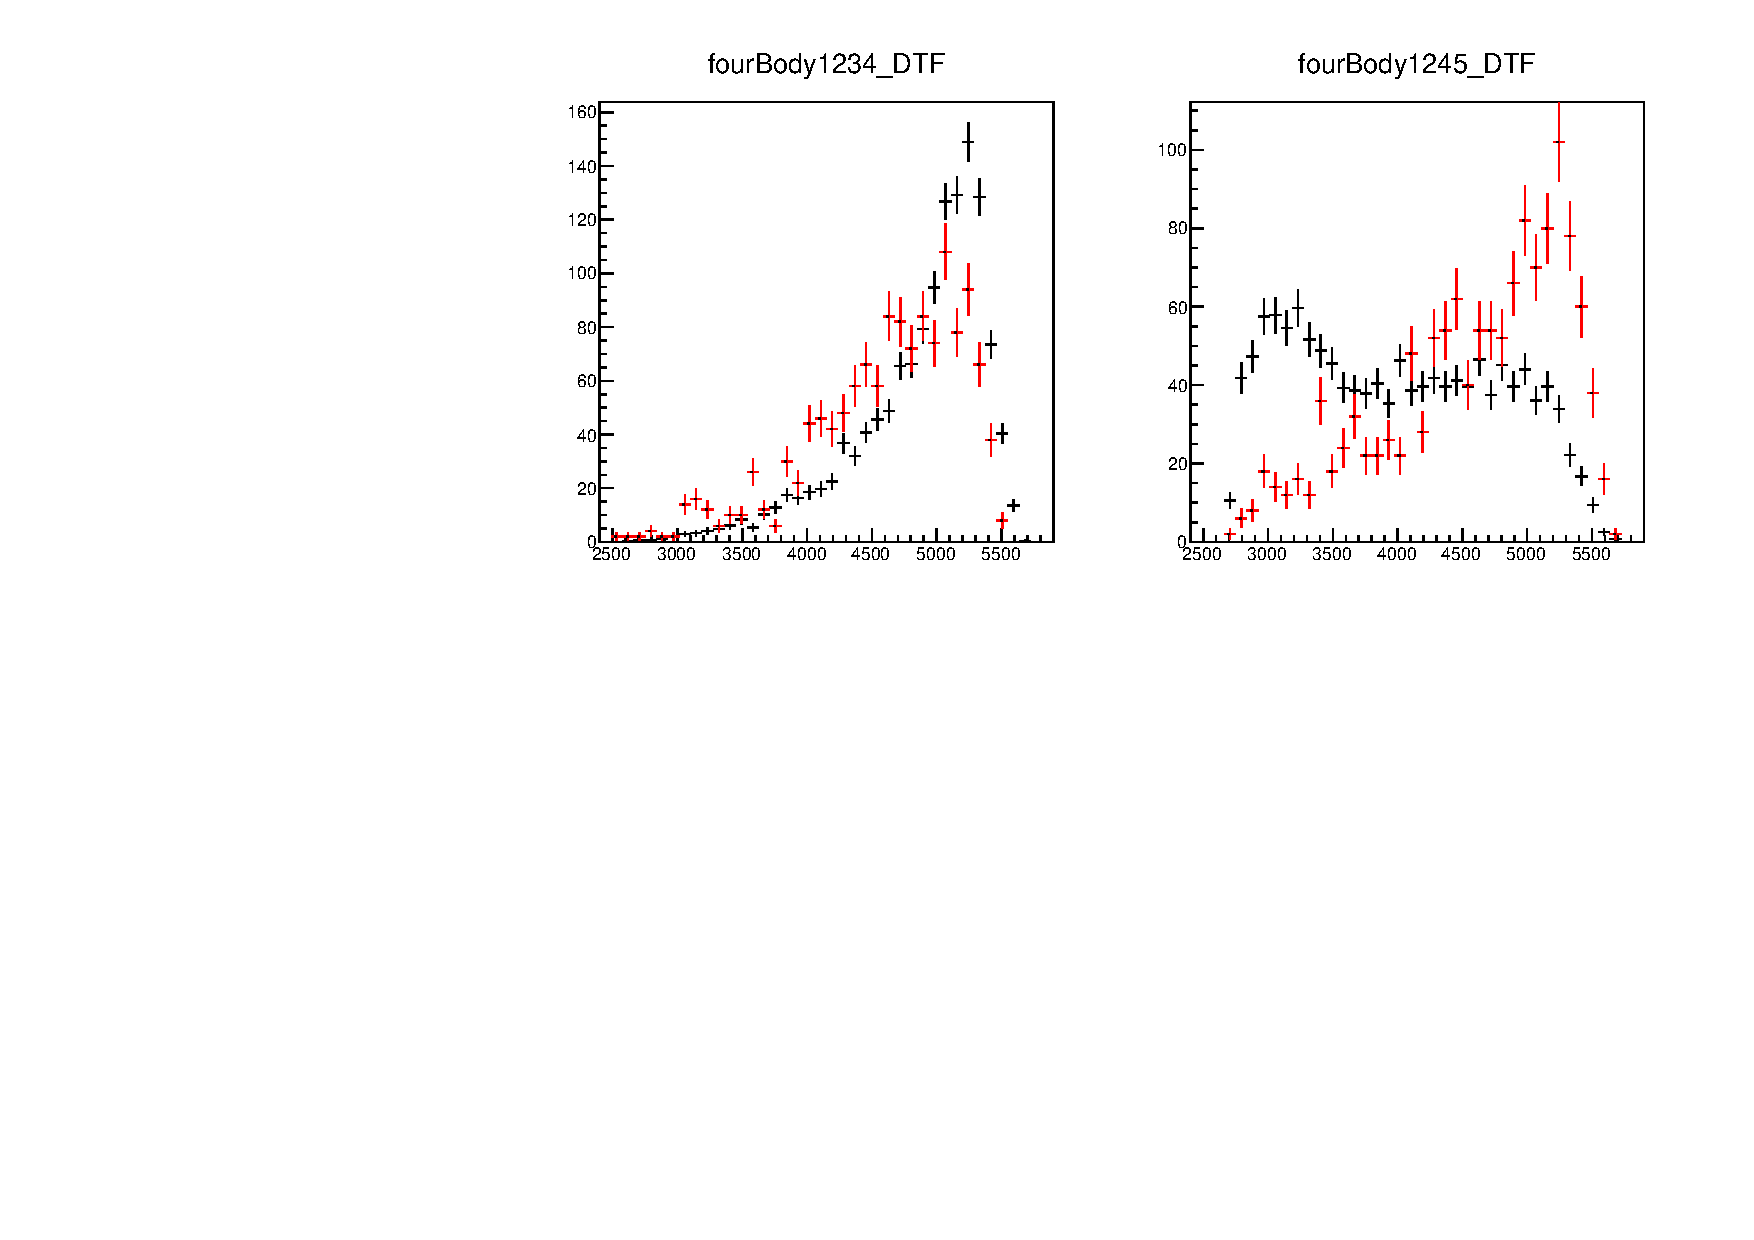
\includegraphics[width=\linewidth]{figures/massProjections/fourBodyDD_dtf.pdf}}
\hfill
\subfloat[full \Kstar selection]{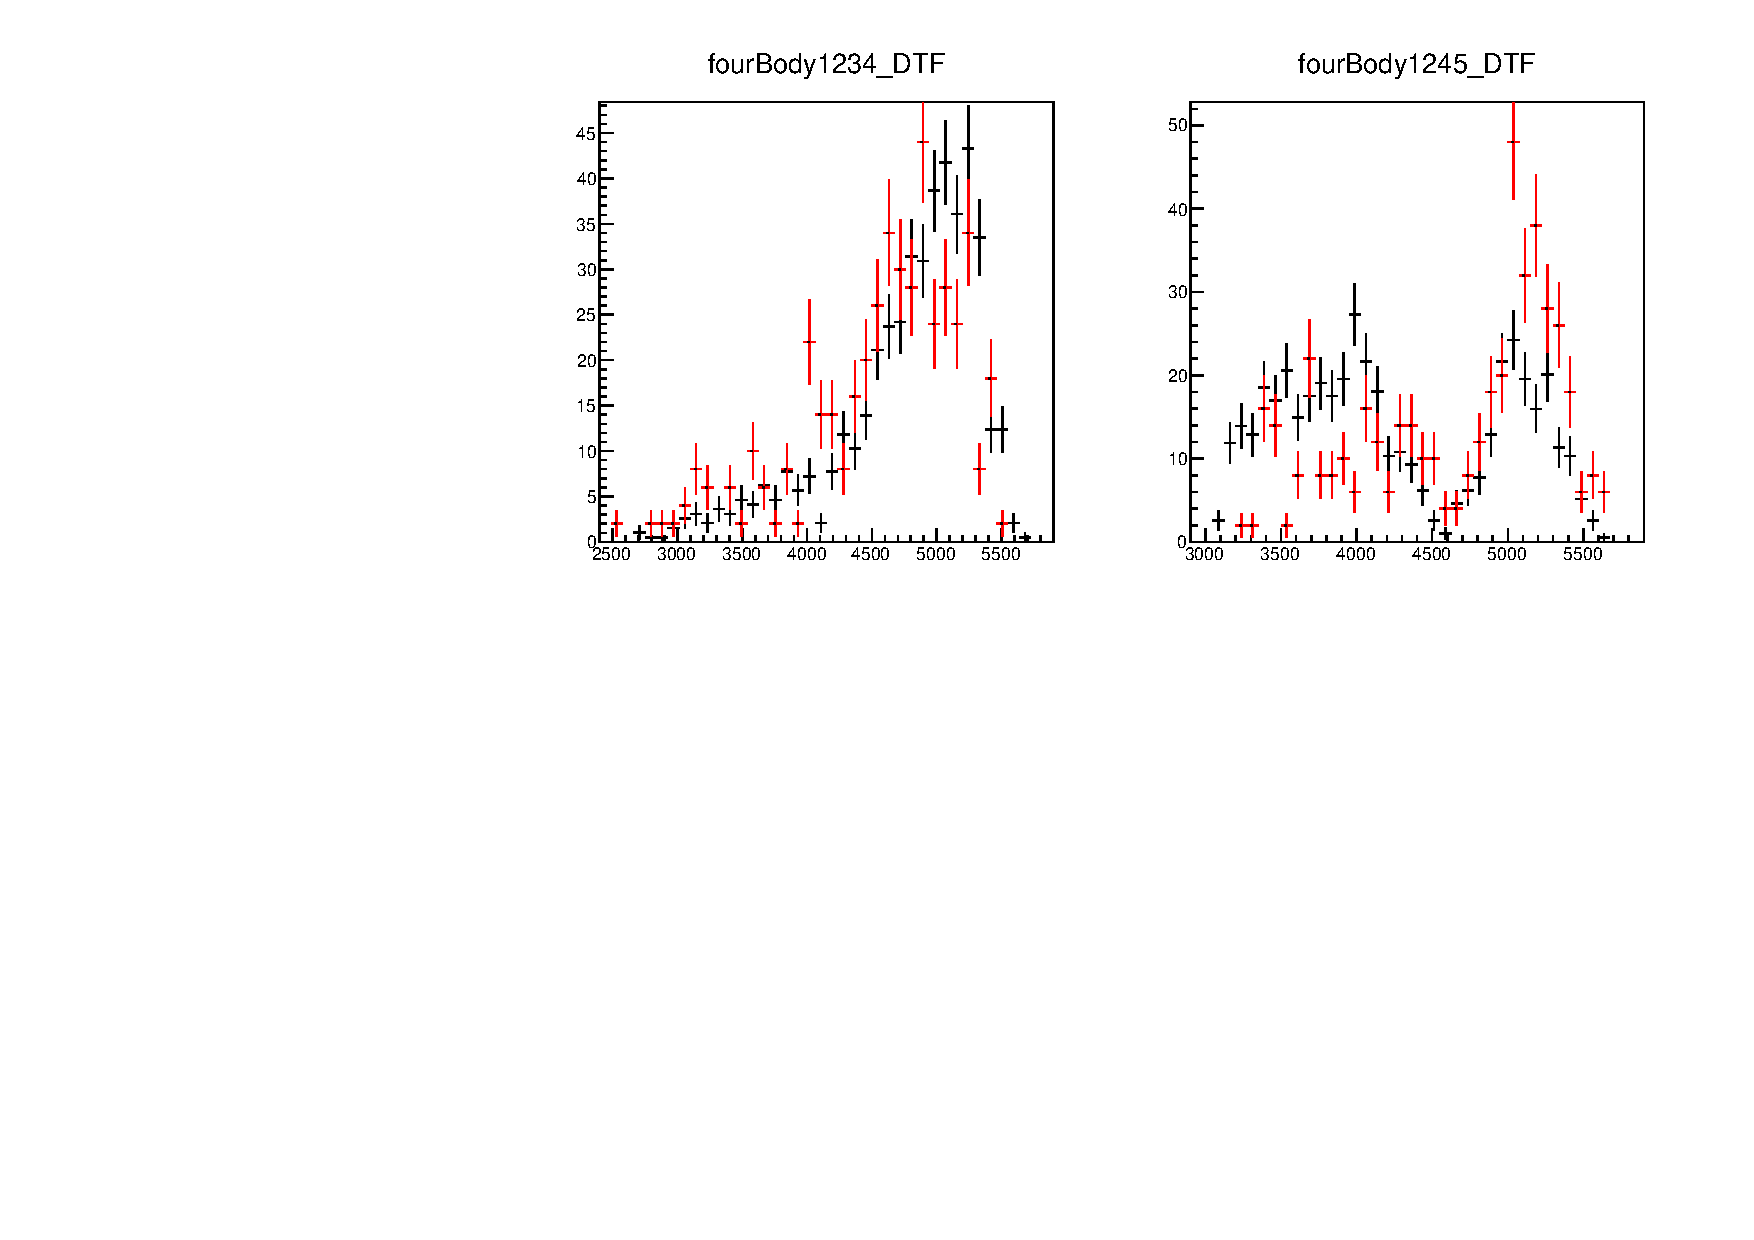
\includegraphics[width=\linewidth]{figures/massProjections/fourBodyDD_dtf_tighter.pdf}}
\caption{Invariant mass projections of two different four body combinations of the five final state particles for DD candidates only. Comparing \decay{\Dz}{\Km\pip} (black) and \decay{\Dz}{\Kp\pim} (red) using Run 1 and Run 2 data in the high B mass region ($>$ 5400 \mevcc) with the full selection, (a) the \Kstar mass window is widened to 500 \mev and there is no \KS helicity angle requirement, (b) the \KS helicity angle requirement and \Kstar mass window is 200 \mev. Also, the tightened BDT cut in the ADS mode is not applied. The invariant mass combination 12 and 45 have been constrained to be the \Dz mass and \KS mass respectively.}
\label{projection4pions}
\end{figure}

%\begin{figure}
%\subfloat[LL candidates]{\includegraphics[width=\linewidth]{twoBodyLL_Bsideband_nodtf.pdf}}
%\hfill
%\subfloat[DD candidates]{\includegraphics[width=\linewidth]{twoBodyDD_Bsideband_nodtf.pdf}}
%\caption{Invariant mass projection of all of the possible two body combinations of the five final state particles. Comparing \decay{\Dz}{\Km\pip} (black) and \decay{\Dz}{\Kp\pim} (red) using Run 1 and Run 2 data in the high B mass region ($>$ 5400 \mevcc) with the full selection, except for the \Kstar mass window is widened to 500 \mev and there is no \KS helicity angle requirement. Also, the tightened BDT cut in the ADS mode is not applied. The invariant masses are constructed from the various particle momenta without DTF constraints applied.}
%\label{compareprojections2body_nodtf}
%\end{figure}
%
%\begin{figure}
%\subfloat[LL candidates]{\includegraphics[width=\linewidth]{threeBodyLL_Bsideband_nodtf.pdf}}
%\hfill
%\subfloat[DD candidates]{\includegraphics[width=\linewidth]{threeBodyDD_Bsideband_nodtf.pdf}}
%\caption{Invariant mass projection of all of the possible three body combinations of the five final state particles. Comparing \decay{\Dz}{\Km\pip} (black) and \decay{\Dz}{\Kp\pim} (red) using Run 1 and Run 2 data in the high B mass region ($>$ 5400 \mevcc) with the full selection, except for the \Kstar mass window is widened to 500 \mev and there is no \KS helicity angle requirement. Also, the tightened BDT cut in the ADS mode is not applied. The invariant masses are constructed from the various particle momenta without DTF constraints applied.}
%\label{compareprojections3body_nodtf}
%\end{figure}
%
%\begin{figure}
%\subfloat[LL candidates]{\includegraphics[width=\linewidth]{twoBodyLL_Bsideband_dtf.pdf}}
%\hfill
%\subfloat[DD candidates]{\includegraphics[width=\linewidth]{twoBodyDD_Bsideband_dtf.pdf}}
%\caption{Invariant mass projection of all of the possible two body combinations of the five final state particles. Comparing \decay{\Dz}{\Km\pip} (black) and \decay{\Dz}{\Kp\pim} (red) using Run 1 and Run 2 data in the high B mass region ($>$ 5400 \mevcc) with the full selection, except for the \Kstar mass window is widened to 500 \mev and there is no \KS helicity angle requirement. Also, the tightened BDT cut in the ADS mode is not applied. The invariant masses are constructed from the various particle momenta with DTF constraints applied. The invariant mass combination 12 and 45 have been constrained to be the \Dz mass and \KS mass respectively.}
%\label{compareprojections2body_dtf}
%\end{figure}
%
%\begin{figure}
%\subfloat[LL candidates]{\includegraphics[width=\linewidth]{threeBodyLL_Bsideband_dtf.pdf}}
%\hfill
%\subfloat[DD candidates]{\includegraphics[width=\linewidth]{threeBodyDD_Bsideband_dtf.pdf}}
%\caption{Invariant mass projection of all of the possible three body combinations of the five final state particles. Comparing \decay{\Dz}{\Km\pip} (black) and \decay{\Dz}{\Kp\pim} (red) using Run 1 and Run 2 data in the high B mass region ($>$ 5400 \mevcc) with the full selection, except for the \Kstar mass window is widened to 500 \mev and there is no \KS helicity angle requirement. Also, the tightened BDT cut in the ADS mode is not applied. The invariant masses are constructed from the various particle momenta with DTF constraints applied.}
%\label{compareprojections3body_dtf}
%\end{figure}
%
%
%\begin{figure}
%\subfloat[LL candidates]{\includegraphics[width=0.5\linewidth]{DpurityLL_Bsideband_nodtf.pdf}}
%\hfill
%\subfloat[DD candidates]{\includegraphics[width=0.5\linewidth]{DpurityDD_Bsideband_nodtf.pdf}}
%\caption{Reconstructed mass of the \D meson in the high B mass sideband ($>$ 5400 \mev) using Run 1 and Run 2 data and applying the modified selection with no DTF variables}
%\label{Dpurity}
%\end{figure}

\newpage
\clearpage

\subsection{Further cross checks}

Table \ref{combinatoricyields} shows a comparison of the combinatoic yield from the simultaneous fit. In order to make a fair comparison the BDT selection in the ADS mode is loosened to match that in the CF, and the double misID veto is applied to both the CF and ADS modes.

\begin{table}[!h]
\centering
\begin{tabular}{c|cccc}
& Run 1 LL & Run 1 DD & Run 2 LL & Run 2 DD \\
\hline
$K\pi$ & $17 \pm 5$ & $115 \pm 13$ & $33 \pm 5$ & $296 \pm 22$ \\
$\pi K$ & $11 \pm 4$ & $26 \pm 6$ & $19 \pm 5$ & $93 \pm 11$ \\
\hline
Ratio & $0.6 \pm 0.3$ & $0.23 \pm 0.06$ & $0.6 \pm 0.2$ & $0.31 \pm 0.04$ \\
\hline
$K\pi\pi\pi$ & $2.6 \pm 2.2$ & $61 \pm 10$ & $19 \pm 6$ & $218 \pm 19$ \\
$\pi K\pi\pi$ & $3.3 \pm 2.4$ & $18 \pm 5$ & $14 \pm 5$ & $78 \pm 10$ \\
\hline
Ratio & $1.2 \pm 1.7$ & $0.30 \pm 0.10$ & $0.7 \pm 0.4$ & $0.36 \pm 0.06$ \\
\hline
\end{tabular}
\caption{Comparison of combinatoric yield from simultaneous fit}
\label{combinatoricyields}
\end{table}

\subsubsection{\KS backgrounds}

As the discrepany is found for DD candidates and not for LL, we can check for \KS backgrounds in the CF mode. Figure \ref{APplots} shows the AP plots for the combinatoric background in the CF and ADS modes, which would reveal any contamination from \Lz, see Section \ref{sec:backgrounds:contamination}. These plots show that the combinatoric background in both the CF and ADS modes is made of true \KS mesons and there is no evidence of \Lz contamination. As a further test for \Lz baryons in the combinatoric background the simultaneous fit is run with a PID cut of PIDp $>$ 0 applied to the \KS daughter pions for all the D modes. Table \ref{combyieldspidp} shows the resulting combinatoric yields extracted from the simultaneous fit. It can be seen that the discrepancy of yields between the suppressed and favoured mode for 2 and 4 body is not improved with the PIDp cut. 

In conclusion, there is no evidence for \Lz contamination and this is definitely not the cause of the inconsistency between the CF and ADS yields.

\begin{figure}
\includegraphics[width=0.5\linewidth]{figures/massProjections/applot_KPicombinatoric_LL.pdf}
\hfill
\includegraphics[width=0.5\linewidth]{figures/massProjections/applot_KPicombinatoric_DD.pdf}
\hfill
\includegraphics[width=0.5\linewidth]{figures/massProjections/applot_KPi2combinatoric_LL.pdf}
\hfill
\includegraphics[width=0.5\linewidth]{figures/massProjections/applot_KPi2combinatoric_DD.pdf}
\caption{AP plots for the combinatoric background}
\label{APplots}
\end{figure}

\begin{table}[!h]
\centering
\begin{tabular}{c|cccc}
& Run 1 LL & Run 1 DD & Run 2 LL & Run 2 DD \\
\hline
$K\pi$ & $9.9 \pm 4.1$ & $32 \pm 7$ & $24 \pm 6$ & $212 \pm 19$ \\
$\pi K$ & $7.8 \pm 3.4$ & $11 \pm 4$ & $17 \pm 5$ & $55 \pm 8$ \\
\hline
Ratio & $0.8 \pm 0.5$ & $0.34 \pm 0.15$ & $0.7 \pm 0.3$ & $0.26 \pm 0.04$ \\
\hline
$K\pi\pi\pi$ & $1.2 \pm 2.0$ & $32 \pm 7$ & $11 \pm 4$ & $143 \pm 16$ \\
$\pi K\pi\pi$ & $1.0 \pm 1.4$ & $6.0 \pm 1.8$ & $10 \pm 4$ & $49 \pm 8$ \\
\hline
Ratio & $0.8 \pm 1.8$ & $0.19 \pm 0.07$ & $0.9 \pm 0.5$ & $0.34 \pm 0.07$ \\
\hline
\end{tabular}
\caption{Combinatoric yields with a PIDp $>$ 0 cut applied to the \KS daughter pions}
\label{combyieldspidp}
\end{table}

Another possibility is some detector effect. If there is a real long pion track where the \velo doesn't match so it looks like a down track, and then it could combined with another down track to make a fake \KS. Therefore, we also test against fake \KS. Table \ref{fakeks} shows the results of the combinatoric yields when the fit is run applying a Ks FD significance cut $>$ 5 to DD candidates as well as LL. 

\begin{table}[!h]
\centering
\begin{tabular}{c|cccc}
& Run 1 LL & Run 1 DD & Run 2 LL & Run 2 DD \\
\hline
$K\pi$ & $17 \pm 5$ & $110 \pm 13$ & $33 \pm 8$ & $287 \pm 22$ \\
$\pi K$ & $12 \pm 4$ & $25 \pm 6$ & $19 \pm 5$ & $89 \pm 10$ \\
\hline
Ratio & $0.7 \pm 0.3$ & $0.23 \pm 0.06$ & $0.6 \pm 0.2$ & $0.31 \pm 0.04$ \\
\hline
$K\pi\pi\pi$ & $2.6 \pm 2.2$ & $57 \pm 9$ & $19 \pm 6$ & $206 \pm 18$ \\
$\pi K\pi\pi$ & $3.4 \pm 2.5$ & $18 \pm 5$ & $14 \pm 5$ & $78 \pm 10$ \\
\hline
Ratio & $1.3 \pm 1.5$ & $0.32 \pm 0.10$ & $0.7 \pm 0.4$ & $0.38 \pm 0.06$ \\
\hline
\end{tabular}
\caption{Combinatoric yields with a Ks FD significance $>$ 5 cut applied to DD as well as LL}
\label{fakeks}
\end{table}

\subsubsection{BDT training bias}

The BDT applied to the data is trained on signal MC as well as high B mass background ($>$ 5600 \mev) in the CF mode. As the BDT used background training data from the CF mode only this could be biasing the BDT selection resulting in a different performance between CF and ADS modes in data. (It might be thought that the training on CF background would bias the BDT to improve the removal combinatoric in the CF mode, which is the oppostite effect to that observed. Also, the discrepancy occurs at every level of the selection, not just the BDT. But we test nonetheless).

In order to check for this bias a new BDT is trained using high B mass ADS data as a training background. This new BDT is then applied to the data and the final selected cadidates are used in the simultaneous fit. Table \ref{adsbdt} shows the combinatoric yields obtained from the fit. The discrepancy of yields between the ADS and CF mode is not improved by training the BDT on the ADS background. Therefore, we can conclude that the BDT is not a cause the inconsistency.

\begin{table}[!h]
\centering
\begin{tabular}{c|cccc}
& Run 1 LL & Run 1 DD & Run 2 LL & Run 2 DD \\
\hline
$K\pi$ & $17 \pm 5$ & $167 \pm 16$ & $43 \pm 9$ & $445 \pm 26$ \\
$\pi K$ & $14 \pm 4$ & $44 \pm 7$ & $20 \pm 5$ & $120 \pm 12$ \\
\hline
Ratio & $0.8 \pm 0.3$ & $0.26 \pm 0.05$ & $0.5 \pm 0.2$ & $0.27 \pm 0.03$ \\
\hline
\end{tabular}
\caption{Combinatoric yields using BDT trained on ADS background}
\label{adsbdt}
\end{table}

\subsubsection{Understanding of CF signal}

Although the difference in combinatoric yield between the CF and ADS modes is currently unknown, this should not impact the physics results from the analysis. The only way this could impact the CP observables if the difference in combinatoric yield is an indication that we do not correctly understand our signal. In order to make sure that the signal events are what is expected we compare eefficiency in data and MC for various BDT cuts. If these are consistent this indicates that our signal in data matches what we expect from MC. Tables \ref{BDTefficiencyrun1} and \ref{BDTefficiencyrun2} show the results obtained, which confirm consistency between our data in signal and MC. This check is also done for PID efficiency are the results are found to be consistent between data and MC, the results are shown in Table \ref{PIDefficiencyrun1}.

Therefore, we can conclude that the signal is well understood and whatever the cause of the combinatoric discrepancy the physics observables are not affected.

\begin{table}[!h]
\centering
\begin{tabular}{c|ccccc}
BDT cut & 0 & 0.2 & 0.4 & 0.6 & 0.8 \\
\hline
Yield & $549 \pm 26$ & $545 \pm 26$ & $532 \pm 25$ & $513 \pm 25$ & $473 \pm 23$ \\
Efficiency from data & 1 & $0.99 \pm 0.07$ & $0.97 \pm 0.06$ & $0.93 \pm 0.06$ & $0.86 \pm 0.06$ \\
Number of MC events & 6049 & 5986 & 5871 & 5731 & 5414 \\
Efficiency from MC & 1 & $0.990 \pm 0.018$ & $0.971 \pm 0.018$ & $0.947 \pm 0.017$ & $0.895 \pm 0.017$ \\
\end{tabular}
\caption{Comparison of BDT efficiency from data and MC for Run 1}
\label{BDTefficiencyrun1}
\end{table}


\begin{table}[!h]
\centering
\begin{tabular}{c|ccccc}
BDT cut & 0 & 0.2 & 0.4 & 0.6 & 0.8 \\
\hline
Yield & $976 \pm 36$ & $962 \pm 35$ & $942 \pm 34$ & $918 \pm 33$ & $877 \pm 32$ \\
Efficiency from data & 1 & $0.99 \pm 0.05$ & $0.97 \pm 0.05$ & $0.94 \pm 0.05$ & $0.90 \pm 0.05$ \\
Number of MC events & 13614 & 13497 & 13286 & 12995 & 12383 \\
Efficiency from MC & 1 & $0.991 \pm 0.012$ & $0.976 \pm 0.012$ & $0.955 \pm 0.012$ & $0.910 \pm 0.011$ \\
\end{tabular}
\caption{Comparison of BDT efficiency from data and MC for Run 2}
\label{BDTefficiencyrun2}
\end{table}

\begin{table}[!h]
\centering
{\footnotesize
\begin{tabular}{c|ccc|ccc}
& \multicolumn{3}{c}{Bachelor cut DLLK $<$} & \multicolumn{3}{c}{D daughter cut DLLK $>/<-$ for \kaon/\pion} \\
& \multicolumn{3}{c}{(with D daughter $>$ 2 for kaons,$<$ -2 for pions)} & \multicolumn{3}{c}{(with Bachelor DLLK $<$ 4)} \\
PID selection & 4 & 2 & 0 & 4 & 2 & 0 \\
\hline
Yield & $505 \pm 24$ & $494 \pm 24$ & $459 \pm 23$ & $581 \pm 26$ & $505 \pm 24$ & $450 \pm 23$ \\
Efficiency from data & 1 & $0.98 \pm 0.07$ & $0.91 \pm 0.06$ & 1 & $0.87 \pm 0.06$ & $0.77 \pm 0.05$ \\
PID efficiency & $0.747 \pm 0.002$ & $0.727 \pm 0.002$ & $0.702 \pm 0.002$ & $0.813 \pm 0.002$ & $0.747 \pm 0.002$ & $0.673 \pm 0.002$ \\
Normalised & 1 & $0.973 \pm 0.004$ & $0.940 \pm 0.004$ & 1 & $0.919 \pm 0.003$ & $0.828 \pm 0.003$ \\
\end{tabular}}
\caption{Comparison of PID efficiency in $K\pi$ DD candidates from data and MC for Run 1}
\label{PIDefficiencyrun1}
\end{table}

\clearpage
